%Options > Configure Texmaker > Editor > Spelling Dictionary, per corrector en català

\documentclass[11pt, a4paper]{report}
\usepackage[a4paper,left=30mm,right=20mm,top=25mm,bottom=25mm]{geometry}
\sloppy %per forçar el canvi de línia si la paraula supera el marge dret
\usepackage[utf8]{inputenc}



% Per utilitzar la font Helvetica (Arial)
\renewcommand{\familydefault}{\sfdefault}
\usepackage[scaled=1]{helvet}
%\usepackage[helvet]{sfmath}
%\everymath={\sf}
%Equacions amb una font sans_serif, \mathrm{equació aquí, són les letres les que queden inclinades}
%\usepackage{arev} % sans-serif math font
%\usepackage{helvet} % sans-serif text font


% Per comptar imatges enlloc de mostrar 1.1, 1.2...
\usepackage{chngcntr}
\counterwithout{figure}{chapter}
\counterwithout{table}{chapter}
\counterwithout{equation}{chapter}

\usepackage{graphicx}
\graphicspath{{images/}} %directori amb les imatges que volem insertar
\usepackage{float} %per forçar imatges amb H
\usepackage[normalem]{ulem} %negreta múltiples línies
%\usepackage{soul}

\usepackage{caption}
\captionsetup[figure]{labelfont={},name={Figura},labelsep=period}
\captionsetup[table]{labelfont={},name={Taula},labelsep=period}


\usepackage{subcaption}
\usepackage{amsmath} %per fòrmules matemàtiques
\usepackage[table]{xcolor} %per colors a les taules
%\usepackage{circuitikz} %per circuits electrònics
\usepackage{siunitx} %per les labels dels components
\usepackage[american,cuteinductors,smartlabels]{circuitikz} %american/european
\usepackage{tikz} %quadrícula
\usepackage[a4paper, left=30mm, right=20mm, top=25mm, bottom=25mm]{geometry} %geometria de la pàgina, 25 però per ajustar bé
\setlength{\headsep}{20pt}
\setlength{\footskip}{25pt}
%\usepackage[a4paper, width=150mm, top=25mm, bottom=25mm]{geometry} %geometria de la pàgina
\usepackage{lipsum} %per generar dummy text
\usepackage{xpatch} %per la distància entre títol i top

%Capçaleres i peus de pàgina
\usepackage{fancyhdr}
%\pagestyle{fancy} %fancy, plain
\fancypagestyle{plain}{
  \fancyhf{}% Clear header/footer
  \fancyhead[L]{\footnotesize{Plaques solars fotovoltaiques sensoritzades per habitatge unifamiliar}}
  \fancyhead[R]{\footnotesize{Memòria}}
  \fancyfoot[R]{\footnotesize{\thepage}}
}
\pagestyle{plain}% Set page style to plain.

%\fancyhead{}
%\fancyhead[LO,LE]{PROJECTES}
%\fancyfoot{}
%\fancyfoot[LE,RO]{\thepage} %número de la pàgina, a la dreta
%\fancyfoot[LO, CE]{Capítol \thechapter} %nom del capítol, a l'esquerra
%\fancyfoot[CO, CE]{\href{https://github.com/LFanals}{Llorenç Fanals Batllori}} %nom de l'autor, al centre
% \renewcommand{\headrulewidth}{0.4pt}
%\renewcommand{\footrulewidth}{0.4pt}

%Per tenir el nombre de pàgina a l'inici d'un capítol
%\fancypagestyle{plain}{
%\fancyhf{}
%\renewcommand\headrulewidth{0pt}
%\fancyfoot[R]{\thepage}
%}

%Per configurar el color dels links i referències
\usepackage{color}
\usepackage{hyperref}
\hypersetup{
    colorlinks=true, %true si es volen links de colors
    linkcolor=black,  %colors de les referències internes, blue
    filecolor=magenta,      %magenta
    urlcolor=[rgb]{0,0,0}, %Color dels links d'Internet, sobre 255=2^8-1=2^0+...+2^7, {0,0.5,1}
}

%Bibliografia
\usepackage[backend=bibtex]{biblatex}
\addbibresource{bibliography.bib}

%Canviem el nom que hi ha per defecte als índex i altres, per passar-ho al català
\renewcommand{\contentsname}{Índex}
\renewcommand{\listfigurename}{Índex de figures}
\renewcommand{\chaptername}{Capítol}
\renewcommand{\appendixname}{Annex}
\renewcommand{\listtablename}{Índex de taules}
% \renewcommand{\figurename}{Figura} % ho tinc amb caption
% \captionsetup[table]{name=Taula} % ho tinc amb caption

\definecolor{color_quadricula}{HTML}{0066ff} %color per la quadrícula

% Pels circuits
%\usepackage[american]{circuitikz}
\usetikzlibrary{calc}
\ctikzset{bipoles/thickness=1}
\ctikzset{bipoles/length=1.2cm}
\ctikzset{bipoles/diode/height=.375}
\ctikzset{bipoles/diode/width=.3}
\ctikzset{tripoles/thyristor/height=.8}
\ctikzset{tripoles/thyristor/width=1}
\ctikzset{bipoles/vsourceam/height/.initial=.7}
\ctikzset{bipoles/vsourceam/width/.initial=.7}
\tikzstyle{every node}=[font=\small]
\tikzstyle{every path}=[line width=0.8pt,line cap=round,line join=round]

%Per insertar codi
\usepackage{listings}
\usepackage{color}
\definecolor{dkgreen}{rgb}{0,0.6,0}
\definecolor{gray}{rgb}{0.5,0.5,0.5}
\definecolor{mauve}{rgb}{0.58,0,0.82}

\lstset{frame=none, %tb, none
  language=Python,
  aboveskip=5mm,
  belowskip=5mm,
  showstringspaces=false,
  columns=flexible,
  basicstyle={\normalsize\ttfamily}, %small
  numbers=none, %left
  numberstyle=\tiny\color{gray},
  keywordstyle=\color{blue},
  commentstyle=\color{dkgreen},
  stringstyle=\color{mauve},
  breaklines=true,
  breakatwhitespace=true,
  tabsize=3,
  literate={á}{{\'a}}1 {é}{{\'e}}1 {ó}{{\'o}}1 {í}{{\'i}}1 {ú}{{\'u}}1  {à}{\`{a}}1 {è}{\`{e}}1  {ò}{\`{o}}1  {ï}{\"\i}1  {ç}{\c{c}}1 ,  
}


%Per tenir el format de capítol correcte
\usepackage{titlesec}

\usepackage{etoolbox}
%\usepackage{hyperref}

%Per chapter
\titlespacing*{\chapter}{0pt}{-25pt}{11pt} %Espaiat del títol de capítol amb els altres elements
\titleformat{\chapter}[hang] %Per seguir escrivint darrera el número
{\normalfont\fontsize{11}{15}\bfseries}{\thechapter.}{0.4em}{\MakeUppercase} %\fontsize{Tamany}{Espai múltiples línies}

%Per secció
\titlespacing*{\section}{0pt}{11pt}{11pt} %Espaiat del títol de capítol amb els altres elements
\titleformat{\section}[hang] %Per seguir escrivint darrera el número
{\normalfont\fontsize{11}{15}}{\thesection.}{0.4em}{\bfseries} %\fontsize{Tamany}{Espai múltiples línies}

%Per subsecció
\titlespacing*{\subsection}{0pt}{11pt}{11pt} %Espaiat del títol de capítol amb els altres elements
\titleformat{\subsection}[hang] %Per seguir escrivint darrera el número
{\normalfont\fontsize{11}{15}}{\thesubsection.}{0.4em}{} %\fontsize{Tamany}{Espai múltiples línies}

%Per paràgraf
\titlespacing*{\paragraph}{0pt}{0pt}{22pt} %Espaiat del títol de capítol amb els altres elements
\titleformat{\paragraph}[hang] %Per seguir escrivint darrera el número
{\normalfont\fontsize{11}{15}}{}{}{} %\fontsize{Tamany}{Espai múltiples línies}


%Interlineat, 1.2*1.25=1.5
\linespread{1.25}

%Espaiat entre paràgrafs
%\setlength{\parskip}{22pt}
 

\makeatletter
\def\tagform@#1{\maketag@@@{(\ignorespaces{Eq.~#1}\unskip)}}
\makeatother



%Per no tenir negreta a l'index
\usepackage{etoolbox}% http://ctan.org/pkg/etoolbox
\makeatletter
\patchcmd{\l@chapter}{\bfseries}{}{}{}% \patchcmd{<cmd>}{<search>}{<replace>}{<success>}{<failure>}
\makeatother

%Per tenir punts a l'índex
\makeatletter
\renewcommand*\l@chapter{\@dottedtocline{0}{0em}{1.5em}}
\makeatother

%Per taula que adapta bé els espais
\usepackage{tabularx}
\usepackage{tabu} % http://mirrors.ibiblio.org/CTAN/macros/latex/contrib/tabu/tabu.pdf
\tabulinesep = 1mm
\usepackage[font=footnotesize]{caption} %Captions de les figures més petites

%Appendix
\usepackage[]{appendix} %toc, page

%Alinear al separador decimal amb espais
\usepackage{setspace}
\renewcommand*{\arraystretch}{1.25}

%Per fer el símbol de grau celsius amb \textcelsius{}
\usepackage{textcomp}


%%%%%%%%%%%%%%%%%%%%%%%%%%%%%%%%%%%%%%%%%%%%%%%%%%%%%%%%%%%%%%%%%%%%%%%%%%%%%%%% 
%%% ~ Arduino Language - Arduino IDE Colors ~                                  %%%
%%%                                                                            %%%
%%% Kyle Rocha-Brownell | 10/2/2017 | No Licence                               %%%
%%% -------------------------------------------------------------------------- %%%
%%%                                                                            %%%
%%% Place this file in your working directory (next to the latex file you're   %%%
%%% working on).  To add it to your project, place:                            %%%
%%%    %%%%%%%%%%%%%%%%%%%%%%%%%%%%%%%%%%%%%%%%%%%%%%%%%%%%%%%%%%%%%%%%%%%%%%%%%%%%%%%% 
%%% ~ Arduino Language - Arduino IDE Colors ~                                  %%%
%%%                                                                            %%%
%%% Kyle Rocha-Brownell | 10/2/2017 | No Licence                               %%%
%%% -------------------------------------------------------------------------- %%%
%%%                                                                            %%%
%%% Place this file in your working directory (next to the latex file you're   %%%
%%% working on).  To add it to your project, place:                            %%%
%%%    %%%%%%%%%%%%%%%%%%%%%%%%%%%%%%%%%%%%%%%%%%%%%%%%%%%%%%%%%%%%%%%%%%%%%%%%%%%%%%%% 
%%% ~ Arduino Language - Arduino IDE Colors ~                                  %%%
%%%                                                                            %%%
%%% Kyle Rocha-Brownell | 10/2/2017 | No Licence                               %%%
%%% -------------------------------------------------------------------------- %%%
%%%                                                                            %%%
%%% Place this file in your working directory (next to the latex file you're   %%%
%%% working on).  To add it to your project, place:                            %%%
%%%    \input{arduinoLanguage.tex}                                             %%%
%%% somewhere before \begin{document} in your latex file.                      %%%
%%%                                                                            %%%
%%% In your document, place your arduino code between:                         %%%
%%%   \begin{lstlisting}[language=Arduino]                                     %%%
%%% and:                                                                       %%%
%%%   \end{lstlisting}                                                         %%%
%%%                                                                            %%%
%%% Or create your own style to add non-built-in functions and variables.      %%%
%%%                                                                            %%%
 %%%%%%%%%%%%%%%%%%%%%%%%%%%%%%%%%%%%%%%%%%%%%%%%%%%%%%%%%%%%%%%%%%%%%%%%%%%%%%%% 

\usepackage{color}
\usepackage{listings}    
\usepackage{courier}

%%% Define Custom IDE Colors %%%
\definecolor{arduinoGreen}    {rgb} {0.17, 0.43, 0.01}
\definecolor{arduinoGrey}     {rgb} {0.47, 0.47, 0.33}
\definecolor{arduinoOrange}   {rgb} {0.8 , 0.4 , 0   }
\definecolor{arduinoBlue}     {rgb} {0.01, 0.61, 0.98}
\definecolor{arduinoDarkBlue} {rgb} {0.0 , 0.2 , 0.5 }

%%% Define Arduino Language %%%
\lstdefinelanguage{Arduino}{
  language=C++, % begin with default C++ settings 
%
%
  %%% Keyword Color Group 1 %%%  (called KEYWORD3 by arduino)
  keywordstyle=\color{arduinoGreen},   
  deletekeywords={  % remove all arduino keywords that might be in c++
                break, case, override, final, continue, default, do, else, for, 
                if, return, goto, switch, throw, try, while, setup, loop, export, 
                not, or, and, xor, include, define, elif, else, error, if, ifdef, 
                ifndef, pragma, warning,
                HIGH, LOW, INPUT, INPUT_PULLUP, OUTPUT, DEC, BIN, HEX, OCT, PI, 
                HALF_PI, TWO_PI, LSBFIRST, MSBFIRST, CHANGE, FALLING, RISING, 
                DEFAULT, EXTERNAL, INTERNAL, INTERNAL1V1, INTERNAL2V56, LED_BUILTIN, 
                LED_BUILTIN_RX, LED_BUILTIN_TX, DIGITAL_MESSAGE, FIRMATA_STRING, 
                ANALOG_MESSAGE, REPORT_DIGITAL, REPORT_ANALOG, SET_PIN_MODE, 
                SYSTEM_RESET, SYSEX_START, auto, int8_t, int16_t, int32_t, int64_t, 
                uint8_t, uint16_t, uint32_t, uint64_t, char16_t, char32_t, operator, 
                enum, delete, bool, boolean, byte, char, const, false, float, double, 
                null, NULL, int, long, new, private, protected, public, short, 
                signed, static, volatile, String, void, true, unsigned, word, array, 
                sizeof, dynamic_cast, typedef, const_cast, struct, static_cast, union, 
                friend, extern, class, reinterpret_cast, register, explicit, inline, 
                _Bool, complex, _Complex, _Imaginary, atomic_bool, atomic_char, 
                atomic_schar, atomic_uchar, atomic_short, atomic_ushort, atomic_int, 
                atomic_uint, atomic_long, atomic_ulong, atomic_llong, atomic_ullong, 
                virtual, PROGMEM,
                Serial, Serial1, Serial2, Serial3, SerialUSB, Keyboard, Mouse,
                abs, acos, asin, atan, atan2, ceil, constrain, cos, degrees, exp, 
                floor, log, map, max, min, radians, random, randomSeed, round, sin, 
                sq, sqrt, tan, pow, bitRead, bitWrite, bitSet, bitClear, bit, 
                highByte, lowByte, analogReference, analogRead, 
                analogReadResolution, analogWrite, analogWriteResolution, 
                attachInterrupt, detachInterrupt, digitalPinToInterrupt, delay, 
                delayMicroseconds, digitalWrite, digitalRead, interrupts, millis, 
                micros, noInterrupts, noTone, pinMode, pulseIn, pulseInLong, shiftIn, 
                shiftOut, tone, yield, Stream, begin, end, peek, read, print, 
                println, available, availableForWrite, flush, setTimeout, find, 
                findUntil, parseInt, parseFloat, readBytes, readBytesUntil, readString, 
                readStringUntil, trim, toUpperCase, toLowerCase, charAt, compareTo, 
                concat, endsWith, startsWith, equals, equalsIgnoreCase, getBytes, 
                indexOf, lastIndexOf, length, replace, setCharAt, substring, 
                toCharArray, toInt, press, release, releaseAll, accept, click, move, 
                isPressed, isAlphaNumeric, isAlpha, isAscii, isWhitespace, isControl, 
                isDigit, isGraph, isLowerCase, isPrintable, isPunct, isSpace, 
                isUpperCase, isHexadecimalDigit, 
                }, 
  morekeywords={   % add arduino structures to group 1
                break, case, override, final, continue, default, do, else, for, 
                if, return, goto, switch, throw, try, while, setup, loop, export, 
                not, or, and, xor, include, define, elif, else, error, if, ifdef, 
                ifndef, pragma, warning,
                }, 
% 
%
  %%% Keyword Color Group 2 %%%  (called LITERAL1 by arduino)
  keywordstyle=[2]\color{arduinoBlue},   
  keywords=[2]{   % add variables and dataTypes as 2nd group  
                HIGH, LOW, INPUT, INPUT_PULLUP, OUTPUT, DEC, BIN, HEX, OCT, PI, 
                HALF_PI, TWO_PI, LSBFIRST, MSBFIRST, CHANGE, FALLING, RISING, 
                DEFAULT, EXTERNAL, INTERNAL, INTERNAL1V1, INTERNAL2V56, LED_BUILTIN, 
                LED_BUILTIN_RX, LED_BUILTIN_TX, DIGITAL_MESSAGE, FIRMATA_STRING, 
                ANALOG_MESSAGE, REPORT_DIGITAL, REPORT_ANALOG, SET_PIN_MODE, 
                SYSTEM_RESET, SYSEX_START, auto, int8_t, int16_t, int32_t, int64_t, 
                uint8_t, uint16_t, uint32_t, uint64_t, char16_t, char32_t, operator, 
                enum, delete, bool, boolean, byte, char, const, false, float, double, 
                null, NULL, int, long, new, private, protected, public, short, 
                signed, static, volatile, String, void, true, unsigned, word, array, 
                sizeof, dynamic_cast, typedef, const_cast, struct, static_cast, union, 
                friend, extern, class, reinterpret_cast, register, explicit, inline, 
                _Bool, complex, _Complex, _Imaginary, atomic_bool, atomic_char, 
                atomic_schar, atomic_uchar, atomic_short, atomic_ushort, atomic_int, 
                atomic_uint, atomic_long, atomic_ulong, atomic_llong, atomic_ullong, 
                virtual, PROGMEM,
                },  
% 
%
  %%% Keyword Color Group 3 %%%  (called KEYWORD1 by arduino)
  keywordstyle=[3]\bfseries\color{arduinoOrange},
  keywords=[3]{  % add built-in functions as a 3rd group
                Serial, Serial1, Serial2, Serial3, SerialUSB, Keyboard, Mouse,
                },      
%
%
  %%% Keyword Color Group 4 %%%  (called KEYWORD2 by arduino)
  keywordstyle=[4]\color{arduinoOrange},
  keywords=[4]{  % add more built-in functions as a 4th group
                abs, acos, asin, atan, atan2, ceil, constrain, cos, degrees, exp, 
                floor, log, map, max, min, radians, random, randomSeed, round, sin, 
                sq, sqrt, tan, pow, bitRead, bitWrite, bitSet, bitClear, bit, 
                highByte, lowByte, analogReference, analogRead, 
                analogReadResolution, analogWrite, analogWriteResolution, 
                attachInterrupt, detachInterrupt, digitalPinToInterrupt, delay, 
                delayMicroseconds, digitalWrite, digitalRead, interrupts, millis, 
                micros, noInterrupts, noTone, pinMode, pulseIn, pulseInLong, shiftIn, 
                shiftOut, tone, yield, Stream, begin, end, peek, read, print, 
                println, available, availableForWrite, flush, setTimeout, find, 
                findUntil, parseInt, parseFloat, readBytes, readBytesUntil, readString, 
                readStringUntil, trim, toUpperCase, toLowerCase, charAt, compareTo, 
                concat, endsWith, startsWith, equals, equalsIgnoreCase, getBytes, 
                indexOf, lastIndexOf, length, replace, setCharAt, substring, 
                toCharArray, toInt, press, release, releaseAll, accept, click, move, 
                isPressed, isAlphaNumeric, isAlpha, isAscii, isWhitespace, isControl, 
                isDigit, isGraph, isLowerCase, isPrintable, isPunct, isSpace, 
                isUpperCase, isHexadecimalDigit, 
                },      
%
%
  %%% Set Other Colors %%%
  stringstyle=\color{arduinoDarkBlue},    
  commentstyle=\color{arduinoGrey},    
%          
%   
  %%%% Line Numbering %%%%
%   numbers=left,                    
  numbersep=5pt,                   
  numberstyle=\color{arduinoGrey},    
  %stepnumber=2,                      % show every 2 line numbers
%
%
  %%%% Code Box Style %%%%
  breaklines=true,                    % wordwrapping
  tabsize=2,         
  basicstyle=\ttfamily  
}                                             %%%
%%% somewhere before \begin{document} in your latex file.                      %%%
%%%                                                                            %%%
%%% In your document, place your arduino code between:                         %%%
%%%   \begin{lstlisting}[language=Arduino]                                     %%%
%%% and:                                                                       %%%
%%%   \end{lstlisting}                                                         %%%
%%%                                                                            %%%
%%% Or create your own style to add non-built-in functions and variables.      %%%
%%%                                                                            %%%
 %%%%%%%%%%%%%%%%%%%%%%%%%%%%%%%%%%%%%%%%%%%%%%%%%%%%%%%%%%%%%%%%%%%%%%%%%%%%%%%% 

\usepackage{color}
\usepackage{listings}    
\usepackage{courier}

%%% Define Custom IDE Colors %%%
\definecolor{arduinoGreen}    {rgb} {0.17, 0.43, 0.01}
\definecolor{arduinoGrey}     {rgb} {0.47, 0.47, 0.33}
\definecolor{arduinoOrange}   {rgb} {0.8 , 0.4 , 0   }
\definecolor{arduinoBlue}     {rgb} {0.01, 0.61, 0.98}
\definecolor{arduinoDarkBlue} {rgb} {0.0 , 0.2 , 0.5 }

%%% Define Arduino Language %%%
\lstdefinelanguage{Arduino}{
  language=C++, % begin with default C++ settings 
%
%
  %%% Keyword Color Group 1 %%%  (called KEYWORD3 by arduino)
  keywordstyle=\color{arduinoGreen},   
  deletekeywords={  % remove all arduino keywords that might be in c++
                break, case, override, final, continue, default, do, else, for, 
                if, return, goto, switch, throw, try, while, setup, loop, export, 
                not, or, and, xor, include, define, elif, else, error, if, ifdef, 
                ifndef, pragma, warning,
                HIGH, LOW, INPUT, INPUT_PULLUP, OUTPUT, DEC, BIN, HEX, OCT, PI, 
                HALF_PI, TWO_PI, LSBFIRST, MSBFIRST, CHANGE, FALLING, RISING, 
                DEFAULT, EXTERNAL, INTERNAL, INTERNAL1V1, INTERNAL2V56, LED_BUILTIN, 
                LED_BUILTIN_RX, LED_BUILTIN_TX, DIGITAL_MESSAGE, FIRMATA_STRING, 
                ANALOG_MESSAGE, REPORT_DIGITAL, REPORT_ANALOG, SET_PIN_MODE, 
                SYSTEM_RESET, SYSEX_START, auto, int8_t, int16_t, int32_t, int64_t, 
                uint8_t, uint16_t, uint32_t, uint64_t, char16_t, char32_t, operator, 
                enum, delete, bool, boolean, byte, char, const, false, float, double, 
                null, NULL, int, long, new, private, protected, public, short, 
                signed, static, volatile, String, void, true, unsigned, word, array, 
                sizeof, dynamic_cast, typedef, const_cast, struct, static_cast, union, 
                friend, extern, class, reinterpret_cast, register, explicit, inline, 
                _Bool, complex, _Complex, _Imaginary, atomic_bool, atomic_char, 
                atomic_schar, atomic_uchar, atomic_short, atomic_ushort, atomic_int, 
                atomic_uint, atomic_long, atomic_ulong, atomic_llong, atomic_ullong, 
                virtual, PROGMEM,
                Serial, Serial1, Serial2, Serial3, SerialUSB, Keyboard, Mouse,
                abs, acos, asin, atan, atan2, ceil, constrain, cos, degrees, exp, 
                floor, log, map, max, min, radians, random, randomSeed, round, sin, 
                sq, sqrt, tan, pow, bitRead, bitWrite, bitSet, bitClear, bit, 
                highByte, lowByte, analogReference, analogRead, 
                analogReadResolution, analogWrite, analogWriteResolution, 
                attachInterrupt, detachInterrupt, digitalPinToInterrupt, delay, 
                delayMicroseconds, digitalWrite, digitalRead, interrupts, millis, 
                micros, noInterrupts, noTone, pinMode, pulseIn, pulseInLong, shiftIn, 
                shiftOut, tone, yield, Stream, begin, end, peek, read, print, 
                println, available, availableForWrite, flush, setTimeout, find, 
                findUntil, parseInt, parseFloat, readBytes, readBytesUntil, readString, 
                readStringUntil, trim, toUpperCase, toLowerCase, charAt, compareTo, 
                concat, endsWith, startsWith, equals, equalsIgnoreCase, getBytes, 
                indexOf, lastIndexOf, length, replace, setCharAt, substring, 
                toCharArray, toInt, press, release, releaseAll, accept, click, move, 
                isPressed, isAlphaNumeric, isAlpha, isAscii, isWhitespace, isControl, 
                isDigit, isGraph, isLowerCase, isPrintable, isPunct, isSpace, 
                isUpperCase, isHexadecimalDigit, 
                }, 
  morekeywords={   % add arduino structures to group 1
                break, case, override, final, continue, default, do, else, for, 
                if, return, goto, switch, throw, try, while, setup, loop, export, 
                not, or, and, xor, include, define, elif, else, error, if, ifdef, 
                ifndef, pragma, warning,
                }, 
% 
%
  %%% Keyword Color Group 2 %%%  (called LITERAL1 by arduino)
  keywordstyle=[2]\color{arduinoBlue},   
  keywords=[2]{   % add variables and dataTypes as 2nd group  
                HIGH, LOW, INPUT, INPUT_PULLUP, OUTPUT, DEC, BIN, HEX, OCT, PI, 
                HALF_PI, TWO_PI, LSBFIRST, MSBFIRST, CHANGE, FALLING, RISING, 
                DEFAULT, EXTERNAL, INTERNAL, INTERNAL1V1, INTERNAL2V56, LED_BUILTIN, 
                LED_BUILTIN_RX, LED_BUILTIN_TX, DIGITAL_MESSAGE, FIRMATA_STRING, 
                ANALOG_MESSAGE, REPORT_DIGITAL, REPORT_ANALOG, SET_PIN_MODE, 
                SYSTEM_RESET, SYSEX_START, auto, int8_t, int16_t, int32_t, int64_t, 
                uint8_t, uint16_t, uint32_t, uint64_t, char16_t, char32_t, operator, 
                enum, delete, bool, boolean, byte, char, const, false, float, double, 
                null, NULL, int, long, new, private, protected, public, short, 
                signed, static, volatile, String, void, true, unsigned, word, array, 
                sizeof, dynamic_cast, typedef, const_cast, struct, static_cast, union, 
                friend, extern, class, reinterpret_cast, register, explicit, inline, 
                _Bool, complex, _Complex, _Imaginary, atomic_bool, atomic_char, 
                atomic_schar, atomic_uchar, atomic_short, atomic_ushort, atomic_int, 
                atomic_uint, atomic_long, atomic_ulong, atomic_llong, atomic_ullong, 
                virtual, PROGMEM,
                },  
% 
%
  %%% Keyword Color Group 3 %%%  (called KEYWORD1 by arduino)
  keywordstyle=[3]\bfseries\color{arduinoOrange},
  keywords=[3]{  % add built-in functions as a 3rd group
                Serial, Serial1, Serial2, Serial3, SerialUSB, Keyboard, Mouse,
                },      
%
%
  %%% Keyword Color Group 4 %%%  (called KEYWORD2 by arduino)
  keywordstyle=[4]\color{arduinoOrange},
  keywords=[4]{  % add more built-in functions as a 4th group
                abs, acos, asin, atan, atan2, ceil, constrain, cos, degrees, exp, 
                floor, log, map, max, min, radians, random, randomSeed, round, sin, 
                sq, sqrt, tan, pow, bitRead, bitWrite, bitSet, bitClear, bit, 
                highByte, lowByte, analogReference, analogRead, 
                analogReadResolution, analogWrite, analogWriteResolution, 
                attachInterrupt, detachInterrupt, digitalPinToInterrupt, delay, 
                delayMicroseconds, digitalWrite, digitalRead, interrupts, millis, 
                micros, noInterrupts, noTone, pinMode, pulseIn, pulseInLong, shiftIn, 
                shiftOut, tone, yield, Stream, begin, end, peek, read, print, 
                println, available, availableForWrite, flush, setTimeout, find, 
                findUntil, parseInt, parseFloat, readBytes, readBytesUntil, readString, 
                readStringUntil, trim, toUpperCase, toLowerCase, charAt, compareTo, 
                concat, endsWith, startsWith, equals, equalsIgnoreCase, getBytes, 
                indexOf, lastIndexOf, length, replace, setCharAt, substring, 
                toCharArray, toInt, press, release, releaseAll, accept, click, move, 
                isPressed, isAlphaNumeric, isAlpha, isAscii, isWhitespace, isControl, 
                isDigit, isGraph, isLowerCase, isPrintable, isPunct, isSpace, 
                isUpperCase, isHexadecimalDigit, 
                },      
%
%
  %%% Set Other Colors %%%
  stringstyle=\color{arduinoDarkBlue},    
  commentstyle=\color{arduinoGrey},    
%          
%   
  %%%% Line Numbering %%%%
%   numbers=left,                    
  numbersep=5pt,                   
  numberstyle=\color{arduinoGrey},    
  %stepnumber=2,                      % show every 2 line numbers
%
%
  %%%% Code Box Style %%%%
  breaklines=true,                    % wordwrapping
  tabsize=2,         
  basicstyle=\ttfamily  
}                                             %%%
%%% somewhere before \begin{document} in your latex file.                      %%%
%%%                                                                            %%%
%%% In your document, place your arduino code between:                         %%%
%%%   \begin{lstlisting}[language=Arduino]                                     %%%
%%% and:                                                                       %%%
%%%   \end{lstlisting}                                                         %%%
%%%                                                                            %%%
%%% Or create your own style to add non-built-in functions and variables.      %%%
%%%                                                                            %%%
 %%%%%%%%%%%%%%%%%%%%%%%%%%%%%%%%%%%%%%%%%%%%%%%%%%%%%%%%%%%%%%%%%%%%%%%%%%%%%%%% 

\usepackage{color}
\usepackage{listings}    
\usepackage{courier}

%%% Define Custom IDE Colors %%%
\definecolor{arduinoGreen}    {rgb} {0, 0, 0}
\definecolor{arduinoGrey}     {rgb} {0, 0, 0}
\definecolor{arduinoOrange}   {rgb} {0 , 0 , 0}
\definecolor{arduinoBlue}     {rgb} {0, 0, 0}
\definecolor{arduinoDarkBlue} {rgb} {0 , 0 , 0}

%%% Define Arduino Language %%%
\lstdefinelanguage{Arduino_negre}{
%  language=C++, % begin with default C++ settings 
%
%
  %%% Keyword Color Group 1 %%%  (called KEYWORD3 by arduino)
  keywordstyle=\color{arduinoGreen},   
  deletekeywords={  % remove all arduino keywords that might be in c++
                break, case, override, final, continue, default, do, else, for, 
                if, return, goto, switch, throw, try, while, setup, loop, export, 
                not, or, and, xor, include, define, elif, else, error, if, ifdef, 
                ifndef, pragma, warning,
                HIGH, LOW, INPUT, INPUT_PULLUP, OUTPUT, DEC, BIN, HEX, OCT, PI, 
                HALF_PI, TWO_PI, LSBFIRST, MSBFIRST, CHANGE, FALLING, RISING, 
                DEFAULT, EXTERNAL, INTERNAL, INTERNAL1V1, INTERNAL2V56, LED_BUILTIN, 
                LED_BUILTIN_RX, LED_BUILTIN_TX, DIGITAL_MESSAGE, FIRMATA_STRING, 
                ANALOG_MESSAGE, REPORT_DIGITAL, REPORT_ANALOG, SET_PIN_MODE, 
                SYSTEM_RESET, SYSEX_START, auto, int8_t, int16_t, int32_t, int64_t, 
                uint8_t, uint16_t, uint32_t, uint64_t, char16_t, char32_t, operator, 
                enum, delete, bool, boolean, byte, char, const, false, float, double, 
                null, NULL, int, long, new, private, protected, public, short, 
                signed, static, volatile, String, void, true, unsigned, word, array, 
                sizeof, dynamic_cast, typedef, const_cast, struct, static_cast, union, 
                friend, extern, class, reinterpret_cast, register, explicit, inline, 
                _Bool, complex, _Complex, _Imaginary, atomic_bool, atomic_char, 
                atomic_schar, atomic_uchar, atomic_short, atomic_ushort, atomic_int, 
                atomic_uint, atomic_long, atomic_ulong, atomic_llong, atomic_ullong, 
                virtual, PROGMEM,
                Serial, Serial1, Serial2, Serial3, SerialUSB, Keyboard, Mouse,
                abs, acos, asin, atan, atan2, ceil, constrain, cos, degrees, exp, 
                floor, log, map, max, min, radians, random, randomSeed, round, sin, 
                sq, sqrt, tan, pow, bitRead, bitWrite, bitSet, bitClear, bit, 
                highByte, lowByte, analogReference, analogRead, 
                analogReadResolution, analogWrite, analogWriteResolution, 
                attachInterrupt, detachInterrupt, digitalPinToInterrupt, delay, 
                delayMicroseconds, digitalWrite, digitalRead, interrupts, millis, 
                micros, noInterrupts, noTone, pinMode, pulseIn, pulseInLong, shiftIn, 
                shiftOut, tone, yield, Stream, begin, end, peek, read, print, 
                println, available, availableForWrite, flush, setTimeout, find, 
                findUntil, parseInt, parseFloat, readBytes, readBytesUntil, readString, 
                readStringUntil, trim, toUpperCase, toLowerCase, charAt, compareTo, 
                concat, endsWith, startsWith, equals, equalsIgnoreCase, getBytes, 
                indexOf, lastIndexOf, length, replace, setCharAt, substring, 
                toCharArray, toInt, press, release, releaseAll, accept, click, move, 
                isPressed, isAlphaNumeric, isAlpha, isAscii, isWhitespace, isControl, 
                isDigit, isGraph, isLowerCase, isPrintable, isPunct, isSpace, 
                isUpperCase, isHexadecimalDigit, 
                }, 
  morekeywords={   % add arduino structures to group 1
                break, case, override, final, continue, default, do, else, for, 
                if, return, goto, switch, throw, try, while, setup, loop, export, 
                not, or, and, xor, include, define, elif, else, error, if, ifdef, 
                ifndef, pragma, warning,
                }, 
% 
%
  %%% Keyword Color Group 2 %%%  (called LITERAL1 by arduino)
  keywordstyle=[2]\color{arduinoBlue},   
  keywords=[2]{   % add variables and dataTypes as 2nd group  
                HIGH, LOW, INPUT, INPUT_PULLUP, OUTPUT, DEC, BIN, HEX, OCT, PI, 
                HALF_PI, TWO_PI, LSBFIRST, MSBFIRST, CHANGE, FALLING, RISING, 
                DEFAULT, EXTERNAL, INTERNAL, INTERNAL1V1, INTERNAL2V56, LED_BUILTIN, 
                LED_BUILTIN_RX, LED_BUILTIN_TX, DIGITAL_MESSAGE, FIRMATA_STRING, 
                ANALOG_MESSAGE, REPORT_DIGITAL, REPORT_ANALOG, SET_PIN_MODE, 
                SYSTEM_RESET, SYSEX_START, auto, int8_t, int16_t, int32_t, int64_t, 
                uint8_t, uint16_t, uint32_t, uint64_t, char16_t, char32_t, operator, 
                enum, delete, bool, boolean, byte, char, const, false, float, double, 
                null, NULL, int, long, new, private, protected, public, short, 
                signed, static, volatile, String, void, true, unsigned, word, array, 
                sizeof, dynamic_cast, typedef, const_cast, struct, static_cast, union, 
                friend, extern, class, reinterpret_cast, register, explicit, inline, 
                _Bool, complex, _Complex, _Imaginary, atomic_bool, atomic_char, 
                atomic_schar, atomic_uchar, atomic_short, atomic_ushort, atomic_int, 
                atomic_uint, atomic_long, atomic_ulong, atomic_llong, atomic_ullong, 
                virtual, PROGMEM,
                },  
% 
%
  %%% Keyword Color Group 3 %%%  (called KEYWORD1 by arduino)
  keywordstyle=[3]\bfseries\color{arduinoOrange},
  keywords=[3]{  % add built-in functions as a 3rd group
                Serial, Serial1, Serial2, Serial3, SerialUSB, Keyboard, Mouse,
                },      
%
%
  %%% Keyword Color Group 4 %%%  (called KEYWORD2 by arduino)
  keywordstyle=[4]\color{arduinoOrange},
  keywords=[4]{  % add more built-in functions as a 4th group
                abs, acos, asin, atan, atan2, ceil, constrain, cos, degrees, exp, 
                floor, log, map, max, min, radians, random, randomSeed, round, sin, 
                sq, sqrt, tan, pow, bitRead, bitWrite, bitSet, bitClear, bit, 
                highByte, lowByte, analogReference, analogRead, 
                analogReadResolution, analogWrite, analogWriteResolution, 
                attachInterrupt, detachInterrupt, digitalPinToInterrupt, delay, 
                delayMicroseconds, digitalWrite, digitalRead, interrupts, millis, 
                micros, noInterrupts, noTone, pinMode, pulseIn, pulseInLong, shiftIn, 
                shiftOut, tone, yield, Stream, begin, end, peek, read, print, 
                println, available, availableForWrite, flush, setTimeout, find, 
                findUntil, parseInt, parseFloat, readBytes, readBytesUntil, readString, 
                readStringUntil, trim, toUpperCase, toLowerCase, charAt, compareTo, 
                concat, endsWith, startsWith, equals, equalsIgnoreCase, getBytes, 
                indexOf, lastIndexOf, length, replace, setCharAt, substring, 
                toCharArray, toInt, press, release, releaseAll, accept, click, move, 
                isPressed, isAlphaNumeric, isAlpha, isAscii, isWhitespace, isControl, 
                isDigit, isGraph, isLowerCase, isPrintable, isPunct, isSpace, 
                isUpperCase, isHexadecimalDigit, 
                },      
%
%
  %%% Set Other Colors %%%
  stringstyle=\color{arduinoDarkBlue},    
  commentstyle=\color{arduinoGrey},    
%          
%   
  %%%% Line Numbering %%%%
%   numbers=left,                    
  numbersep=5pt,                   
  numberstyle=\color{arduinoGrey},    
  %stepnumber=2,                      % show every 2 line numbers
%
%
  %%%% Code Box Style %%%%
  breaklines=true,                    % wordwrapping
  tabsize=2,         
  basicstyle=\ttfamily  
} 
\lstdefinestyle{myArduino_negre}{
  language=Arduino_negre,
  basicstyle={\small\ttfamily}, %small
%% make listing changes here %%
}
%%%%%%%%%%%%%%%%%%%%%%%%%%%%%%%%%%%%%%%%%%%%%%%%%%%%%%%%%%%%%%%%%%%%%%%%%%%%%%%% 
%%% ~ Arduino Language - Arduino IDE Colors ~                                  %%%
%%%                                                                            %%%
%%% Kyle Rocha-Brownell | 10/2/2017 | No Licence                               %%%
%%% -------------------------------------------------------------------------- %%%
%%%                                                                            %%%
%%% Place this file in your working directory (next to the latex file you're   %%%
%%% working on).  To add it to your project, place:                            %%%
%%%    %%%%%%%%%%%%%%%%%%%%%%%%%%%%%%%%%%%%%%%%%%%%%%%%%%%%%%%%%%%%%%%%%%%%%%%%%%%%%%%% 
%%% ~ Arduino Language - Arduino IDE Colors ~                                  %%%
%%%                                                                            %%%
%%% Kyle Rocha-Brownell | 10/2/2017 | No Licence                               %%%
%%% -------------------------------------------------------------------------- %%%
%%%                                                                            %%%
%%% Place this file in your working directory (next to the latex file you're   %%%
%%% working on).  To add it to your project, place:                            %%%
%%%    %%%%%%%%%%%%%%%%%%%%%%%%%%%%%%%%%%%%%%%%%%%%%%%%%%%%%%%%%%%%%%%%%%%%%%%%%%%%%%%% 
%%% ~ Arduino Language - Arduino IDE Colors ~                                  %%%
%%%                                                                            %%%
%%% Kyle Rocha-Brownell | 10/2/2017 | No Licence                               %%%
%%% -------------------------------------------------------------------------- %%%
%%%                                                                            %%%
%%% Place this file in your working directory (next to the latex file you're   %%%
%%% working on).  To add it to your project, place:                            %%%
%%%    \input{arduinoLanguage.tex}                                             %%%
%%% somewhere before \begin{document} in your latex file.                      %%%
%%%                                                                            %%%
%%% In your document, place your arduino code between:                         %%%
%%%   \begin{lstlisting}[language=Arduino]                                     %%%
%%% and:                                                                       %%%
%%%   \end{lstlisting}                                                         %%%
%%%                                                                            %%%
%%% Or create your own style to add non-built-in functions and variables.      %%%
%%%                                                                            %%%
 %%%%%%%%%%%%%%%%%%%%%%%%%%%%%%%%%%%%%%%%%%%%%%%%%%%%%%%%%%%%%%%%%%%%%%%%%%%%%%%% 

\usepackage{color}
\usepackage{listings}    
\usepackage{courier}

%%% Define Custom IDE Colors %%%
\definecolor{arduinoGreen}    {rgb} {0.17, 0.43, 0.01}
\definecolor{arduinoGrey}     {rgb} {0.47, 0.47, 0.33}
\definecolor{arduinoOrange}   {rgb} {0.8 , 0.4 , 0   }
\definecolor{arduinoBlue}     {rgb} {0.01, 0.61, 0.98}
\definecolor{arduinoDarkBlue} {rgb} {0.0 , 0.2 , 0.5 }

%%% Define Arduino Language %%%
\lstdefinelanguage{Arduino}{
  language=C++, % begin with default C++ settings 
%
%
  %%% Keyword Color Group 1 %%%  (called KEYWORD3 by arduino)
  keywordstyle=\color{arduinoGreen},   
  deletekeywords={  % remove all arduino keywords that might be in c++
                break, case, override, final, continue, default, do, else, for, 
                if, return, goto, switch, throw, try, while, setup, loop, export, 
                not, or, and, xor, include, define, elif, else, error, if, ifdef, 
                ifndef, pragma, warning,
                HIGH, LOW, INPUT, INPUT_PULLUP, OUTPUT, DEC, BIN, HEX, OCT, PI, 
                HALF_PI, TWO_PI, LSBFIRST, MSBFIRST, CHANGE, FALLING, RISING, 
                DEFAULT, EXTERNAL, INTERNAL, INTERNAL1V1, INTERNAL2V56, LED_BUILTIN, 
                LED_BUILTIN_RX, LED_BUILTIN_TX, DIGITAL_MESSAGE, FIRMATA_STRING, 
                ANALOG_MESSAGE, REPORT_DIGITAL, REPORT_ANALOG, SET_PIN_MODE, 
                SYSTEM_RESET, SYSEX_START, auto, int8_t, int16_t, int32_t, int64_t, 
                uint8_t, uint16_t, uint32_t, uint64_t, char16_t, char32_t, operator, 
                enum, delete, bool, boolean, byte, char, const, false, float, double, 
                null, NULL, int, long, new, private, protected, public, short, 
                signed, static, volatile, String, void, true, unsigned, word, array, 
                sizeof, dynamic_cast, typedef, const_cast, struct, static_cast, union, 
                friend, extern, class, reinterpret_cast, register, explicit, inline, 
                _Bool, complex, _Complex, _Imaginary, atomic_bool, atomic_char, 
                atomic_schar, atomic_uchar, atomic_short, atomic_ushort, atomic_int, 
                atomic_uint, atomic_long, atomic_ulong, atomic_llong, atomic_ullong, 
                virtual, PROGMEM,
                Serial, Serial1, Serial2, Serial3, SerialUSB, Keyboard, Mouse,
                abs, acos, asin, atan, atan2, ceil, constrain, cos, degrees, exp, 
                floor, log, map, max, min, radians, random, randomSeed, round, sin, 
                sq, sqrt, tan, pow, bitRead, bitWrite, bitSet, bitClear, bit, 
                highByte, lowByte, analogReference, analogRead, 
                analogReadResolution, analogWrite, analogWriteResolution, 
                attachInterrupt, detachInterrupt, digitalPinToInterrupt, delay, 
                delayMicroseconds, digitalWrite, digitalRead, interrupts, millis, 
                micros, noInterrupts, noTone, pinMode, pulseIn, pulseInLong, shiftIn, 
                shiftOut, tone, yield, Stream, begin, end, peek, read, print, 
                println, available, availableForWrite, flush, setTimeout, find, 
                findUntil, parseInt, parseFloat, readBytes, readBytesUntil, readString, 
                readStringUntil, trim, toUpperCase, toLowerCase, charAt, compareTo, 
                concat, endsWith, startsWith, equals, equalsIgnoreCase, getBytes, 
                indexOf, lastIndexOf, length, replace, setCharAt, substring, 
                toCharArray, toInt, press, release, releaseAll, accept, click, move, 
                isPressed, isAlphaNumeric, isAlpha, isAscii, isWhitespace, isControl, 
                isDigit, isGraph, isLowerCase, isPrintable, isPunct, isSpace, 
                isUpperCase, isHexadecimalDigit, 
                }, 
  morekeywords={   % add arduino structures to group 1
                break, case, override, final, continue, default, do, else, for, 
                if, return, goto, switch, throw, try, while, setup, loop, export, 
                not, or, and, xor, include, define, elif, else, error, if, ifdef, 
                ifndef, pragma, warning,
                }, 
% 
%
  %%% Keyword Color Group 2 %%%  (called LITERAL1 by arduino)
  keywordstyle=[2]\color{arduinoBlue},   
  keywords=[2]{   % add variables and dataTypes as 2nd group  
                HIGH, LOW, INPUT, INPUT_PULLUP, OUTPUT, DEC, BIN, HEX, OCT, PI, 
                HALF_PI, TWO_PI, LSBFIRST, MSBFIRST, CHANGE, FALLING, RISING, 
                DEFAULT, EXTERNAL, INTERNAL, INTERNAL1V1, INTERNAL2V56, LED_BUILTIN, 
                LED_BUILTIN_RX, LED_BUILTIN_TX, DIGITAL_MESSAGE, FIRMATA_STRING, 
                ANALOG_MESSAGE, REPORT_DIGITAL, REPORT_ANALOG, SET_PIN_MODE, 
                SYSTEM_RESET, SYSEX_START, auto, int8_t, int16_t, int32_t, int64_t, 
                uint8_t, uint16_t, uint32_t, uint64_t, char16_t, char32_t, operator, 
                enum, delete, bool, boolean, byte, char, const, false, float, double, 
                null, NULL, int, long, new, private, protected, public, short, 
                signed, static, volatile, String, void, true, unsigned, word, array, 
                sizeof, dynamic_cast, typedef, const_cast, struct, static_cast, union, 
                friend, extern, class, reinterpret_cast, register, explicit, inline, 
                _Bool, complex, _Complex, _Imaginary, atomic_bool, atomic_char, 
                atomic_schar, atomic_uchar, atomic_short, atomic_ushort, atomic_int, 
                atomic_uint, atomic_long, atomic_ulong, atomic_llong, atomic_ullong, 
                virtual, PROGMEM,
                },  
% 
%
  %%% Keyword Color Group 3 %%%  (called KEYWORD1 by arduino)
  keywordstyle=[3]\bfseries\color{arduinoOrange},
  keywords=[3]{  % add built-in functions as a 3rd group
                Serial, Serial1, Serial2, Serial3, SerialUSB, Keyboard, Mouse,
                },      
%
%
  %%% Keyword Color Group 4 %%%  (called KEYWORD2 by arduino)
  keywordstyle=[4]\color{arduinoOrange},
  keywords=[4]{  % add more built-in functions as a 4th group
                abs, acos, asin, atan, atan2, ceil, constrain, cos, degrees, exp, 
                floor, log, map, max, min, radians, random, randomSeed, round, sin, 
                sq, sqrt, tan, pow, bitRead, bitWrite, bitSet, bitClear, bit, 
                highByte, lowByte, analogReference, analogRead, 
                analogReadResolution, analogWrite, analogWriteResolution, 
                attachInterrupt, detachInterrupt, digitalPinToInterrupt, delay, 
                delayMicroseconds, digitalWrite, digitalRead, interrupts, millis, 
                micros, noInterrupts, noTone, pinMode, pulseIn, pulseInLong, shiftIn, 
                shiftOut, tone, yield, Stream, begin, end, peek, read, print, 
                println, available, availableForWrite, flush, setTimeout, find, 
                findUntil, parseInt, parseFloat, readBytes, readBytesUntil, readString, 
                readStringUntil, trim, toUpperCase, toLowerCase, charAt, compareTo, 
                concat, endsWith, startsWith, equals, equalsIgnoreCase, getBytes, 
                indexOf, lastIndexOf, length, replace, setCharAt, substring, 
                toCharArray, toInt, press, release, releaseAll, accept, click, move, 
                isPressed, isAlphaNumeric, isAlpha, isAscii, isWhitespace, isControl, 
                isDigit, isGraph, isLowerCase, isPrintable, isPunct, isSpace, 
                isUpperCase, isHexadecimalDigit, 
                },      
%
%
  %%% Set Other Colors %%%
  stringstyle=\color{arduinoDarkBlue},    
  commentstyle=\color{arduinoGrey},    
%          
%   
  %%%% Line Numbering %%%%
%   numbers=left,                    
  numbersep=5pt,                   
  numberstyle=\color{arduinoGrey},    
  %stepnumber=2,                      % show every 2 line numbers
%
%
  %%%% Code Box Style %%%%
  breaklines=true,                    % wordwrapping
  tabsize=2,         
  basicstyle=\ttfamily  
}                                             %%%
%%% somewhere before \begin{document} in your latex file.                      %%%
%%%                                                                            %%%
%%% In your document, place your arduino code between:                         %%%
%%%   \begin{lstlisting}[language=Arduino]                                     %%%
%%% and:                                                                       %%%
%%%   \end{lstlisting}                                                         %%%
%%%                                                                            %%%
%%% Or create your own style to add non-built-in functions and variables.      %%%
%%%                                                                            %%%
 %%%%%%%%%%%%%%%%%%%%%%%%%%%%%%%%%%%%%%%%%%%%%%%%%%%%%%%%%%%%%%%%%%%%%%%%%%%%%%%% 

\usepackage{color}
\usepackage{listings}    
\usepackage{courier}

%%% Define Custom IDE Colors %%%
\definecolor{arduinoGreen}    {rgb} {0.17, 0.43, 0.01}
\definecolor{arduinoGrey}     {rgb} {0.47, 0.47, 0.33}
\definecolor{arduinoOrange}   {rgb} {0.8 , 0.4 , 0   }
\definecolor{arduinoBlue}     {rgb} {0.01, 0.61, 0.98}
\definecolor{arduinoDarkBlue} {rgb} {0.0 , 0.2 , 0.5 }

%%% Define Arduino Language %%%
\lstdefinelanguage{Arduino}{
  language=C++, % begin with default C++ settings 
%
%
  %%% Keyword Color Group 1 %%%  (called KEYWORD3 by arduino)
  keywordstyle=\color{arduinoGreen},   
  deletekeywords={  % remove all arduino keywords that might be in c++
                break, case, override, final, continue, default, do, else, for, 
                if, return, goto, switch, throw, try, while, setup, loop, export, 
                not, or, and, xor, include, define, elif, else, error, if, ifdef, 
                ifndef, pragma, warning,
                HIGH, LOW, INPUT, INPUT_PULLUP, OUTPUT, DEC, BIN, HEX, OCT, PI, 
                HALF_PI, TWO_PI, LSBFIRST, MSBFIRST, CHANGE, FALLING, RISING, 
                DEFAULT, EXTERNAL, INTERNAL, INTERNAL1V1, INTERNAL2V56, LED_BUILTIN, 
                LED_BUILTIN_RX, LED_BUILTIN_TX, DIGITAL_MESSAGE, FIRMATA_STRING, 
                ANALOG_MESSAGE, REPORT_DIGITAL, REPORT_ANALOG, SET_PIN_MODE, 
                SYSTEM_RESET, SYSEX_START, auto, int8_t, int16_t, int32_t, int64_t, 
                uint8_t, uint16_t, uint32_t, uint64_t, char16_t, char32_t, operator, 
                enum, delete, bool, boolean, byte, char, const, false, float, double, 
                null, NULL, int, long, new, private, protected, public, short, 
                signed, static, volatile, String, void, true, unsigned, word, array, 
                sizeof, dynamic_cast, typedef, const_cast, struct, static_cast, union, 
                friend, extern, class, reinterpret_cast, register, explicit, inline, 
                _Bool, complex, _Complex, _Imaginary, atomic_bool, atomic_char, 
                atomic_schar, atomic_uchar, atomic_short, atomic_ushort, atomic_int, 
                atomic_uint, atomic_long, atomic_ulong, atomic_llong, atomic_ullong, 
                virtual, PROGMEM,
                Serial, Serial1, Serial2, Serial3, SerialUSB, Keyboard, Mouse,
                abs, acos, asin, atan, atan2, ceil, constrain, cos, degrees, exp, 
                floor, log, map, max, min, radians, random, randomSeed, round, sin, 
                sq, sqrt, tan, pow, bitRead, bitWrite, bitSet, bitClear, bit, 
                highByte, lowByte, analogReference, analogRead, 
                analogReadResolution, analogWrite, analogWriteResolution, 
                attachInterrupt, detachInterrupt, digitalPinToInterrupt, delay, 
                delayMicroseconds, digitalWrite, digitalRead, interrupts, millis, 
                micros, noInterrupts, noTone, pinMode, pulseIn, pulseInLong, shiftIn, 
                shiftOut, tone, yield, Stream, begin, end, peek, read, print, 
                println, available, availableForWrite, flush, setTimeout, find, 
                findUntil, parseInt, parseFloat, readBytes, readBytesUntil, readString, 
                readStringUntil, trim, toUpperCase, toLowerCase, charAt, compareTo, 
                concat, endsWith, startsWith, equals, equalsIgnoreCase, getBytes, 
                indexOf, lastIndexOf, length, replace, setCharAt, substring, 
                toCharArray, toInt, press, release, releaseAll, accept, click, move, 
                isPressed, isAlphaNumeric, isAlpha, isAscii, isWhitespace, isControl, 
                isDigit, isGraph, isLowerCase, isPrintable, isPunct, isSpace, 
                isUpperCase, isHexadecimalDigit, 
                }, 
  morekeywords={   % add arduino structures to group 1
                break, case, override, final, continue, default, do, else, for, 
                if, return, goto, switch, throw, try, while, setup, loop, export, 
                not, or, and, xor, include, define, elif, else, error, if, ifdef, 
                ifndef, pragma, warning,
                }, 
% 
%
  %%% Keyword Color Group 2 %%%  (called LITERAL1 by arduino)
  keywordstyle=[2]\color{arduinoBlue},   
  keywords=[2]{   % add variables and dataTypes as 2nd group  
                HIGH, LOW, INPUT, INPUT_PULLUP, OUTPUT, DEC, BIN, HEX, OCT, PI, 
                HALF_PI, TWO_PI, LSBFIRST, MSBFIRST, CHANGE, FALLING, RISING, 
                DEFAULT, EXTERNAL, INTERNAL, INTERNAL1V1, INTERNAL2V56, LED_BUILTIN, 
                LED_BUILTIN_RX, LED_BUILTIN_TX, DIGITAL_MESSAGE, FIRMATA_STRING, 
                ANALOG_MESSAGE, REPORT_DIGITAL, REPORT_ANALOG, SET_PIN_MODE, 
                SYSTEM_RESET, SYSEX_START, auto, int8_t, int16_t, int32_t, int64_t, 
                uint8_t, uint16_t, uint32_t, uint64_t, char16_t, char32_t, operator, 
                enum, delete, bool, boolean, byte, char, const, false, float, double, 
                null, NULL, int, long, new, private, protected, public, short, 
                signed, static, volatile, String, void, true, unsigned, word, array, 
                sizeof, dynamic_cast, typedef, const_cast, struct, static_cast, union, 
                friend, extern, class, reinterpret_cast, register, explicit, inline, 
                _Bool, complex, _Complex, _Imaginary, atomic_bool, atomic_char, 
                atomic_schar, atomic_uchar, atomic_short, atomic_ushort, atomic_int, 
                atomic_uint, atomic_long, atomic_ulong, atomic_llong, atomic_ullong, 
                virtual, PROGMEM,
                },  
% 
%
  %%% Keyword Color Group 3 %%%  (called KEYWORD1 by arduino)
  keywordstyle=[3]\bfseries\color{arduinoOrange},
  keywords=[3]{  % add built-in functions as a 3rd group
                Serial, Serial1, Serial2, Serial3, SerialUSB, Keyboard, Mouse,
                },      
%
%
  %%% Keyword Color Group 4 %%%  (called KEYWORD2 by arduino)
  keywordstyle=[4]\color{arduinoOrange},
  keywords=[4]{  % add more built-in functions as a 4th group
                abs, acos, asin, atan, atan2, ceil, constrain, cos, degrees, exp, 
                floor, log, map, max, min, radians, random, randomSeed, round, sin, 
                sq, sqrt, tan, pow, bitRead, bitWrite, bitSet, bitClear, bit, 
                highByte, lowByte, analogReference, analogRead, 
                analogReadResolution, analogWrite, analogWriteResolution, 
                attachInterrupt, detachInterrupt, digitalPinToInterrupt, delay, 
                delayMicroseconds, digitalWrite, digitalRead, interrupts, millis, 
                micros, noInterrupts, noTone, pinMode, pulseIn, pulseInLong, shiftIn, 
                shiftOut, tone, yield, Stream, begin, end, peek, read, print, 
                println, available, availableForWrite, flush, setTimeout, find, 
                findUntil, parseInt, parseFloat, readBytes, readBytesUntil, readString, 
                readStringUntil, trim, toUpperCase, toLowerCase, charAt, compareTo, 
                concat, endsWith, startsWith, equals, equalsIgnoreCase, getBytes, 
                indexOf, lastIndexOf, length, replace, setCharAt, substring, 
                toCharArray, toInt, press, release, releaseAll, accept, click, move, 
                isPressed, isAlphaNumeric, isAlpha, isAscii, isWhitespace, isControl, 
                isDigit, isGraph, isLowerCase, isPrintable, isPunct, isSpace, 
                isUpperCase, isHexadecimalDigit, 
                },      
%
%
  %%% Set Other Colors %%%
  stringstyle=\color{arduinoDarkBlue},    
  commentstyle=\color{arduinoGrey},    
%          
%   
  %%%% Line Numbering %%%%
%   numbers=left,                    
  numbersep=5pt,                   
  numberstyle=\color{arduinoGrey},    
  %stepnumber=2,                      % show every 2 line numbers
%
%
  %%%% Code Box Style %%%%
  breaklines=true,                    % wordwrapping
  tabsize=2,         
  basicstyle=\ttfamily  
}                                             %%%
%%% somewhere before \begin{document} in your latex file.                      %%%
%%%                                                                            %%%
%%% In your document, place your arduino code between:                         %%%
%%%   \begin{lstlisting}[language=Arduino]                                     %%%
%%% and:                                                                       %%%
%%%   \end{lstlisting}                                                         %%%
%%%                                                                            %%%
%%% Or create your own style to add non-built-in functions and variables.      %%%
%%%                                                                            %%%
 %%%%%%%%%%%%%%%%%%%%%%%%%%%%%%%%%%%%%%%%%%%%%%%%%%%%%%%%%%%%%%%%%%%%%%%%%%%%%%%% 

\usepackage{color}
\usepackage{listings}    
\usepackage{courier}

%%% Define Custom IDE Colors %%%
\definecolor{arduinoGreen}    {rgb} {0.17, 0.43, 0.01}
\definecolor{arduinoGrey}     {rgb} {0.47, 0.47, 0.33}
\definecolor{arduinoOrange}   {rgb} {0.8 , 0.4 , 0   }
\definecolor{arduinoBlue}     {rgb} {0.01, 0.61, 0.98}
\definecolor{arduinoDarkBlue} {rgb} {0.0 , 0.2 , 0.5 }

%%% Define Arduino Language %%%
\lstdefinelanguage{Arduino}{
  language=C++, % begin with default C++ settings 
%
%
  %%% Keyword Color Group 1 %%%  (called KEYWORD3 by arduino)
  keywordstyle=\color{arduinoGreen},   
  deletekeywords={  % remove all arduino keywords that might be in c++
                break, case, override, final, continue, default, do, else, for, 
                if, return, goto, switch, throw, try, while, setup, loop, export, 
                not, or, and, xor, include, define, elif, else, error, if, ifdef, 
                ifndef, pragma, warning,
                HIGH, LOW, INPUT, INPUT_PULLUP, OUTPUT, DEC, BIN, HEX, OCT, PI, 
                HALF_PI, TWO_PI, LSBFIRST, MSBFIRST, CHANGE, FALLING, RISING, 
                DEFAULT, EXTERNAL, INTERNAL, INTERNAL1V1, INTERNAL2V56, LED_BUILTIN, 
                LED_BUILTIN_RX, LED_BUILTIN_TX, DIGITAL_MESSAGE, FIRMATA_STRING, 
                ANALOG_MESSAGE, REPORT_DIGITAL, REPORT_ANALOG, SET_PIN_MODE, 
                SYSTEM_RESET, SYSEX_START, auto, int8_t, int16_t, int32_t, int64_t, 
                uint8_t, uint16_t, uint32_t, uint64_t, char16_t, char32_t, operator, 
                enum, delete, bool, boolean, byte, char, const, false, float, double, 
                null, NULL, int, long, new, private, protected, public, short, 
                signed, static, volatile, String, void, true, unsigned, word, array, 
                sizeof, dynamic_cast, typedef, const_cast, struct, static_cast, union, 
                friend, extern, class, reinterpret_cast, register, explicit, inline, 
                _Bool, complex, _Complex, _Imaginary, atomic_bool, atomic_char, 
                atomic_schar, atomic_uchar, atomic_short, atomic_ushort, atomic_int, 
                atomic_uint, atomic_long, atomic_ulong, atomic_llong, atomic_ullong, 
                virtual, PROGMEM,
                Serial, Serial1, Serial2, Serial3, SerialUSB, Keyboard, Mouse,
                abs, acos, asin, atan, atan2, ceil, constrain, cos, degrees, exp, 
                floor, log, map, max, min, radians, random, randomSeed, round, sin, 
                sq, sqrt, tan, pow, bitRead, bitWrite, bitSet, bitClear, bit, 
                highByte, lowByte, analogReference, analogRead, 
                analogReadResolution, analogWrite, analogWriteResolution, 
                attachInterrupt, detachInterrupt, digitalPinToInterrupt, delay, 
                delayMicroseconds, digitalWrite, digitalRead, interrupts, millis, 
                micros, noInterrupts, noTone, pinMode, pulseIn, pulseInLong, shiftIn, 
                shiftOut, tone, yield, Stream, begin, end, peek, read, print, 
                println, available, availableForWrite, flush, setTimeout, find, 
                findUntil, parseInt, parseFloat, readBytes, readBytesUntil, readString, 
                readStringUntil, trim, toUpperCase, toLowerCase, charAt, compareTo, 
                concat, endsWith, startsWith, equals, equalsIgnoreCase, getBytes, 
                indexOf, lastIndexOf, length, replace, setCharAt, substring, 
                toCharArray, toInt, press, release, releaseAll, accept, click, move, 
                isPressed, isAlphaNumeric, isAlpha, isAscii, isWhitespace, isControl, 
                isDigit, isGraph, isLowerCase, isPrintable, isPunct, isSpace, 
                isUpperCase, isHexadecimalDigit, 
                }, 
  morekeywords={   % add arduino structures to group 1
                break, case, override, final, continue, default, do, else, for, 
                if, return, goto, switch, throw, try, while, setup, loop, export, 
                not, or, and, xor, include, define, elif, else, error, if, ifdef, 
                ifndef, pragma, warning,
                }, 
% 
%
  %%% Keyword Color Group 2 %%%  (called LITERAL1 by arduino)
  keywordstyle=[2]\color{arduinoBlue},   
  keywords=[2]{   % add variables and dataTypes as 2nd group  
                HIGH, LOW, INPUT, INPUT_PULLUP, OUTPUT, DEC, BIN, HEX, OCT, PI, 
                HALF_PI, TWO_PI, LSBFIRST, MSBFIRST, CHANGE, FALLING, RISING, 
                DEFAULT, EXTERNAL, INTERNAL, INTERNAL1V1, INTERNAL2V56, LED_BUILTIN, 
                LED_BUILTIN_RX, LED_BUILTIN_TX, DIGITAL_MESSAGE, FIRMATA_STRING, 
                ANALOG_MESSAGE, REPORT_DIGITAL, REPORT_ANALOG, SET_PIN_MODE, 
                SYSTEM_RESET, SYSEX_START, auto, int8_t, int16_t, int32_t, int64_t, 
                uint8_t, uint16_t, uint32_t, uint64_t, char16_t, char32_t, operator, 
                enum, delete, bool, boolean, byte, char, const, false, float, double, 
                null, NULL, int, long, new, private, protected, public, short, 
                signed, static, volatile, String, void, true, unsigned, word, array, 
                sizeof, dynamic_cast, typedef, const_cast, struct, static_cast, union, 
                friend, extern, class, reinterpret_cast, register, explicit, inline, 
                _Bool, complex, _Complex, _Imaginary, atomic_bool, atomic_char, 
                atomic_schar, atomic_uchar, atomic_short, atomic_ushort, atomic_int, 
                atomic_uint, atomic_long, atomic_ulong, atomic_llong, atomic_ullong, 
                virtual, PROGMEM,
                },  
% 
%
  %%% Keyword Color Group 3 %%%  (called KEYWORD1 by arduino)
  keywordstyle=[3]\bfseries\color{arduinoOrange},
  keywords=[3]{  % add built-in functions as a 3rd group
                Serial, Serial1, Serial2, Serial3, SerialUSB, Keyboard, Mouse,
                },      
%
%
  %%% Keyword Color Group 4 %%%  (called KEYWORD2 by arduino)
  keywordstyle=[4]\color{arduinoOrange},
  keywords=[4]{  % add more built-in functions as a 4th group
                abs, acos, asin, atan, atan2, ceil, constrain, cos, degrees, exp, 
                floor, log, map, max, min, radians, random, randomSeed, round, sin, 
                sq, sqrt, tan, pow, bitRead, bitWrite, bitSet, bitClear, bit, 
                highByte, lowByte, analogReference, analogRead, 
                analogReadResolution, analogWrite, analogWriteResolution, 
                attachInterrupt, detachInterrupt, digitalPinToInterrupt, delay, 
                delayMicroseconds, digitalWrite, digitalRead, interrupts, millis, 
                micros, noInterrupts, noTone, pinMode, pulseIn, pulseInLong, shiftIn, 
                shiftOut, tone, yield, Stream, begin, end, peek, read, print, 
                println, available, availableForWrite, flush, setTimeout, find, 
                findUntil, parseInt, parseFloat, readBytes, readBytesUntil, readString, 
                readStringUntil, trim, toUpperCase, toLowerCase, charAt, compareTo, 
                concat, endsWith, startsWith, equals, equalsIgnoreCase, getBytes, 
                indexOf, lastIndexOf, length, replace, setCharAt, substring, 
                toCharArray, toInt, press, release, releaseAll, accept, click, move, 
                isPressed, isAlphaNumeric, isAlpha, isAscii, isWhitespace, isControl, 
                isDigit, isGraph, isLowerCase, isPrintable, isPunct, isSpace, 
                isUpperCase, isHexadecimalDigit, 
                },      
%
%
  %%% Set Other Colors %%%
  stringstyle=\color{arduinoDarkBlue},    
  commentstyle=\color{arduinoGrey},    
%          
%   
  %%%% Line Numbering %%%%
%   numbers=left,                    
  numbersep=5pt,                   
  numberstyle=\color{arduinoGrey},    
  %stepnumber=2,                      % show every 2 line numbers
%
%
  %%%% Code Box Style %%%%
  breaklines=true,                    % wordwrapping
  tabsize=2,         
  basicstyle=\ttfamily  
}
\lstdefinestyle{myArduino}{
  language=Arduino,
  basicstyle={\small\ttfamily}, %small
%% make listing changes here %%
}





% flowchart
\usepackage{pstricks}
\usepackage{pst-node,pst-3d}
\usepackage{pst-blur}
\definecolor{Pink}{rgb}{1.,0.75,0.8}


\usepackage[LGRgreek]{mathastext} % per evitar tenir les equacions en cursiva

%\usepackage[latin1]{inputenc}
\usepackage{tikz}
\usetikzlibrary{shapes,arrows}

\fboxrule=1pt%border thickness 

%-------------------------------------------------------------------------------------------------------------
%-------------------------------------------------------------------------------------------------------------
%-------------------------------------------------------------------------------------------------------------
%-------------------------------------------------------------------------------------------------------------

\begin{document}
\pagenumbering{Roman}


%\begin{titlepage}
	\begin{center}
		\vspace*{1cm}
		
		\Huge
		\textbf{Document per Projectes}
		
		\vspace{0.5cm}
		\LARGE
		Adaptat a \LaTeX
	
		\vspace{1.5cm}
		
		\textbf{Llorenç Fanals Batllori}
		
		\vfill
		
		\small
		%\uppercase{Un treball lliurat a la Universitat - en compliment dels requisits pel grau en -}\\
		% TFG
		
		\vspace{1cm}
		
		%\includegraphics[scale=width=0.4\textwidth]{images/a_graph}
	\end{center}
	
	\begin{flushright}
	\large	
	Departament o grup de recerca\\
	UdG\\
	%País\\
	28/08/2019
	\end{flushright}
	


\end{titlepage}

%\thispagestyle{plain}

\begin{center}
	\large
	\textbf{Informe}
	
	\vspace{0.4cm}
	\large
	Descripció
	
	\vspace{0.4cm}
	\textbf{Llorenç Fanals Batllori}
	
	\vspace{0.9cm}
	\textbf{Abstract}
\end{center}
\lipsum[1]




%\chapter*{Dedicacions}
%Dedico aquest treball a -

%\chapter*{Agraïments}
%Vull agraïr a \\

\cleardoublepage\pagenumbering{arabic}

\begin{spacing}{2}
\tableofcontents
\end{spacing}
%\listoffigures %No fa falta crec
%\listoftables %No fa falta crec
\begin{spacing}{1.5}




%\chapter{\uppercase{Introducció}}

\section*{1. Portada}
Breu presentació personal de mi i del títol del treball.

\section*{2. Introducció}
L'ordre escollit és lògic, primer vull exposar el dimensionament de potència, amb això quins panells i inversor escullo i finalment els aspectes que s'han tingut en compte pels càlculs de la instal·lació elèctrica. Per altra banda, per l'electrònica, primer parlar de hardware i després de la programació i els resultats que podria visualitzar el client.

\section*{3. Característiques de l'habitatge}
Citar que la casa unifamiliar està situada a Vulpellac amb latitud molt propera als 42 graus. Coneixent la latitud es pot calcular l'angle òptim d'inclinació dels panells i amb aquest la irradiació global.\\
\newline El criteri utilitzat és el d'aconseguir una generació semblant però menor al consum, anualment parlant. Modalitat d'autoconsum, connectat a la xarxa amb excedents.

\section*{4. Generador fotovoltaic i inversor}
Un cop se sap la potència dir que s'ha escollit un panell amb bones prestacions i quants se'n posaran.\\
\newline Explicar molt breument que un panell pot treballar com a receptor quan té altres panells en sèrie que generen més. Per això es decideix col·locar díodes en paral·lel amb cada fila de cel·les. Avançar que això farà disminuir la tensió als terminals del panell.\\
\newline Citar que s'escull un inversor amb 2 entrades i correcte per l'aplicació.

\section*{5. Instal·lació elèctrica}
Anomenar els factors d'escalfament, agrupament, radiació solar, el 125\% de la ITC-BT-40, el fet de què un panell solar té la intensitat limitada, que el magnetotèrmic que poso a l'entrada de l'inversor només serveix com a interruptor i no com a protecció.\\
\newline Diferenciar que per cable s'han tingut en compte tots els factors, en canvi per dimensionar els magnetotèrmics, que només fan de simple interruptor, es té en compte la intensitat de curtcircuit, que és la màxima que pot passar.\\
\newline A la sortida de l'inversor comentar que hi ha un magnetotèrmic que deixés passar la intensitat equivalent als 3.300 W i un diferencial.

\section*{6. Placa electrònica d'adquisició de dades i comunicació}
Explicar que la placa s'alimenta amb 5 V que es converteixen a 3,3 V per alguns integrats. Citar que s'han mirat intensitats i que la que ens pot donar el regulador és suficient.\\
\newline L'atenuador s'encarrega de baixar els nivells de tensions per treballar amb operacionals, que s'alimenten a 5 V, i després es fa la resta de tensions. Deixar clar que tenim 10 diferències de tensions que s'entren al multiplexor. Es programa l'ESP-12E. Hi ha adaptació correcta d'impedàncies. 

\section*{7. Programació i web}
Explicar que es programa l'ESP-12E. Remarcar que s'ha de configurar en el programa la xarxa Wi-Fi i la contrasenya d'aquesta. Comentar de forma superficial l'organigrama del programa, les condicions que hi ha i quines accions pot fer.\\
\newline Citar que és al programa on es defineix la web i que s'incorporen gràfiques.

\section*{8. Conclusió}
Concloure que amb aquest treball s'ha dimensionat una instal·lació fotovoltaica tenint en compte les particularitats d'aquests generadors. S'ha dissenyat una placa electrònica per adquirir dades i comunicar-les tan a nivell de hardware com a nivell de software. Es publiquen les dades en una pàgina web.

\section*{9. Preguntes}
Torn de preguntes. No tenir excessiva pressa al contestar. Si es dona el cas, citar que la resposta es troba a la memòria o a algun altre document. Mostrar confiança i argumentar les respostes.





















\clearpage




\chapter{\uppercase{Característiques de l'habitatge}}
L'habitatge unifamiliar en què es preveu instal·lar les plaques solars es troba al municipi de Vulpellac, al carrer Canigó número 27. La casa té dues plantes i una superfície de 208 $m^2$ per planta. Les coordenades de l'habitatge són 41$^\circ$57'56'' N, 3$^\circ$02'47''. \\
\newline La parcel·la disposa d'un jardí a la part posterior de la casa. La casa té una separació de 2 m a banda i banda respecte altres cases, les quals són un metre i mig més altes que la casa del número 27.\\
% Es generen ombres puntuals en certs moments del dia i en certs punts de la teulada.
\newline Hi ha arbres alts i bastants propers que generen ombres.\\
\newline Per tal de determinar la potència màxima de la instal·lació fotovoltaica és necessari conèixer l'angle d'inclinació dels panells, la irradiació anual i les possibles ombres que poden haver-hi. D'aquesta manera se sap de forma bastant precisa l'energia que incideix al panell.\\
\newline Si es coneix el consum anual de l'habitatge i es té en compte que els panells tenen un rendiment indicat pel fabricant es pot calcular quantes plaques solars són necessàries per igualar el consum amb la generació.\\
%\newline Després d'exposar-ho al client, aquest ha acceptat el plantejament.

\section{Irradiació}

La teulada de la casa és quasi plana i per tant és relativament fàcil donar als panells fotovoltaics la inclinació i l'orientació que es desitgi. Per tal de calcular l'angle d'inclinació òptim es fa servir l'Equació \ref{beta}.
\begin{equation} \label{beta}
\beta_{opt}=3,7 + 0,69*|\phi|
\end{equation}

\noindent $\beta_{opt}$: angle d'inclinació òptima ($^\circ$).\\
$\phi$: latitud de l'emplaçament geogràfic del es plaques, en valor absolut ($^\circ$).\\
%
\newline Coneixent que la latitud és de 41,97$^\circ$, l'angle òptim d'inclinació que ens donaria la màxima energia al cap de l'any és de 32,66$^\circ$.\\
\newline Aquest càlcul no està gaire lluny de l'aproximació que a la realitat se sol fer, i que es detalla a la Taula \ref{tab:aprox_angle}.
\begin{table}[H]
  \small
  \centering
    \begin{tabularx} {\textwidth} {|X|l|l|r|} 
 \hline  \multicolumn{1}{|c|}{Tipus d'instal·lació} &  \multicolumn{1}{c|}{Ús} &  \multicolumn{1}{c|}{Màxima captació d'energia} &  \multicolumn{1}{c|}{Inclinació òptima}\\ \hline \hline
Instal·lació connectada a la xarxa & Anual & Anual & $\beta_{opt}=\phi - 10^\circ$ \\ \hline
Bombeig d'aigua & Anual & Estiu & $\beta_{opt}=\phi - 20^\circ$ \\ \hline
Autòmats de consum anual constant & Anual & Període de menor radiació & $\beta_{opt}=\phi + 10^\circ$ \\ \hline

    \end{tabularx}%
\caption{Aproximació de la inclinació òptima dels panells}
\label{tab:aprox_angle}
\end{table}%

\noindent Amb aquesta aproximació l'angle d'inclinació seria de 31,97$^\circ$, molt proper als 32,66$^\circ$.\\
\newline Un cop conegut l'angle òptim és possible conèixer la irradiació global. Per fer el càlcul es necessita conèixer el valor mig anual de la irradiació global sobre una superfície amb la inclinació òptima. Aquest valor està tabulat segons la província.\\
\newline La fórmula en qüestió és la de l'Equació \ref{ga}.
\begin{equation} \label{ga}
G_a(\beta_{opt})= \frac{G_a(0)}{1-4,46*10^{-4}*\beta_{opt}-1,19*10^{-4}*\beta^2_{opt}}
\end{equation}

\noindent $G_a(\beta_{opt})$: valor mig de la irradiació global en una superfície amb inclinació òptima (Kwh/$m^2$).\\
$G_a(0)$: mitjana anual de la irradiació global horitzontal (kWh/$m^2$).\\
$\beta_{opt}$: angle d'inclinació òptim del panell fotovoltaic ($^\circ$).\\
%
\newline Per la província de Girona, la irradiació mitjana diària sobre una superfície amb inclinació òptima és de 3,69 kWh/($m^2*dia)$. Si es considera que un any té 365,25 dies això són 1.347,77 kWh/$m^2$.\\ 
\newline Es calcula que valor mig de la irradiació global amb els panells inclinats un angle de 32,66$^\circ$ és de 1.569,92 kWh/$m^2$.\\
\newline Es considera que no hi ha problema per instal·lar els panells cap al sud i amb l'angle d'inclinació òptim.

%\newline Les estances de la casa i les seves superfícies útils són les següents:
%\begin{table}[H]
%  \centering
%    \begin{tabular}{|l|r|}
% \hline  \multicolumn{1}{|c|}{Estança} &  \multicolumn{1}{c|}{Superfície ($m^2$)}\\ \hline \hline
%	Rebedor & 12,44 \\ \hline
%	Habitació de rentar & 14,57 \\ \hline
%	Lavabo 1 & 14,75 \\ \hline
%	Menjador & 59,72 \\ \hline
%	Cuina & 57,41 \\ \hline
%	Lavabo 2 & 18,69 \\ \hline
%	Despatx & 28,61 \\ \hline
%	Dormitori 1 & 19,77 \\ \hline
%	Dormitori 2 & 19,65 \\ \hline
%	Dormitori 3 & 20,63 \\ \hline
%	Dormitori 4 & 20,70 \\ \hline
%	Traster i electrònica per les plaques & 19,65 \\ \hline
%    \end{tabular}%
%    \caption{Estances de l'habitatge}
%\caption{Estances de l'habitatge unifamiliar}
%\end{table}%

\section{Consum energètic}
\noindent En aquesta casa hi viuen 6 persones. Els consums elèctrics de l'any 2018 han estat els que s'indiquen a continuació, a la Taula \ref{tab:consums}.

\begin{table}[H]
\small
  \centering
    \begin{tabular}{|l|r|r|r|} \hline
    Mes   & \multicolumn{1}{|l}{Consum mensual (kWh)} & \multicolumn{1}{|l}{Nombre de dies} & \multicolumn{1}{|l|}{Consum mitjà diari (kWh/dia)} \\ \hline \hline
    Gener & 493   & 31    & 15,90 \\ \hline
    Febrer & 506   & 28    & 18,07 \\ \hline
    Març  & 457   & 31    & 14,74 \\ \hline
    Abril & 415   & 30    & 13,83 \\ \hline
    Maig  & 406   & 31    & 13,10 \\ \hline
    Juny  & 424   & 30    & 14,13 \\ \hline
    Juliol & 502   & 31    & 16,19 \\ \hline
    Agost & 521   & 31    & 16,81 \\ \hline
    Setembre & 394   & 30    & 13,13 \\ \hline
    Octubre & 416   & 31    & 13,42 \\ \hline
    Novembre & 451   & 30    & 15,03 \\ \hline
    Desembre & 519   & 31    & 16,74 \\ \hline
    Total & 5.504 & 365   & 15,08 \\ \hline
    \end{tabular}%
  \label{tab:addlabel}%
    \caption{Consums de l'habitatge}
    \label{tab:consums}
\end{table}%

\noindent Els consums indicats són bastant elevats per tractar-se d'un habitatge, però s'ha de considerar que es tracta d'una casa amb dues plantes i un total de 306 $m^2$ de superfície útil. Hi viuen 6 persones la majoria d'èpoques de l'any i la calefacció és amb bombes de calor.\\
\newline La casa està connectada a la xarxa elèctrica, es proposa la modalitat d'autoconsum amb excedents acollits a compensació, que és una modalitat vàlida segons el Decret d'Autoconsum.

\clearpage


% Table generated by Excel2LaTeX from sheet 'Hoja1'
%\begin{table}[H]
%  \centering
%    \begin{tabularx} {\textwidth} {|X|r|} \hline
%  \multicolumn{1}{|c|}{Descripció} &  \multicolumn{1}{c|}{Quantitat}\\ \hline \hline
%
 %   Placa GLC 330 W & 10 \\ \hline
%    Inversor FRONIUS Primo 3.0-1 Light 3kW & 1 \\ \hline
%    Metres cable Ethernet RJ-45 CAT 8 & 10 \\ \hline
%    Metres cable 4 m$m^2$ PVC & 45 \\ \hline
 %   Metres cable 1,5 m$m^2$ PVC & 100 \\ \hline
 %   Punteres Enghofer E 4-10, 4 m$m^2$, 10 mm & 20 \\ \hline
 %   Punteres Enghofer E 1.5-10 1,5 m$m^2$ 10 mm & 12 \\ \hline
 %   Cinta aïllant 10 m 1,6 cm & 3 \\ \hline
 %   Caixa estanca Solera CONS 100x100x55 mm & 2 \\ \hline
  %  Canal Euroquint 25,16 mm 1,5 metres & 20 \\ \hline
%    Curva canal VECAMCO & 10 \\ \hline
%    Paquet de 50 brides 200x2,6  mm & 2 \\ \hline
%    Regleta nylon 12 pols 16 mm & 4 \\ \hline
%    Premsaestopes M12 & 10 \\ \hline
%    Cargol autoroscant M4 16 mm & 12 \\ \hline
%    Tacs Fischer 072095 nylon 6x50 mm & 50 \\ \hline
%    Díode SM74611KTTR & 10 \\ \hline
%            Hores enginyer & 1 \\ \hline
%    Hores oficial de primera & 12 \\ \hline
%    Hores oficial de segona & 12 \\ \hline
%    \end{tabularx}%
%  \label{tab:addlabel}%
% \end{table}%

\chapter{\uppercase{Generador fotovoltaic i inversor}}
Un generador és una màquina, aparell o dispositiu que produeix energia elèctrica amb una tensió i un corrent d'unes característiques determinades. L'adjectiu fotovoltaic s'usa per designar aquells sistemes en què es produeix una força electromotriu entre dos metalls que estan en contacte i exposats a una radiació electromagnètica.\\
\newline Un conjunt de panells solars connectats entre sí ja sigui en sèrie, en paral·lel o amb associació sèrie-paral·lel es pot considerar un sol generador fotovoltaic.\\
\newline Un panell solar ve definit per diferents paràmetres que s'han de tenir en compte a l'hora de dissenyar una instal·lació. Prèviament cal determinar la quantitat de panells de la instal·lació en funció de l'energia que es vol produir.

\section{Potència de la instal·lació fotovoltaica}
S'ha calculat al capítol anterior que el consum total de l'habitatge al cap de l'any és de 5.504 KWh.\\
\newline Es proposa instal·lar les plaques necessàries per generar al cap d'un any un  valor d'energia inferior però proper a l'energia consumida aquell any a l'habitatge. D'aquesta manera hi haurà moments en què tota l'energia elèctrica generada serà igual a la consumida a l'habitatge, altres en què els excedents es lliurin a la xarxa i altres en què les plaques no generin i s'hagi de consumir únicament energia de la xarxa.\\
\newline Es proposa utilitzar un panell amb un eficiència del 17\% i una superfície de 1,94 $m^2$. Amb aquestes dades i coneixent el valor de la irradiació global es determina que un sol panell donarà 517,73 kWh al cap de l'any. 10 panells d'aquest model donaran 5.177 kWh anuals, valor molt proper al d'energia consumida anual a l'habitatge.\\
\newline Cal tenir en compte les ombres generades per l'edifici del costat sud i els arbres d'aquest mateix costat, que tenen una altura superior a la de la casa del projecte. La imatge de la Figura \ref{fig: ombres} s'ha construït a partir de dades reals i a partir de l'IDAE.
\begin{figure}[H]
\begin{center}
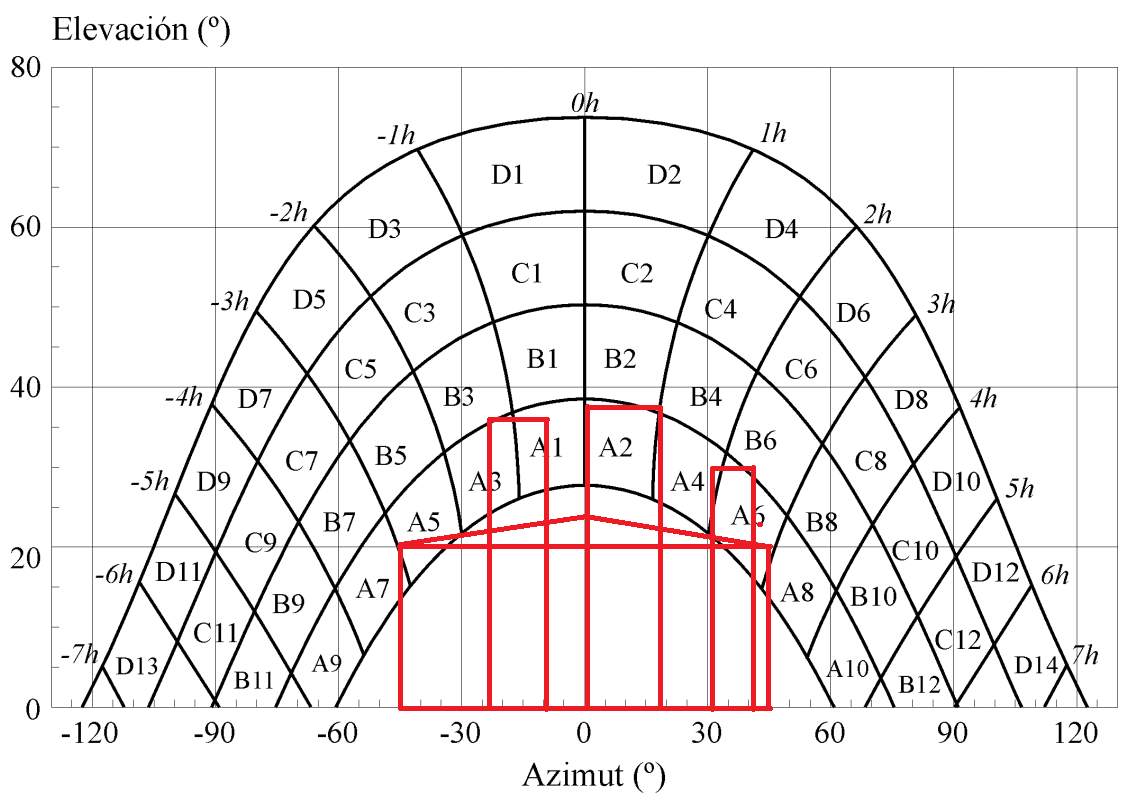
\includegraphics[scale=0.45]{images/o2.png}
\end{center}
\caption{Mapa d'ombres}
\label{fig: ombres}
\end{figure}

\noindent Degut a la inclinació i orientació de les plaques es fa servir la taula 5-A de l'IDAE, per tal de determinar el factor d'ombrejat (FS). Segons l'IDAE cal identificar si cada casella té un 0\%, un 25\%, un 50\%, un 75\% o un 100\% de la seva superfície coberta.\\
\newline La Taula \ref{tab:ombres} mostra el percentatge de superfície de cada casella, el valor de pèrdua tabulat de l'IDAE i la pèrdua que ocasiona cada casella. Així, es dona un total, el factor d'ombrejat (FS).
\begin{table}[H]
\small
  \centering
    \begin{tabular} {|l|r|r|r|}
 \hline  
 \multicolumn{1}{|l|}{Casella} &  \multicolumn{1}{r|}{Factor de superfície} &  \multicolumn{1}{r|}{Sombrejat casella al 100\%} &  \multicolumn{1}{r|}{Sombrejat casella} \\ \hline \hline
A5 & 0,25 & 1,84 & 0,46 \\ \hline
A3 & 0,5 & 2,70 & 1,35 \\ \hline
A1 & 0,5 & 3,15 & 1,58 \\ \hline
A2 & 1,0 & 3,17 & 3,17 \\ \hline
A6 & 0,75 & 1,79 & 1,34 \\ \hline \hline
Total & \multicolumn{3}{r|}{7,90} \\ \hline

    \end{tabular}%
    \caption{Sombrejats}
    \label{tab:ombres}
%\caption{Estances de l'habitatge unifamiliar}
\end{table}%

\noindent El total de 7,9\% entra dins els marges que marca l'IDAE, el qual indica que per instal·lacions de propòsit general el màxim per ombres és del 10\%.\\
\newline El factor d'ombrejat (FS) ve donat per l'Equació \ref{fs}.
\begin{equation} \label{fs}
FS = 1-Perdues \ per \ ombrejat
\end{equation}

\noindent El factor d'ombrejat val 0,921. Per tant, el total d'energia generada al cap de l'any baixa a 4.768 kWh.\\
\newline El factor d'irradiació és 1 perquè es pren l'angle òptim d'inclinació i l'angle d'orientació coincideix amb el sud.

% Per tal de determinar els panells solars escollits, abans necessitem conèixer la radiació que incideix sobre la teulada al llarg de l'any. Per fer-ho es consulta un servei web anomenat Photovoltaic Geographical Information System, de la Comissió Europea. El servei determina que, donades les coordenades de l'habitatge, el més òptim és inclinar les plaques amb un angle de 38$^\circ$ respecte la horitzontal i un angle de -3$^\circ$ respecte l'Azimut.

\section{Panell solar escollit}
El panell solar proposat s'anomena GCL-P6/72. Segons el fabricant és d'alta eficiència ja que pot arribar a tenir un 17\% de rendiment. La seva potència màxima, o potència de pic, és de 330 W. El fabricant indica que el rendiment dels panells disminueix de forma lineal al llarg del temps; al cap de 25 anys s'espera un rendiment d'un 80,7\%.\\
\newline Cal dir que aquests 330 W es poden haver aconseguit en condicions idònies que només es donen al laboratori. El mateix fabricant ens indica que per una irradiació de 800 W/$m^2$ la potència màxima és de 237,71 W.\\
\newline A continuació, a la Taula \ref{tab:panell_ideal}, s'indiquen les característiques elèctriques del panell en condicions idònies, per les quals es dona la potència de 330 W.

\begin{table}[H]
\small
  \centering
    \begin{tabular} {|l|r|}
 \hline  
 \multicolumn{1}{|l|}{Característica del panell GLC-P6/72 330 W, condicions ideals} &  \multicolumn{1}{r|}{Valor} \\ \hline \hline
	Potència màxima ($P_{max}$) & 330,00 W \\ \hline
	Tensió a la potència màxima ($V_m$) & 37,80 V \\ \hline
	Intensitat a la potència màxima ($I_m$) & 8,73 A \\ \hline
	Tensió de circuit obert ($V_{oc}$) & 46,20 V \\ \hline
	Corrent de curtcircuit ($I_{sc}$) & 9,33 A \\ \hline
	Eficiència & 17,00 \% \\ \hline
    \end{tabular}%
    \caption{Dades del panell amb irradiació de 1.000 W/$m^2$ i 25 C$^\circ$ de tempratura ambient}
    \label{tab:panell_ideal}
%\caption{Estances de l'habitatge unifamiliar}
\end{table}%

\noindent En condicions més comunes i no tan ideals la potència disminueix considerablement, com s'indica a la Taula \ref{tab:panell_habitual}.\\
\newline Després de consultar a Internet s'observa que a la zona geogràfica en què es pretén instal·lar les plaques la irradiació pot prendre valors de l'ordre de 800 W/$m^2$ com a màxim. Rebre 1.000 W/$m^2$ no seria gens comú.\\
\newline El mes de novembre, per exemple els pics d'irradiació que es reben són d'uns 600 W/$m^2$.

\begin{table}[H]
\small
  \centering
    \begin{tabular} {|l|r|}
 \hline  
 \multicolumn{1}{|l|}{Característica del panell GLC-P6/72 330 W, condicions no ideals} &  \multicolumn{1}{r|}{Valor} \\ \hline \hline
	Potència màxima ($P_{max}$) & 237,71 W \\ \hline
	Tensió a la potència màxima ($V_m$) & 34,50 V \\ \hline
	Intensitat a la potència màxima ($I_m$) & 6,89 A \\ \hline
	Tensió de circuit obert ($V_{oc}$) & 42,90 V \\ \hline
	Corrent de curtcircuit ($I_{sc}$)& 7,58 A \\ \hline

    \end{tabular}%
    \caption{Dades del panell amb irradiació de 800 W/$m^2$ i 20 C$^\circ$ de tempratura ambient}
    \label{tab:panell_habitual}
%\caption{Estances de l'habitatge unifamiliar}
\end{table}%

\noindent Un altre punt a destacar de la irradiació és que aquesta se sol donar en termes d'energia al cap del dia i no pas de potències. De totes maneres, se seguirà parlant de potències ja que és més pràctic. No s'ha d'oblidar, però, que aquesta potència de 800 W/$m^2$ només es pot donar a l'estiu i en moments de molta irradiació. En les demés hores aquesta potència serà molt menor.

%comentar com es decideix la potència que fa falta
%https://assets.leroymerlin.es/is/content/lmes/82165089-0170q-es/mod-fotovoltaico-gcl-330w.pdf


\section{Associació de plaques} %passar model i tal a annex?
Es decideix associar les plaques amb dues branques de 5 plaques per branca, de manera que es combina l'associació sèrie i paral·lel a la vegada. Per entendre millor aquest apartat es considera important conèixer el model dels panells solars, indicat a la Figura \ref{fig:model}.
\begin{figure}[H]
\begin{center}
\begin{tikzpicture} %http://www.texample.net/media/tikz/examples/TEX/power-electronics-rectifier.tex
    \draw
	(0,0)
	to [I=, l=$I_{PV}$] ++ (0,4)
	(2,4)
	to [D] ++(0,-4)
	(4,0)
	to[R=$R_{sh}$] ++(0,4)

    (0,0) to[short, -o] (7,0)
    (0,4) to[short, current/distance=0.5] (4.5,4)
    to[R=$R_{s}$] (5.5,4)
    to[short, i=$I_{out}$, -o] (7,4)
    
        (8,4)
        to[open, v^=$V_{out}$] ++(0,-4)
;
\end{tikzpicture}
\end{center}
\caption{Model d'un panell solar fotovoltaic}
\label{fig:model}
\end{figure}

\noindent $I_{PV}$: corrent que lliura el mòdul.\\
$R_{sh}$: resistència en paral·lel del panell.\\
$R_{s}$: resistència de contacte del connexionat del panell.\\
$I_{out}$: corrent de sortida.\\
$V_{out}$: tensió de sortida.\\
% 
\newline La corba característica $V_{out}$-$I_{out}$ dels panells solars s'obté d'aquest model i dona una intensitat lineal per un gran rang de tensions de sortida. Per altes tensions de sortida la intensitat de sortida és bastant petita. L'inversor intenta treballar en el punt de màxima potència, anomenat MPPT.\\
\newline Les corbes del panell segons el fabricant són les indicades a la Figura \ref{fig:vi}.
\begin{figure}[H]
\begin{center}
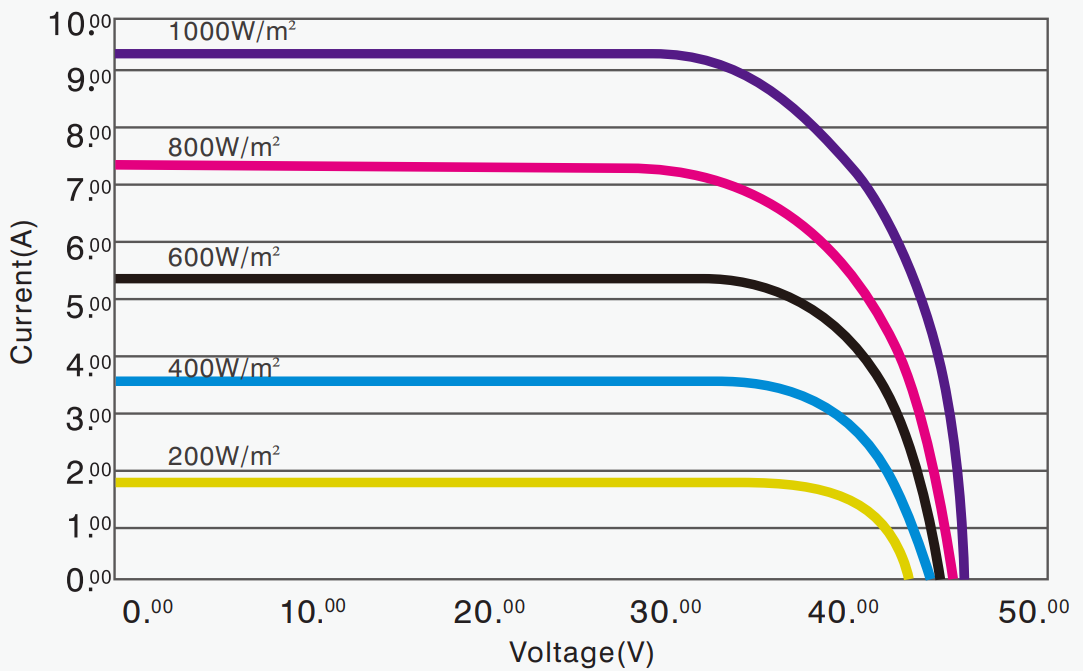
\includegraphics[scale=0.3]{images/corba.png}
\end{center}
\caption{Corbes V-I GLC-P6/72 330 W}
\label{fig:vi}
\end{figure}


\noindent Al connectar diversos panells en sèrie pot passar que algun panell consumeixi energia. Això és molt notori quan hi ha ombres, ja que a algunes plaques els incideix el Sol i lliuren una quantitat considerable d'intensitat mentre que les que estan a l'ombra donen molta menys intensitat. Com que estan connectades en sèrie, la intensitat ha de ser la mateixa. A la placa ombrejada, per tant, li passarà molta intensitat a través de $R_{sh}$. Aquesta resistència té un valor considerable. L'hi poden passar uns quants amperes i pot dissipar potències elevades.\\
\newline En cap cas interessa que un panell consumeixi energia enlloc de generar-ne. Com ja s'ha comentat, a la casa objecte d'aquest projecte s'ha observat que és habitual que es projectin ombres a la teulada, ja sigui pels alts arbres que hi ha properament o per les cases de més alçada que la del projecte.\\
\newline Per solucionar el problema una solució tradicional ha estat connectar díodes en paral·lel als terminals de les plaques. L'inconvenient és que aquests díodes tenen una caiguda de tensió de 0,7 V o 0,4 V si són díodes Schottky. Per una intensitat de branca de 7 A, que es podria donar per les plaques escollides, i considerant que múltiples plaques podrien estar ombrejades, es dissiparia una potència petita però considerable. A més, s'escalfarien els díodes. Aquests díodes es troben dins una petita caixa; l'escalfament els pot arribar a deteriorar i disminuir la robustesa de la instal·lació.\\
\newline Es decideix escollir un díode SM74611, o com diu el fabricant, un díode de derivació intel·ligent. De fet, se'n connectaran sis a cada placa.\\
\newline El panell GLC-P6/72 330 W té 6 files de 12 cel·les cadascuna. S'opta per col·locar un díode en paral·lel amb cada fila. Així, pot haver-hi alguna cel·la ombrejada però la resta del panell pot seguir generant energia.\\
\newline Els díodes SM74611 tenen una caiguda de tensió de 26 mV o menys a 7 A. Es pot afirmar que d'aquesta manera la pèrdua d'energia és mínima. \\
\newline El cost d'un díode és del 2\% aproximadament respecte el del panell.\\
%
%
\newline Un cops justificats els díodes, es poden fer els càlculs per conèixer la tensió i la intensitat màximes de sortides de la instal·lació fotovoltaica a partir de la tensió de circuit obert i a partir de la intensitat de curtcircuit. Aquestes dades es mostren a la Taula \ref{tab:maxs}.

\begin{table}[H]
\small
  \centering
    \begin{tabular} {|l|r|}
 \hline  
 \multicolumn{1}{|c|}{Característica} &  \multicolumn{1}{c|}{Valor} \\ \hline \hline
	Tensió màxima ($V_{max}$) & 256,87 V \\ \hline
	Intensitat màxima per branca & 9,56 A \\ \hline
    \end{tabular}%
%    \caption{Màxims de l'associació sèrie dels panells}
%\caption{Estances de l'habitatge unifamiliar}
\caption{Paràmetres màxims resultants de l'associació de plaques}
\label{tab:maxs}
\end{table}%

\noindent S'ha tingut en compte l'efecte de la temperatura. El fabricant dona uns factors per calcular els pitjors casos. A l'annex de càlculs es detallen.
%Díode SM74611
%http://www.ti.com/lit/ds/symlink/sm74611.pdf

\section{Inversor}

L'inversor escollit és un FRONIUS Primo 3.0-1. És costós en comparació a altres equips amb la mateixa funcionalitat però alhora molt fiable.\\
\newline Seguidament s'adjunta la Taula \ref{tab:inversor} amb algunes de les característiques més rellevants de l'inversor. L'equip és adient per la instal·lació de plaques i l'associació d'aquestes que es proposa. En cap cas se superen els màxims que fixa el fabricant de l'inversor. La potència del Fronius Primo 3.0-1 és correcta per la potència màxima que ens poden donar els panells fotovoltaics.
\begin{table}[H]
\small
  \centering
    \begin{tabular} {|l|r|} \hline
  \multicolumn{1}{|c|}{Característica} &  \multicolumn{1}{c|}{Valor}\\ \hline \hline
	Màxima corrent d'entrada ($I_{dc \ max}$) & 12 / 12 A \\ \hline
	Màxima corrent de curtcircuit & 18 / 18 A \\ \hline
	Rang màxim de tensió d'entrada CC ($U_{cc \ min}$ - $U_{cc \ max}$) & 80 - 1.000 V \\ \hline
	Tensió mínima de posada en marxa ($U_{dc \ arranc}$) & 80 V \\ \hline
	Nombre d'entrades CC & 2 + 2 \\ \hline
	Potència nominal AC ($P_{ac,r}$) & 3.000 W \\ \hline
	Acoblament a la xarxa ($U_{ac,r}$) & 1 NPE 230 V \\ \hline
	
    \end{tabular}%
  \label{tab:addlabel}%
  \caption{Característiques de l'inversor FRONIUS Primo 3.0-1}
  \label{tab:inversor}
 \end{table}%

\noindent Per començar a funcionar l'inversor necessita un mínim de 80 V. Si de dia un o dos panells estan ombrejats i la resta no, l'inversor pot seguir funcionant i lliurant energia.\\
\newline Els rendiments de l'inversor són molt elevats, per un gran rang de treball el rendiment és del 95\% o més. En cap cas el rendiment baixa del 80\%.\\
\newline El fabricant indica que l'inversor intenta donar sempre la màxima potència mitjançant el seu sistema de Dynamic Peak Manager, això vol dir que adapta la seva impedància per fer que el producte de tensió i intensitat sigui màxim.\\
\newline Aquest inversor és fàcil de muntar gràcies a què es pot desmuntar en dues parts: la fixa que va a la paret i és on es realitzen les connexions i la de potència, que pesa 21,5 kg. Primer es munta la part fixa, es realitzen les connexions, i després s'acobla la part de potència.\\
\newline Fronius indica que el Primo 3.0-1 és un equip pensat pel futur, per xarxes elèctriques intel·ligents. Hi ha la possibilitat de comunicar l'inversor per interfícies molt diverses com Modbus RTU, Fronius Solar API, Ethernet...\\
\newline S'opta per connectar l'inversor a Internet mitjançant un cable Ethernet. D'aquesta manera el client podrà visualitzar la generació d'energia elèctrica dels seus panells. La web que ofereix Fronius és entenedora i fàcil d'utilitzar.\\
\newline Gràcies a la web de Fronius i a la web que s'explica al següents capítols el client podrà visualitzar dades dels panells i tenir una molt bona idea de com estan funcionant.\\
\newline L'inversor donarà les dades de tensió, intensitat i potència generada, però no pot saber com està treballant cada panell. Per això hi ha la placa electrònica, la qual llegirà les tensions de cada panell, amb les quals l'usuari podrà determinar si els panells estan ombrejats, curtcircuitats o en funcionament normal.




\clearpage


% Table generated by Excel2LaTeX from sheet 'Hoja1'
%\begin{table}[H]
%  \centering
%    \begin{tabularx} {\textwidth} {|X|r|} \hline
%  \multicolumn{1}{|c|}{Descripció} &  \multicolumn{1}{c|}{Quantitat}\\ \hline \hline
%
 %   Placa GLC 330 W & 10 \\ \hline
%    Inversor FRONIUS Primo 3.0-1 Light 3kW & 1 \\ \hline
%    Metres cable Ethernet RJ-45 CAT 8 & 10 \\ \hline
%    Metres cable 4 m$m^2$ PVC & 45 \\ \hline
 %   Metres cable 1,5 m$m^2$ PVC & 100 \\ \hline
 %   Punteres Enghofer E 4-10, 4 m$m^2$, 10 mm & 20 \\ \hline
 %   Punteres Enghofer E 1.5-10 1,5 m$m^2$ 10 mm & 12 \\ \hline
 %   Cinta aïllant 10 m 1,6 cm & 3 \\ \hline
 %   Caixa estanca Solera CONS 100x100x55 mm & 2 \\ \hline
  %  Canal Euroquint 25,16 mm 1,5 metres & 20 \\ \hline
%    Curva canal VECAMCO & 10 \\ \hline
%    Paquet de 50 brides 200x2,6  mm & 2 \\ \hline
%    Regleta nylon 12 pols 16 mm & 4 \\ \hline
%    Premsaestopes M12 & 10 \\ \hline
%    Cargol autoroscant M4 16 mm & 12 \\ \hline
%    Tacs Fischer 072095 nylon 6x50 mm & 50 \\ \hline
%    Díode SM74611KTTR & 10 \\ \hline
%            Hores enginyer & 1 \\ \hline
%    Hores oficial de primera & 12 \\ \hline
%    Hores oficial de segona & 12 \\ \hline
%    \end{tabularx}%
%  \label{tab:addlabel}%
% \end{table}%

%\chapter{\uppercase{Inversor}}
%Fronius primo 3.0-1, %https://www.fronius.com/es-es/spain/energia-solar/productos/sector-dom%C3%A9stico/inversor/fronius-primo/fronius-primo-3-0-1

L'inversor escollit és un FRONIUS Primo 3.0-1. És costós en comparació a altres inversors però alhora molt fiable. Permet connectar-lo per TCP-IP a la xarxa d'Internet de la casa i així poder consultar en tot moment la quantitat d'energia que la instal·lació de panells solars fotovoltaics genera.\\
Seguidament s'adjunta una taula amb algunes de les característiques més rellevants de l'inversor.
\begin{table}[H]
  \centering
    \begin{tabular} {|l|r|} \hline
  \multicolumn{1}{|c|}{Característica} &  \multicolumn{1}{c|}{Valor}\\ \hline \hline
	Màxima corrent d'entrada ($I_{dc \ max}$) & 12 / 12 A \\ \hline
	Màxima corrent de curtcircuit & 18 / 18 A \\ \hline
	Rang màxim de tensió d'entrada CC ($U_{cc \ min}$ - $U_{cc \ max}$) & 80 - 1.000 V \\ \hline
	Tensió mínima de posada en marxa ($U_{dc \ arranc}$) & 80 V \\ \hline
	Nombre d'entrades CC & 2 + 2 \\ \hline
	Potència nominal AC ($P_{ac,r}$) & 3.000 W \\ \hline
	Acoblament a la xarxa ($U_{ac,r}$) & 1 NPE 230 V \\ \hline
	
    \end{tabular}%
  \label{tab:addlabel}%
  \caption{Característiques de l'inversor FRONIUS Primo 3.0-1}
 \end{table}%

\noindent L'inversor és adient per la instal·lació de plaques i l'associació d'aquestes que es proposa. En cap cas se superen els màxims que fixa el fabricant de l'inversor. La potència de l'inversor és correcta per la potència màxima que ens poden donar els panells fotovoltaics. Per començar a funcionar l'inversor necessita un mínim de 80 V. Si de dia un o dos panells estan ombrejats i la resta no l'inversor pot seguir funcionant i lliurant energia.\\
\newline Els rendiments de l'inversor són molt elevats, per un gran rang de treball el rendiment és del 95 \% o més. En cap cas el rendiment baixa del 80 \%.\\
\newline El fabricant indica que l'inversor intenta donar sempre la màxima potència mitjançant el seu sistema de Dynamic Peak Manager.\\
\newline Fronius permet connectar els seus inversors a Internet amb cable d'Ethernet i amb una aplicació web poder consultar l'energia que han generat i que estan generant les plaques. La interfície és simple i entenedora.\\
\newline Aquest inversor és fàcil de muntar gràcies a què es pot desmuntar en dues parts: la fixa que va a la paret i és on es realitzen les connexions i la de potència, que pesa bastant. Primer es munta la part fixa, es realitzen les connexions, i després s'acobla la part de potència.\\
\newline Fronius indica que el Primo 3.0-1 és un equip pensat pel futur, per xarxes elèctriques intel·ligents. Hi ha la possibilitat de comunicar l'inversor per interfícies molt diverses com Modbus RTU, Fronius Solar API, Ethernet...



\clearpage


% Table generated by Excel2LaTeX from sheet 'Hoja1'
%\begin{table}[H]
%  \centering
%    \begin{tabularx} {\textwidth} {|X|r|} \hline
%  \multicolumn{1}{|c|}{Descripció} &  \multicolumn{1}{c|}{Quantitat}\\ \hline \hline
%
 %   Placa GLC 330 W & 10 \\ \hline
%    Inversor FRONIUS Primo 3.0-1 Light 3kW & 1 \\ \hline
%    Metres cable Ethernet RJ-45 CAT 8 & 10 \\ \hline
%    Metres cable 4 m$m^2$ PVC & 45 \\ \hline
 %   Metres cable 1,5 m$m^2$ PVC & 100 \\ \hline
 %   Punteres Enghofer E 4-10, 4 m$m^2$, 10 mm & 20 \\ \hline
 %   Punteres Enghofer E 1.5-10 1,5 m$m^2$ 10 mm & 12 \\ \hline
 %   Cinta aïllant 10 m 1,6 cm & 3 \\ \hline
 %   Caixa estanca Solera CONS 100x100x55 mm & 2 \\ \hline
  %  Canal Euroquint 25,16 mm 1,5 metres & 20 \\ \hline
%    Curva canal VECAMCO & 10 \\ \hline
%    Paquet de 50 brides 200x2,6  mm & 2 \\ \hline
%    Regleta nylon 12 pols 16 mm & 4 \\ \hline
%    Premsaestopes M12 & 10 \\ \hline
%    Cargol autoroscant M4 16 mm & 12 \\ \hline
%    Tacs Fischer 072095 nylon 6x50 mm & 50 \\ \hline
%    Díode SM74611KTTR & 10 \\ \hline
%            Hores enginyer & 1 \\ \hline
%    Hores oficial de primera & 12 \\ \hline
%    Hores oficial de segona & 12 \\ \hline
%    \end{tabularx}%
%  \label{tab:addlabel}%
% \end{table}%

\chapter{\uppercase{Instal·lació elèctrica}}
És d'especial importància dimensionar correctament la instal·lació elèctrica dels panells fotovoltaics per tal de complir amb la ITC-BT-40 que tracta sobre instal·lacions generadores de baixa tensió. A més, cal protegir les línies amb les proteccions adients per tal d'evitar malmetre la instal·lació.

\section{Línies elèctriques de la instal·lació fotovoltaica}
La instal·lació elèctrica de la casa s'acull al model d'autoconsum amb compensació d'excedents. Això vol dir que els excedents d'energia, que es lliuren a la xarxa, es paguen a un preu menor al preu de l'energia que consumeix l'habitatge de la xarxa elèctrica. En cap cas, però, el client rebrà diners a cap de mes.\\
\newline A continuació, a la Taula \ref{tab:linies}, s'exposen les diferents línies de què disposa la instal·lació i la longitud més gran de cadascuna. Recordem que a l'inversor li arriben dos parells de cables, cada parell és d'una branca de 5 panells fotovoltaics en sèrie amb els seus díodes com a protecció.

\begin{table}[H]
\small
  \centering
    \begin{tabular} {|l|l|r|} \hline
  \multicolumn{1}{|l|}{Línia} &  \multicolumn{1}{l|}{Descripció} & \multicolumn{1}{c|}{Longitud (m)} \\ \hline \hline
L1 & Connexionat entre els panells solars & 10 \\ \hline
L2 & Connexionat de la branca 1 a l'inversor & 30 \\ \hline
L3 & Connexionat de la branca 2 a l'inversor & 19 \\ \hline
L4 & Connexionat de l'inversor al QGPC & 6 \\ \hline
L5 & Connexionat dels panells fotovoltaics a la placa electrònica & 21 \\ \hline
	
    \end{tabular}%
  \label{tab:addlabel}%
  \caption{Línies de la instal·lació fotovoltaica}
  \label{tab:linies}
 \end{table}%

\noindent La línia de connexionat entre els panells està formada per cables de baixa longitud que sumen els metres indicats a la taula. Hi ha una línia de connexionat dels panells a l'inversor per cada branca. Aquestes línies estan formades per un parell de cables de longituds diferents, i que sumen l'indicat a la taula. La connexió de l'inversor al QGPC es fa amb un parell de cables de la mateix longitud. Hi ha múltiples línies de connexionat dels panells fotovoltaics a la placa electrònica, la línia més llarga té la longitud indicada.\\
\newline Totes les línies són de cables flexibles de coure amb recobriment no propagador d'incendis i opacitat reduïda. Les línies 1, 2 i 4 tenen conductors amb recobriment contra la radiació directa del Sol. La línia 3 usa un cable comú amb recobriment PVC.


\section{Secció dels conductors}
%revisar tubs
Les seccions dels conductors estan calculades per complir amb el REBT. Es detallen els càlculs a l'annex de càlculs. Les seccions proposades es mostren a la Taula \ref{tab:eccions}.
\begin{table}[H]
\small
\begin{center}
 \begin{tabu} to \textwidth {|X[0.4, l]|X[2, l]|X[0.8, r]|X[0.6 , r]|X[0.6 , r]|}%{X | c c c} 
 \hline
 Línia & Descripció & Distància màxima (m) & Seccions ($mm^{2}$) & Diàmetre tub (mm)\\
 \hline \hline 

L1 & Connexionat entre els panells solars &  10 & 2x4 & 16 \\ \hline
L2 & Connexionat de la branca 1 a l'inversor & 30 & 2x10 & 20 \\ \hline 
L3 & Connexionat de la branca 2 a l'inversor  & 19 & 2x6 & 16 \\ \hline 
L4 & Connexionat de l'inversor al QGPC  & 6 & 2x4 + 4 & 25 \\ \hline
L5 & Connexionat dels panells fotovoltaics a la placa electrònica & 21 & 2x1,5 & 32 \\ \hline 

 \end{tabu}
 \caption{Seccions de les línies}
 \label{tab:eccions}
\end{center}
\end{table}

%detallar

\section{Quadre elèctric}
El quadre elèctric de la instal·lació fotovoltaica es troba a l'habitació on hi ha l'inversor i la placa electrònica. Aquesta habitació està situada sota teulada. Al pis de sota, a la planta baixa, hi ha el QGPC.\\
\newline La caixa del petit quadre elèctric que s'instal·larà és el model VE106F, amb un grau IP65.\\
\newline La protecció contra sobreintensitats, situada a la sortida de l'inversor, es mostra a la Taula \ref{tab:sobrei}. S'ha calculat a partir de la tensió de sortida de l'inversor, que és de 230 V, i amb la potència màxima de la instal·lació fotovoltaica, de 3.300 W.

\begin{table}[H]
\small
\begin{center}
 \begin{tabu} to \textwidth {|X[0.4, l]|X[2, l]|X[0.8, r]|X[0.7 , r]|X[0.4 , r]|X[0.4 , r]|}%{X | c c c} 
 \hline
 Línia & Descripció & Intensitat màxima de la línia (A) & Intensitat nominal del PIA (A) & Classe & Pols\\
 \hline \hline 

% L1 & Connexionat entre els panells solars &  10,91 & 16 & C & 2 \\ \hline

L4 & Connexionat de l'inversor al QGPC  & 14,35 & 16 & C & 2 \\ \hline

 \end{tabu}
 \caption{Proteccions contra sobreintensitats}
 \label{tab:sobrei}
\end{center}
\end{table}
%
%
\noindent És necessari disposar d'algun interruptor per obrir els circuits dels panells solars. Es decideix fer-ho amb interruptors magnetotèrmics. La seva intensitat és superior a la de curtcircuit de les plaques. No cal protegir els panells solars contra sobreintensitats, en curtcircuit el seu màxim no supera els 10 A. Els conductors s'han dimensionat per aguantar aquesta intensitat de curtcircuit sense problemes. Els interruptors són els de la Taula \ref{tab:sobrei2}.
%
\begin{table}[H]
\small
\begin{center}
 \begin{tabu} to \textwidth {|X[0.4, l]|X[2, l]|X[0.8, r]|X[0.7 , r]|X[0.4 , r]|X[0.4 , r]|}%{X | c c c} 
 \hline
 Línia & Descripció & Intensitat màxima de la línia (A) & Intensitat nominal del PIA (A) & Classe & Pols\\
 \hline \hline 
L2 & Connexionat de la branca 1 a l'inversor & 9,56 & 16 & C & 2 \\ \hline 
L3 & Connexionat de la branca 2 a l'inversor  & 9,56 & 16 & C & 2 \\ \hline 

 \end{tabu}
 \caption{Interruptors}
 \label{tab:sobrei2}
\end{center}
\end{table}


%revisar
\noindent El dimensionament dels conductors es detalla a l'annex de càlculs, on es tenen en compte els factors de radiació, agrupament, escalfament i el factor de 1,25 que indica la ITC-BT-40. També es té en compte l'efecte de la temperatura sobre les variables dels panells.\\
\newline La protecció contra contactes indirectes ve donada per un diferencial de classe A de 30 mA de sensibilitat, situat a la sortida de l'inversor. Altres característiques s'indiquen a la Taula \ref{tab:ind}.
%

\begin{table}[H]
\small
\begin{center}
 \begin{tabu} to \textwidth {|X[0.3, l]|X[1, l]|X[0.8, r]|X[0.7 , r]|X[0.7 , r]|X[0.4 , r]|}%{X | c c c} 
 \hline
 Línia & Descripció & Intensitat nominal de la línia (A) & Sensibilitat (mA) & Intensitat nominal del diferencial (A) & Classe\\ \hline \hline 

L4 & Connexionat de l'inversor al QGPC  & 14,35 & 30 & 40 & A \\ \hline

 \end{tabu}
 \caption{Proteccions contra contactes indirectes}
 \label{tab:ind}
\end{center}
\end{table}

\noindent Totes les carcasses de les plaques solars, que són metàl·liques, han d'estar connectades al terra de la instal·lació elèctrica de la casa. La resistència de terra es considerarà correcta si la tensió de defecte en qualsevol punt de la casa és menor a 24 V.

\clearpage


% Table generated by Excel2LaTeX from sheet 'Hoja1'
%\begin{table}[H]
%  \centering
%    \begin{tabularx} {\textwidth} {|X|r|} \hline
%  \multicolumn{1}{|c|}{Descripció} &  \multicolumn{1}{c|}{Quantitat}\\ \hline \hline
%
 %   Placa GLC 330 W & 10 \\ \hline
%    Inversor FRONIUS Primo 3.0-1 Light 3kW & 1 \\ \hline
%    Metres cable Ethernet RJ-45 CAT 8 & 10 \\ \hline
%    Metres cable 4 m$m^2$ PVC & 45 \\ \hline
 %   Metres cable 1,5 m$m^2$ PVC & 100 \\ \hline
 %   Punteres Enghofer E 4-10, 4 m$m^2$, 10 mm & 20 \\ \hline
 %   Punteres Enghofer E 1.5-10 1,5 m$m^2$ 10 mm & 12 \\ \hline
 %   Cinta aïllant 10 m 1,6 cm & 3 \\ \hline
 %   Caixa estanca Solera CONS 100x100x55 mm & 2 \\ \hline
  %  Canal Euroquint 25,16 mm 1,5 metres & 20 \\ \hline
%    Curva canal VECAMCO & 10 \\ \hline
%    Paquet de 50 brides 200x2,6  mm & 2 \\ \hline
%    Regleta nylon 12 pols 16 mm & 4 \\ \hline
%    Premsaestopes M12 & 10 \\ \hline
%    Cargol autoroscant M4 16 mm & 12 \\ \hline
%    Tacs Fischer 072095 nylon 6x50 mm & 50 \\ \hline
%    Díode SM74611KTTR & 10 \\ \hline
%            Hores enginyer & 1 \\ \hline
%    Hores oficial de primera & 12 \\ \hline
%    Hores oficial de segona & 12 \\ \hline
%    \end{tabularx}%
%  \label{tab:addlabel}%
% \end{table}%

%\chapter{\uppercase{Quadre elèctric}}
El quadre elèctric de la instal·lació fotovoltaica es troba a l'habitació on hi ha l'inversor i la placa electrònica. Aquesta habitació es troba sota teulada. Al pis de sota, a la planta baixa, es troba el quadre principal (QGPC).\\
\newline El quadre elèctric disposa d'un parell de magnetotèrmics de 2 pols encarregats de protegir la instal·lació dels panells fotovoltaics i permetre desconnectar-los de l'inversor. També hi figura un magnetotèrmic que es troba entre l'inversor i el QGPC.\\
\newline La caixa d'aquest petit quadre elèctric és el model VE106F, amb un grau IP65.

%
%
%

\begin{table}[H]
\small
\begin{center}
 \begin{tabu} to \textwidth {|X[0.4, l]|X[2, l]|X[0.8, r]|X[0.7 , r]|X[0.4 , r]|X[0.4 , r]|}%{X | c c c} 
 \hline
 Línia & Descripció & Intensitat nominal de la línia (A) & Intensitat nominal del PIA (A) & Classe & Pols\\
 \hline \hline 

L1 & Connexionat entre els panells solars &  10,91 & 16 & C & 2 \\ \hline
L2 & Connexionat de la branca 1 a l'inversor & 10,91 & 16 & C & 2 \\ \hline 
L3 & Connexionat de la branca 2 a l'inversor  & 10,91 & 16 & C & 2 \\ \hline 
L4 & Connexionat de l'inversor al QGPC  & 14,35 & 16 & C & 1 \\ \hline

 \end{tabu}
 \caption{Proteccions contra sobreintensitats}
\end{center}
\end{table}


%revisar
\noindent Pel correcte dimensionament de les proteccions contra sobreintensitats s'ha tingut en compte el coeficient de 1,25 que marca el REBT per instal·lacions generadores d'energia. Les plaques com a màxim, en funcionament normal donaran 8,73 A, aplicant el factor estem parlant de 10,91 A.\\
\newline La protecció contra contactes indirectes és un diferencial de classe A de 30 mA de sensibilitat, situat a la sortida de l'inversor.
%

\begin{table}[H]
\small
\begin{center}
 \begin{tabu} to \textwidth {|X[0.3, l]|X[1, l]|X[0.8, r]|X[0.7 , r]|X[0.7 , r]|X[0.4 , r]|}%{X | c c c} 
 \hline
 Línia & Descripció & Intensitat nominal de la línia (A) & Sensibilitat (mA) & Intensitat nominal del diferencial (A) & Classe\\ \hline \hline 

L4 & Connexionat de l'inversor al QGPC  & 14,35 & 30 & 40 & A \\ \hline

 \end{tabu}
 \caption{Proteccions contra contactes indirectes}
\end{center}
\end{table}

\noindent Totes les carcasses de les plaques solars, que són metàl·liques, estan connectades a terra.



\clearpage


% Table generated by Excel2LaTeX from sheet 'Hoja1'
%\begin{table}[H]
%  \centering
%    \begin{tabularx} {\textwidth} {|X|r|} \hline
%  \multicolumn{1}{|c|}{Descripció} &  \multicolumn{1}{c|}{Quantitat}\\ \hline \hline
%
 %   Placa GLC 330 W & 10 \\ \hline
%    Inversor FRONIUS Primo 3.0-1 Light 3kW & 1 \\ \hline
%    Metres cable Ethernet RJ-45 CAT 8 & 10 \\ \hline
%    Metres cable 4 m$m^2$ PVC & 45 \\ \hline
 %   Metres cable 1,5 m$m^2$ PVC & 100 \\ \hline
 %   Punteres Enghofer E 4-10, 4 m$m^2$, 10 mm & 20 \\ \hline
 %   Punteres Enghofer E 1.5-10 1,5 m$m^2$ 10 mm & 12 \\ \hline
 %   Cinta aïllant 10 m 1,6 cm & 3 \\ \hline
 %   Caixa estanca Solera CONS 100x100x55 mm & 2 \\ \hline
  %  Canal Euroquint 25,16 mm 1,5 metres & 20 \\ \hline
%    Curva canal VECAMCO & 10 \\ \hline
%    Paquet de 50 brides 200x2,6  mm & 2 \\ \hline
%    Regleta nylon 12 pols 16 mm & 4 \\ \hline
%    Premsaestopes M12 & 10 \\ \hline
%    Cargol autoroscant M4 16 mm & 12 \\ \hline
%    Tacs Fischer 072095 nylon 6x50 mm & 50 \\ \hline
%    Díode SM74611KTTR & 10 \\ \hline
%            Hores enginyer & 1 \\ \hline
%    Hores oficial de primera & 12 \\ \hline
%    Hores oficial de segona & 12 \\ \hline
%    \end{tabularx}%
%  \label{tab:addlabel}%
% \end{table}%


\chapter{\uppercase{Placa electrònica d'adquisició de dades i comunicació}}
Tal com s'indica als objectius del projecte part del treball consisteix en desenvolupar una placa electrònica encarregada d'adquirir dades, en aquest cas de tensió, dels panells fotovoltaics.\\
\newline Es vol que aquestes dades siguin accessibles i per això s'ha optat per dotar la placa d'un component de comunicació Wi-Fi gràcies al qual es podrà visualitzar una pàgina web amb les dades mesurades.\\
\newline La placa disposa d'una part d'alimentació que s'encarrega d'adaptar les tensions als nivells correctes dels diversos components. Uns circuits d'instrumentació atenuen la tensió d'entrada i fan les restes per obtenir la diferència de tensió entre els dos terminals de cada panell. Es multiplexen les senyals i es llegeix el seu valor digital.

\section{Alimentació}
% Comentar com s'aliment placaa la. Afegir l'equip a amidaments i pressupost.
La placa dissenyada s'alimenta amb un cable Micro-USB el qual es connecta a un equip de potència format per un rectificador i un convertidor DC-DC reductor, o sigui, de tipus Buck. Aquest equip, que molta gent identificaria com un carregador de telèfon mòbil, entrega 5 V a la seva sortida i un màxim de 2 A.\\
\newline La placa electrònica dissenyada disposa d'un integrat SMD que converteix la tensió de 5 V a 3,3 V, anomenat SPX3819M5-L-3-3. Els operacionals van alimentats a 5 V. L'integrat de comunicacions i altres parts de la placa van alimentats amb 3,3 V.\\
\newline Algunes característiques del regulador són les indicades a la Taula \ref{tab:regulador}.
\begin{table}[H]
\small
\begin{center}
 \begin{tabular} {|l|r|}%{X | c c c} 
 \hline
 Característica & Valor \\
 \hline \hline 
Tensió de sortida & 3,3 V \\ \hline
Corrent màxim de sortida & 500 mA\\ \hline
Tensió mínima d'entrada & 2,5 V \\ \hline
Precisió de regulació de voltatge & 1\% \\ \hline
Tensió màxima d'entrada & 16 V \\ \hline
Corrent de repòs & 90 $\mu$A \\ \hline
Empaquetat & SOT-23-5 \\ \hline

 \end{tabular}
 \caption{Característiques del regulador de tensió SPX3819M5-L-3-3}
 \label{tab:regulador}
\end{center}
\end{table}
%\si\ohm

\noindent Pel que fa a la intensitat, la placa consumeix al voltant de 100 mA en funcionament normal. Pot arribar a consumir uns 200 mA en certs moments. El convertidor de tensió de 5 V a 3,3 V pot donar fins a 500 mA a la seva sortida, molt superior al màxim que pot necessitar la placa.\\
\newline L'esquema de connexionat del regulador és el de la Figura \ref{fig: circuit_reg}.
\begin{figure}[H]
\begin{center}
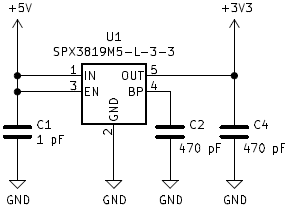
\includegraphics[scale=0.5]{images/regulador.png}
\end{center}
\caption{Regulador de tensió}
\label{fig: circuit_reg}

\end{figure}
\noindent El convertidor de tensió disposa de condensadors a l'entrada i a la sortida per tal de garantir una tensió el més constant possible, per bé que la recomanació del fabricant és connectar-ne només un a l'entrada. Si la sortida sol·licita un pic de corrent els condensadors el poden subministrar durant els instants en què el regulador encara no hagi reaccionat.\\
\newline Així, el dimensionament dels equips d'alimentació es considera correcte.

\section{Instrumentació}
% Insistir en la part d'instrumentació, posar equacions i indicar càlculs seguits
% Discutir per què s'ha escollit un OP AMP o un altre i així
La placa disposa d'una part d'instrumentació que s'encarrega d'adaptar les tensions dels panells solars fotovoltaics a les tensions amb què pot treballar el convertidor analògic digital. Interessa conèixer la diferència de tensió als terminals de cada placa. El circuit és l'indicat a la Figura \ref{fig:restador}.\\
\newline El primer que es fa és reduir la tensió considerablement mitjançant un divisor de tensió connectat a un seguidor de voltatge. El seguidor de voltatge és important tenir-lo per aïllar aquesta primera etapa de la resta. Les resistències es detallen a l'estat d'amidaments i al pressupost. El seu valor de potència màxima a dissipar és adient.\\
\newline El divisor de tensió ha de ser tal faci que a l'entrada no inversora la tensió sigui menor o igual a 3,5 V, tal com s'exposa més endavant.

\begin{figure}[H]
\begin{center}
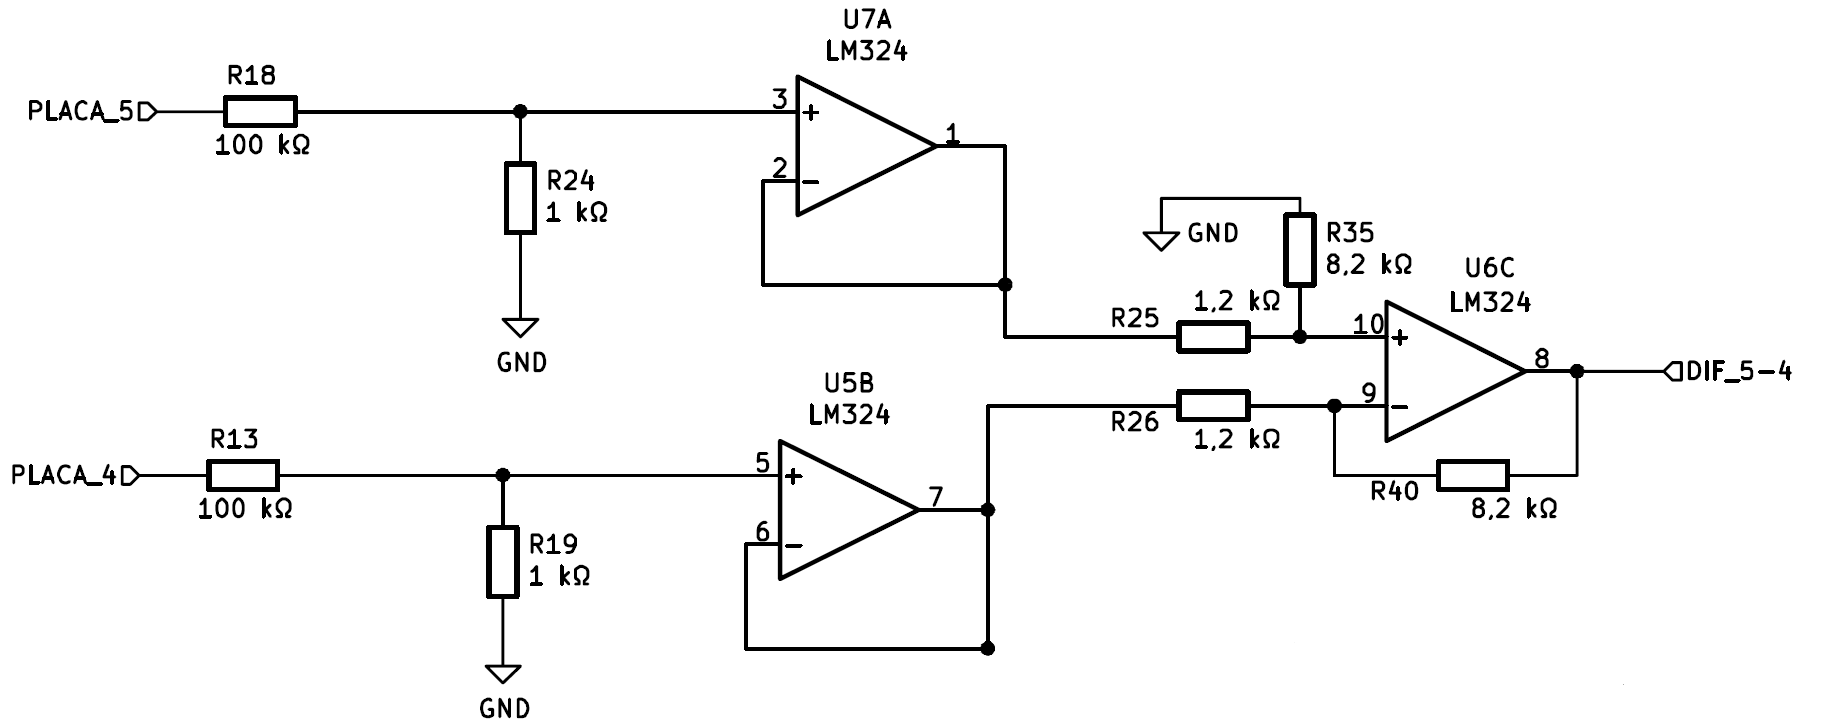
\includegraphics[scale=0.3]{images/restador.png}
\end{center}
\caption{Circuit atenuador i restador}
\label{fig:restador}
\end{figure}

\noindent El guany de la primera etapa és el de l'Equació \ref{guany1}.

\begin{equation} \label{guany1}
\Delta_{1}=\frac{R_{24}}{R_{24}+R_{18}}
\end{equation}

\noindent Seguidament s'utilitza un restador que alhora amplifica la tensió resultant. El fabricant de les plaques ens dona un màxim de tensió de 46,2 V que per efectes de la temperatura pot passar a valer 51,37 V. Tenim en compte aquesta tensió per dimensionar el restador. El circuit està dissenyat per aprofitar tot el rang del convertidor analògic digital.\\
\newline S'imposa que els parells següents de resistències siguin iguals, per simplificar els càlculs. La primera parella de resistències iguals són la de l'Equació \ref{r1}.

\begin{equation} \label{r1}
R_{25}=R_{26}
\end{equation}

\noindent I el mateix per l'altre parell, segons l'Equació \ref{r2}.
\begin{equation} \label{r2}
R_{35}=R_{40}
\end{equation}

\noindent Aleshores el guany de la segona etapa ve donat per l'Equació \ref{guany2}.

\begin{equation} \label{guany2}
\Delta_{2}=\frac{R_{35}}{R_{25}}
\end{equation}

\noindent Aquest guany és de 6,8. Amb tot això podem escriure la relació entre les dues entrades i la sortida del circuit mostrat. Ho indica l'Equació \ref{relacio}.
\begin{equation} \label{relacio}
V_{5-4} =  \left (V_5 - V_4  \right ) \Delta_{1} \Delta_{2} = 0,0677
\end{equation}


%
%
%
\noindent Els amplificadors operacions escollits són del model LM324. Són de baix cost i les seves prestacions són més que suficients per aquest cas en què es treballa amb senyals contínues. Algunes característiques s'indiquen a la Taula \ref{tab:lm324}.
\begin{table}[H]
\small
\begin{center}
 \begin{tabular} {|l|r|}%{X | c c c} 
 \hline
 Característica & Valor \\
 \hline \hline 
Guany unitari & 100 dB \\ \hline
Rang de tensió d'alimentació single supply & 3 V a 32 V \\ \hline
Tensió d'offset màxima & 2 mV \\ \hline
Rang de tensió de sortida & 0 V a $V_{cc}$-1,5 V \\ \hline
Corrent màxim de sortida en source & 40 mA \\ \hline

 \end{tabular}
 \caption{Característiques de l'amplificador operacional LM324}
 \label{tab:lm324}
\end{center}
\end{table}
%\si\ohm
%
\noindent El rang d'alimentació i el rang de tensió de sortida són dos paràmetres que s'han tingut molt en compte pel disseny. L'amplificador operacional LM324, tot i no ser Rail-to-Rail, l'alimentarem a 5 V i així tindrem sortides màximes de fins a 3,5 V, que és un nivell de tensió adequat per aquesta placa. El corrent de sortida i l'offset de tensió també són acceptables per l'aplicació.

\section{Multiplexor}

La placa que s'ha dissenyat disposa de l'integrat ESP-12E, que entre d'altres té una entrada analògica. Al tenir 10 senyals analògiques per llegir i una sola entrada analògica s'opta per utilitzar un multiplexor.\\
\newline Aquest multiplexor té 16 entrades, un pin per habilitar-lo, 4 pins per seleccionar quin canal llegir i una sola sortida.\\
\newline Tot i que els multiplexors són molt usats en electrònica digital, el fabricant ens indica que també està pensat per fer servir amb senyals analògiques, gràcies a la baixa resistència entre una entrada habilitada i la sortida.\\
\newline El multiplexor i la connexió de la sortida analògica al mòdul ESP-12E és la indicada a la Figura \ref{fig:mux}.\\
\newline Cal dir que aquesta imatge és una simplificació del circuit mostrat a plànols. S'han eliminat algunes connexions per fer la figura més entenedora.

\begin{figure}[H]
\begin{center}
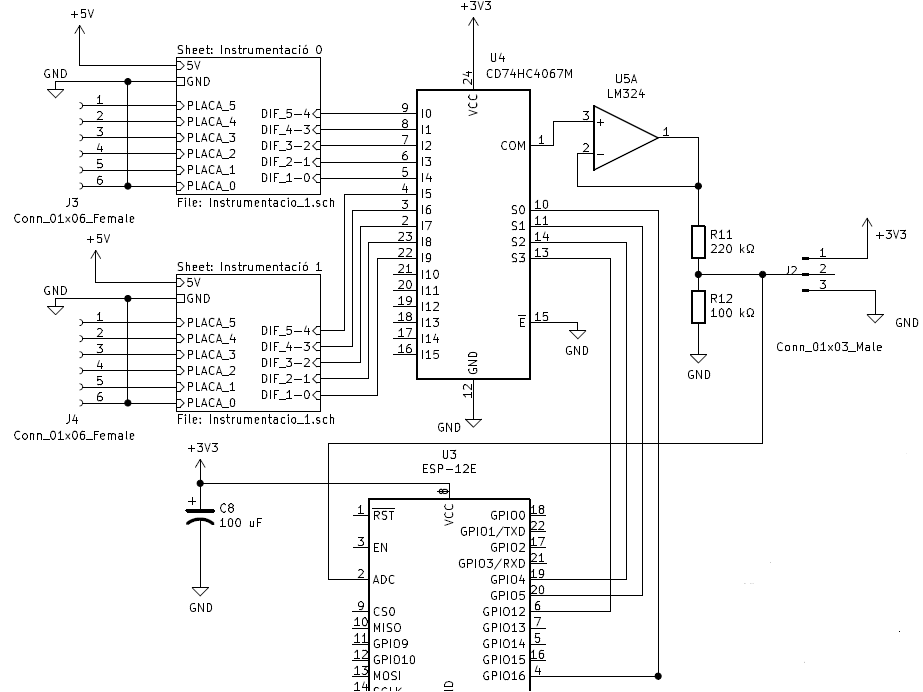
\includegraphics[scale=0.60]{images/mux.png}
\end{center}
\caption{Multiplexor i entrada digital}
\label{fig:mux}
\end{figure}

\noindent Les sortides dels circuits d'instrumentació són les entrades del multiplexor. La lògica és positiva. S0 és el bit de menys pes i S3 el de més pes. S'habilita el multiplexor connectant-lo a massa.\\
\newline Per la programació, no s'ha de confondre l'etiqueta del component ESP-12E amb el número de pin que es programarà. Això es pot visualitzar a la Taula \ref{tab:programacio_pins}.

\begin{table}[H]
\small
\begin{center}
 \begin{tabular} {|l|r|}%{X | c c c} 
 \hline
 GPIO & Número de pin a programar  \\ \hline \hline 
GPIO 12 & 6 \\ \hline
GPIO 4 & 2 \\ \hline
GPIO 5 & 1 \\ \hline
GPIO 16 & 0 \\ \hline
 \end{tabular}
 \caption{Relació entre les sortides i el seu número de pin a programar}
 \label{tab:programacio_pins}
\end{center}
\end{table}

\noindent Com s'indica a l'annex de programació, es programen els pins de caràcter general com a sortides per controlar el multiplexor.\\
\newline La taula de veritat és la de la Taula \ref{tab:veritat}.

\begin{table}[H]
\small
\begin{center}
 \begin{tabular} {|l|l|l|l|l|r|}%{X | c c c} 
 \hline
 CGPIO12 & GPIO4 & GPIO5 & GPIO16 & ~E & Sortida \\ \hline \hline 
 0 & 0 & 0 & 0 & 0 & 0\_DIF\_5-4 \\ \hline
 0 & 0 & 0 & 1 & 0 & 0\_DIF\_4-3 \\ \hline
 0 & 0 & 1 & 0 & 0 & 0\_DIF\_3-2 \\ \hline
 0 & 0 & 1 & 1 & 0 & 0\_DIF\_2-1 \\ \hline
 0 & 1 & 0 & 0 & 0 & 0\_DIF\_1-0 \\ \hline
 
 0 & 1 & 0 & 1 & 0 & 1\_DIF\_5-4 \\ \hline
 0 & 1 & 1 & 0 & 0 & 1\_DIF\_4-3 \\ \hline
 0 & 1 & 1 & 1 & 0 & 1\_DIF\_3-2 \\ \hline
 1 & 0 & 0 & 0 & 0 & 1\_DIF\_2-1 \\ \hline
 1 & 0 & 0 & 1 & 0 & 1\_DIF\_1-0 \\ \hline
 \end{tabular}
 \caption{Taula de veritat}
 \label{tab:veritat}
\end{center}
\end{table}

\noindent Algunes característiques del multiplexor són les de la Taula \ref{mux_ds}.
%
\begin{table}[H]
\small
\begin{center}
 \begin{tabular} {|l|r|}%{X | c c c} 
 \hline
 Característica & Valor \\
 \hline \hline 
Resistència ON, $V_{CC}$=4,5V & 70 \si\ohm \\ \hline
Rang de tensió d'alimentació & -0,5 V a 7 V \\ \hline
Temps de transició màxim & 1.000 ms \\ \hline
Corrent màxim de fuga a les entrades lògiques & 1 $\mu$A \\ \hline
Nivell lògic alt, $V_{CC}$=4,5V & 2 V \\ \hline
Nivell lògic baix, $V_{CC}$=4,5V & 0,8 V \\ \hline
 \end{tabular}
 \caption{Característiques del multiplexor CD74HC4067M}
 \label{mux_ds}
\end{center}
\end{table}



\noindent Hi ha un seguidor per tal d'aïllar les etapes i un divisor de tensió encarregat d'adaptar la tensió al conversor analògic digital, que té un màxim d'1 V. 


\section{Comunicació}
% Explicar els diferents blocs lògics de la placa
La placa electrònica dissenyada permet establir comunicació Wi-Fi de forma efectiva. L'integrat ESP-12E és un component molt popular que es basa en l'ESP8266. L'ESP-12E és un component que disposa d'una petita memòria on es bolca el programa, d'uns quants pins digitals de propòsit general, d'una entrada analògica i d'una antena impresa en circuit imprès, a més de l'ESP8266.\\
\newline El fabricant indica que es deixi una àrea lliure de coure sota l'antena per evitar interferències i problemes de comunicació.\\
\newline Tot i tenir una simple antena impresa en circuit imprès el rang de comunicació Wi-Fi és generós i suficient per l'aplicació que es desitja.\\
\newline Algunes característiques de l'ESP8266 venen donades a la Taula \ref{tab:ESP8266}.
\begin{table}[H]
\small
\begin{center}
 \begin{tabular} {|l|r|}%{X | c c c} 
 \hline
 Característica & Valor \\
 \hline \hline 
Certificació & Wi-Fi Alliance \\ \hline
Freqüència de treball & 2,4 GHz \\ \hline
Potència de l'emissor & 17 dBm \\ \hline
Llindar de potència del receptor & -75 dBm \\ \hline
Rang de tensió d'alimentació & 2,5 V a 3,6 V \\ \hline
Corrent en funcionament normal & 80 mA \\ \hline

 \end{tabular}
 \caption{Característiques de l'integrat de comunicació ESP-8266}
 \label{tab:ESP8266}
\end{center}
\end{table}
% \si\ohm

\noindent D'aquí la importància d'alimentar-lo amb 3,3 V enlloc dels 5 V que ens arriben al connector. Per això es fa servir el regulador de tensió. El consum del dispositiu no és molt elevat però és considerable, no seria viable tenir la placa amb una bateria.

\section{Circuit imprès}
% Questions de PCB, clearance i tal
S'ha dissenyat un PCB a doble cara que conté la part d'alimentació, la part d'instrumentació i la part de comunicació. Disposa dels connectors necessaris.\\
\newline Les pistes d'alimentació s'han fet més gruixudes que les de senyal digital. Les pistes de tensió de les plaques s'han fet una mica més gruixudes, tot i que la intensitat a través seu és petita. La separació d'una d'aquestes pistes amb la resta és generosa per evitar l'arc elèctric. A més, es preveu recobrir la placa amb una pel·lícula, cosa que disminuiria encara més el risc d'arc elèctric.\\
\newline La majoria de components són SMD. Solen ser més barats i ocupen molt menys espai en comparació als components que travessen la placa. Així, les dimensions finals de la placa són de 8,4 x 10 cm aproximadament.\\
\newline S'han seguit especificacions del fabricant pel disseny de la part de RF. Pel disseny de la part d'instrumentació s'ha tingut especial cura en utilitzar condensadors de desacoblament a les alimentacions dels integrats i situar-los prop d'aquests.\\
\newline La vista superior de com quedaria la placa és la de la Figura \ref{fig:3d_sup}.
\begin{figure}[H]
\begin{center}
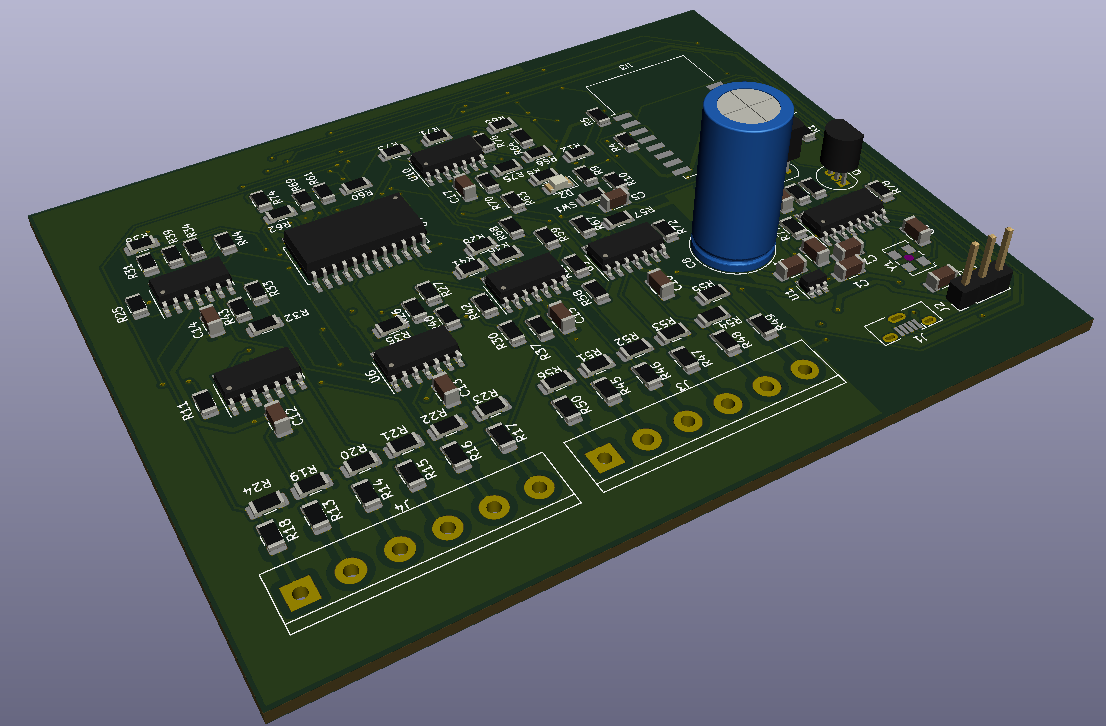
\includegraphics[scale=0.32]{images/3d_1.png}
\end{center}
\caption{Vista 3D de la cara superior de la placa}
\label{fig:3d_sup}
\end{figure}

\noindent Es pot observar com tots els amplificadors operacionals tenen un condensador molt proper; aquest condensador és el condensador de desacoblament. Els que he escollit son de 100 nF, un valor molt típic.\\
\newline No es disposa del model 3D dels connectors de les senyals dels panells solars, del connector micro USB i del component ESP-12E.\\
\newline Pel que fa a la cara inferior, aquesta es mostra a la Figura \ref{fig:inf}.

\begin{figure}[H]
\begin{center}
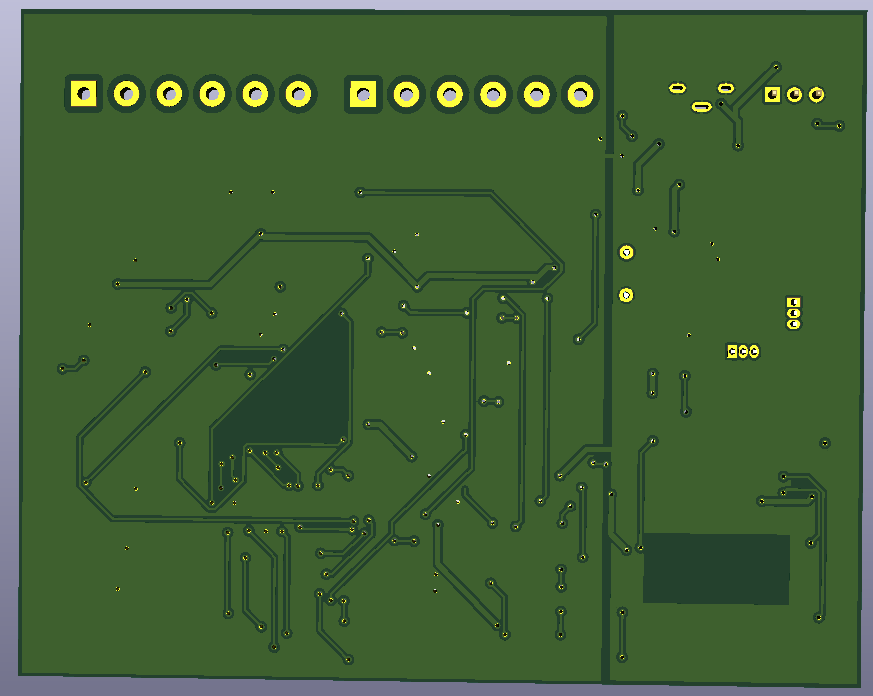
\includegraphics[scale=0.30]{images/3d_2.png}
\end{center}
\caption{Vista de la cara inferior de la placa}
\label{fig:inf}
\end{figure}
\noindent Els plans de massa es connecten per un petit conductor. D'aquesta manera el pla de massa digital està connectat al pla de massa de la part analògica del circuit i alhora es minimitza el soroll transmès de la part digital a l'analògica.


\clearpage


% Table generated by Excel2LaTeX from sheet 'Hoja1'
%\begin{table}[H]
%  \centering
%    \begin{tabularx} {\textwidth} {|X|r|} \hline
%  \multicolumn{1}{|c|}{Descripció} &  \multicolumn{1}{c|}{Quantitat}\\ \hline \hline
%
 %   Placa GLC 330 W & 10 \\ \hline
%    Inversor FRONIUS Primo 3.0-1 Light 3kW & 1 \\ \hline
%    Metres cable Ethernet RJ-45 CAT 8 & 10 \\ \hline
%    Metres cable 4 m$m^2$ PVC & 45 \\ \hline
 %   Metres cable 1,5 m$m^2$ PVC & 100 \\ \hline
 %   Punteres Enghofer E 4-10, 4 m$m^2$, 10 mm & 20 \\ \hline
 %   Punteres Enghofer E 1.5-10 1,5 m$m^2$ 10 mm & 12 \\ \hline
 %   Cinta aïllant 10 m 1,6 cm & 3 \\ \hline
 %   Caixa estanca Solera CONS 100x100x55 mm & 2 \\ \hline
  %  Canal Euroquint 25,16 mm 1,5 metres & 20 \\ \hline
%    Curva canal VECAMCO & 10 \\ \hline
%    Paquet de 50 brides 200x2,6  mm & 2 \\ \hline
%    Regleta nylon 12 pols 16 mm & 4 \\ \hline
%    Premsaestopes M12 & 10 \\ \hline
%    Cargol autoroscant M4 16 mm & 12 \\ \hline
%    Tacs Fischer 072095 nylon 6x50 mm & 50 \\ \hline
%    Díode SM74611KTTR & 10 \\ \hline
%            Hores enginyer & 1 \\ \hline
%    Hores oficial de primera & 12 \\ \hline
%    Hores oficial de segona & 12 \\ \hline
%    \end{tabularx}%
%  \label{tab:addlabel}%
% \end{table}%

%\chapter{\uppercase{Caixa}}




\clearpage


% Table generated by Excel2LaTeX from sheet 'Hoja1'
%\begin{table}[H]
%  \centering
%    \begin{tabularx} {\textwidth} {|X|r|} \hline
%  \multicolumn{1}{|c|}{Descripció} &  \multicolumn{1}{c|}{Quantitat}\\ \hline \hline
%
 %   Placa GLC 330 W & 10 \\ \hline
%    Inversor FRONIUS Primo 3.0-1 Light 3kW & 1 \\ \hline
%    Metres cable Ethernet RJ-45 CAT 8 & 10 \\ \hline
%    Metres cable 4 m$m^2$ PVC & 45 \\ \hline
 %   Metres cable 1,5 m$m^2$ PVC & 100 \\ \hline
 %   Punteres Enghofer E 4-10, 4 m$m^2$, 10 mm & 20 \\ \hline
 %   Punteres Enghofer E 1.5-10 1,5 m$m^2$ 10 mm & 12 \\ \hline
 %   Cinta aïllant 10 m 1,6 cm & 3 \\ \hline
 %   Caixa estanca Solera CONS 100x100x55 mm & 2 \\ \hline
  %  Canal Euroquint 25,16 mm 1,5 metres & 20 \\ \hline
%    Curva canal VECAMCO & 10 \\ \hline
%    Paquet de 50 brides 200x2,6  mm & 2 \\ \hline
%    Regleta nylon 12 pols 16 mm & 4 \\ \hline
%    Premsaestopes M12 & 10 \\ \hline
%    Cargol autoroscant M4 16 mm & 12 \\ \hline
%    Tacs Fischer 072095 nylon 6x50 mm & 50 \\ \hline
%    Díode SM74611KTTR & 10 \\ \hline
%            Hores enginyer & 1 \\ \hline
%    Hores oficial de primera & 12 \\ \hline
%    Hores oficial de segona & 12 \\ \hline
%    \end{tabularx}%
%  \label{tab:addlabel}%
% \end{table}%

\chapter{\uppercase{Programació}}
% Testejar cosetes i poder treure algun screenshot (?, o l'screen shot no fa falta?
% Adjuntar codi, aquí o en annex
S'ha desenvolupat un programa per adquirir correctament les senyals analògiques, calcular la tensions i mostrar-les en un parell de gràfiques en una web. Es porta un comptatge de temps per tal d'efectuar les lectures de tensió de forma periòdica. El programa mostra la web al client si aquest es connecta a l'adreça IP del dispositiu pel port 80, en aquest cas.
\section{Organigrama}
L'organigrama de la Figura \ref{fig:organigrama} és una forma simplificada d'explicar la solució adoptada. A l'annex de programa figura el codi complet.


% fill=blue!20, 
\tikzstyle{decision} = [diamond, draw, fill=orange!20, 
    text width=4.5em, text badly centered, node distance=3cm, inner sep=0pt]
\tikzstyle{block} = [rectangle, draw, fill=blue!10, 
    text width=5em, text centered, rounded corners, minimum height=4em]
\tikzstyle{line} = [draw, -latex']
\tikzstyle{cloud} = [draw, ellipse,fill=red!20, node distance=3cm,
    minimum height=2em]
    
\begin{figure}[H]
\begin{center}
\begin{tikzpicture}[node distance = 3cm, auto, scale=0.65, every node/.style={scale=0.65}]
    % Place nodes
    \node [block] (inici) {Inicialització};
    \node [block, below of=inici, node distance=3cm] (intent) {Intenta connexió Wi-Fi};
    \node [decision, below of=intent] (decide) {Dispositiu connectat via Wi-Fi?};
    \node [block, left of=decide, node distance=4cm] (delay) {Espera 500 ms};
        \node [decision, below of=decide, node distance=4cm] (wifii) {Client connectat?};
            \node [block, below of= wifii, node distance=3cm] (comprova) {Comprova temps};
            \node [block, right of=wifii, node distance=4cm] (webbb) {Mostra web};
    \node [decision, below of=comprova, node distance=3cm] (mesura) {Cal fer una mesura?};
    \node [decision, below of=mesura, node distance=4cm] (wifi) {Client connectat?};
    \node [block, right of=wifi, node distance=4cm] (guarda) {Mesura i guarda dades};
    \node [block, below of=wifi, node distance=3cm] (webb) {Mostra web};
    
        \node [ left of=wifi, node distance=4cm] (punt) {.};

    % Draw edges
    \path [line] (inici) -- (intent);
    \path [line] (intent) -- (decide);    
    \path [line] (decide) -- node [near start] {Sí}(wifii);    
    \path [line] (decide) -- node [near start] {No}(delay);
    

    \path [line] (comprova) -- (mesura); 
    \path [line] (mesura) -- node [near start] {No} (wifi); 
	\path [line] (mesura) -| node [near start] {Sí} (guarda);
	\path [line] (guarda) -- (wifi);
   \path [line] (wifi) -- node [near start] {Sí} (webb);
   
   \path [line] (webb) -| (punt);
   \path [line] (wifii) -- node [near start] {Sí} (webbb);
    \path [line] (wifii) -- node [near start] {No} (comprova);
 \path [line] (webbb) |-  (comprova);    
    
	\path [line] (wifi) -- node [near start] {No} (punt);
	\path [line] (punt) |- (comprova);   
	
    \path [line] (delay) |- (intent);
    
\end{tikzpicture}
\end{center}
\caption{Organigrama del codi}
\label{fig:organigrama}
\end{figure}

%\section{Explicació}
%
\noindent Quan s'inicia el programa el primer que es fa és inicialitzar variables i intentar connectar-se a la xarxa Wi-Fi de la qual s'ha definit la contrasenya i el nom, o més ben dit, l'SSID. Si el dispositiu és incapaç de connectar-se a la xarxa Wi-Fi ho segueix intentant cada mig segon.
\end{spacing}
\begin{spacing}{1}
\begin{lstlisting}[style=myArduino]
  // Ens connectem al Wi-Fi amb l'adreça i la contrasenya definits
  Serial.print("Connectant a: ");
  Serial.println(ssid); // Mostrem l'adreça del Wi-Fi
  WiFi.begin(ssid, password); // Iniciem la comunicació
  
  while (WiFi.status() != WL_CONNECTED) {
    delay(500);
    Serial.print("."); // Cada 0,5 s que passin sense connectar-se mostra un punt
  }
  
  // S'ha connectat
  Serial.println("");
  Serial.println("WiFi connectat");
  Serial.println("Adreça IP: ");
  Serial.println(WiFi.localIP());
  server.begin();
\end{lstlisting}

\end{spacing}
\begin{spacing}{1.5}

\noindent Un cop té connectivitat Wi-Fi mira si té algun client connectat, i en cas de què sigui així li mostra la web.\\
\newline Per defecte s'han emplenat els vectors de dades fictícies per tal de mostrar com es presenten les gràfiques  que es fan amb JavaScript. A mesura que passin les hores aquestes dades s'aniran sobreescrivint per dades reals. La resta de la pàgina web està definida amb etiquetes HTML.\\
\newline Per escriure les dades es recorren els vectors. Per una mateixa fila es miren totes les columnes, després es passa a la següent fila.
\end{spacing}
\begin{spacing}{1}
\begin{lstlisting}[style=myArduino]
for (i=0; i<files; i++){
	client.println("[");
	client.println(String(i+1)); 
	client.println(",");
	client.println(String(vector[i][0]));
	for (j=1; j<columnes; j++){
		client.println(","); client.println(String(vector[i][j]));
    }  
    client.println("]"); client.println(","); client.println("\n");
}
\end{lstlisting}

\end{spacing}
\begin{spacing}{1.5}

\noindent En tot moment es porta un comptatge de temps per tal d'efectuar mesures amb un període fix. El codi és fàcilment adaptable per fer mesures cada segon o fins i tot més ràpid. Es decideix fer una mesura cada hora, ja que es considera que veure a la gràfica 24 punts és suficient. Un cop ha passat prou temps i cal efectuar les mesures es crida la funció encarregada.
\end{spacing}
\begin{spacing}{1}
\begin{lstlisting}[style=myArduino]
void comprova_temps(){
    if ((millis() - millis_anteriors) >= 60000){ // ha passat un minut
        minuts_actual=(millis() - millis_anteriors)/60000; // minuts_actual que sigui float i que guardi segons
        millis_anteriors = millis(); // memoritzem el moment en què això ha passat
        if (minuts_actual >= 60){ // si portem 60 minuts, diem que en portem 0 i incrementem l'hora
            minuts_actual = 0;
            hora_actual++;
            lectura_tensions(); // cridem la funció que llegeix les tensions
        }
        if (hora_actual >= 24){ // si l'hora és 24, la passem a 0
            hora_actual = 0;  
        }
    }
}
\end{lstlisting}

\end{spacing}
\begin{spacing}{1.5}
\noindent Per llegir els valors analògics s'actua sobre el multiplexor, es realitza la mesura, es calcula la tensió i el programa s'espera uns 20 mili segons. El fabricant recomana esperar 1 mili segon com a mínim. Com que l'adquisició no s'ha de fer excessivament ràpida s'opta per donar un temps generós d'espera. Quan s'ha realitzat una mesura cal canviar els valors d'alguna de les sortides digitals per tal de llegir una altra senyal.

\end{spacing}
\begin{spacing}{1}
\begin{lstlisting}[style=myArduino]
void lectura_tensions(){
    float tensio_superior = 0;
    float tensio_inferior = 0;
    float guany_bit_tensio = 0.0476288*3.3; // relació entre volts i bits llegits
    int memoria_ms = 0;
    int ms_delay = 20;
    
    digitalWrite(D3, LOW); digitalWrite(D2, LOW); digitalWrite(D1, LOW); digitalWrite(D0, LOW);
    memoria_ms = millis();
    while ((millis() - memoria_ms) < ms_delay){}
    vector[hora_actual][0] = analogRead(ENTRADA_ANALOGICA) * guany_bit_tensio;

	...
}
\end{lstlisting}
\end{spacing}
\begin{spacing}{1.5}

\section{Pàgina web}
\noindent A continuació es poden observar algunes captures de la pàgina web creada. A cada figura es mostren dues gràfiques, cada una és d'una branca i mostra la tensió de les 5 plaques que té connectades.\\
\newline Quan s'entra a la web el primer que es veu és el que detalla la Figura \ref{fig:1}.

\begin{figure}[H]
\begin{center}
\fbox{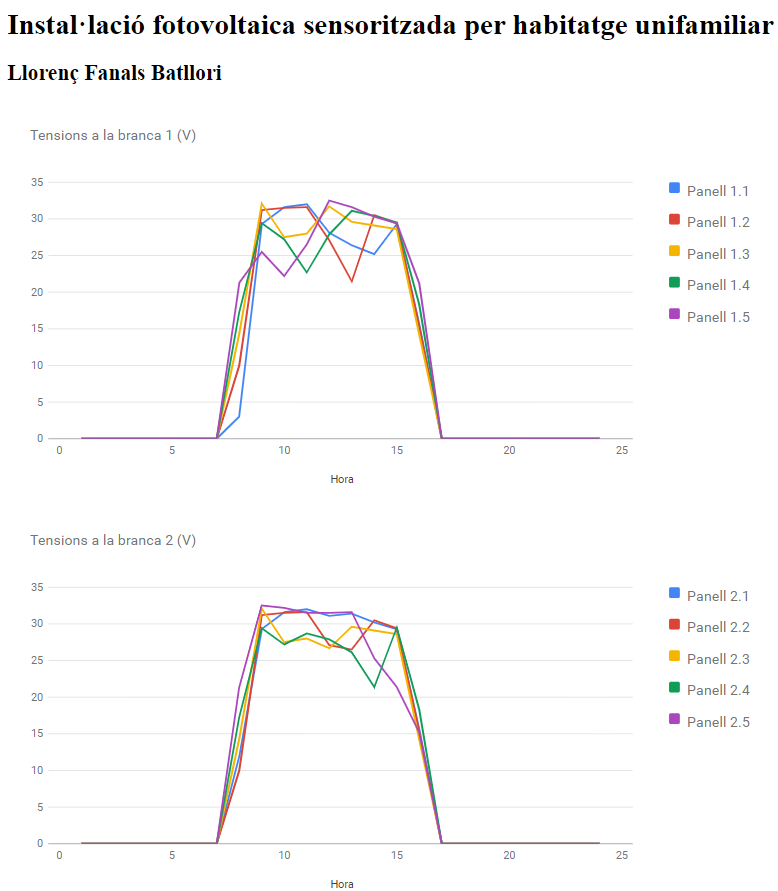
\includegraphics[scale=0.75]{images/c1.png}}
\end{center}
\caption{Part de la pàgina web}
\label{fig:1}
\end{figure}

\noindent \\ El fet d'utilitzar JavaScript permet inserir contingut dinàmic. Al passar el ratolí per sobre una línia es ressalta la línia i els punts que la formen. A la Figura \ref{fig:2} s'aprecia.
\begin{figure}[H]
\begin{center}
\fbox{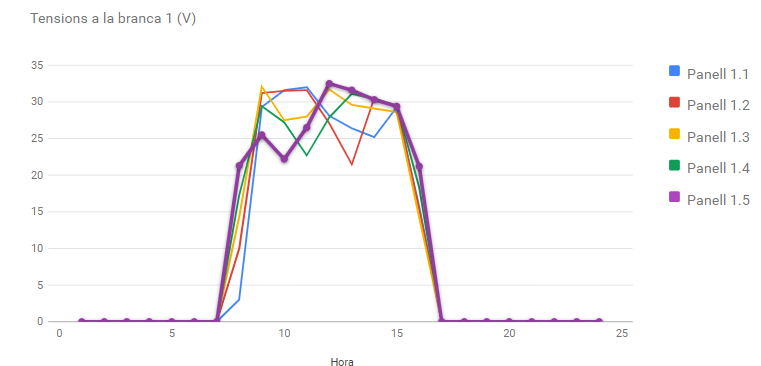
\includegraphics[scale=0.75]{images/c2.png}}
\end{center}
\caption{Gràfica d'un panell i punts ressaltats}
\label{fig:2}
\end{figure}

\noindent A més, és possible visualitzar el valor de cada punt col·locant el ratolí sobre seu, es veu a la Figura \ref{fig:3}.
\begin{figure}[H]
\begin{center}
\fbox{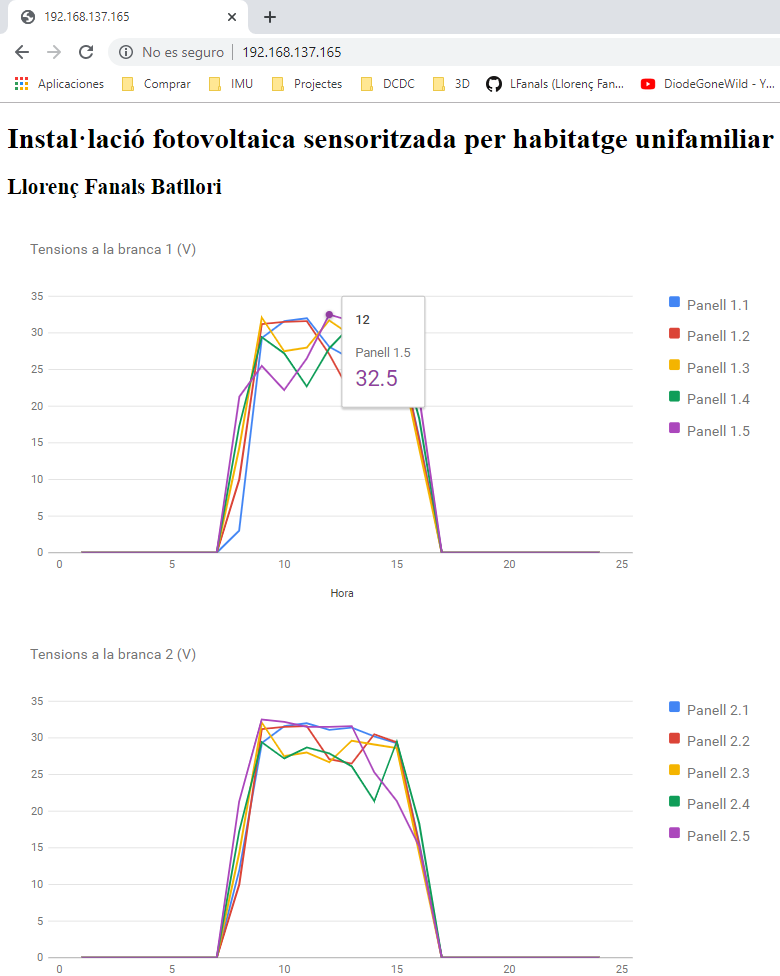
\includegraphics[scale=0.75]{images/c3.png}}
\end{center}
\caption{Gràfica d'un panell, lectura d'un dels seus punts}
\label{fig:3}
\end{figure}

\noindent A la pàgina web també s'ha inserit un croquis de la disposició de les plaques. Amb la imatge i les gràfiques el client pot deduir fàcilment quins panells estan més ombrejats, en quines hores i, en cas de tensions massa baixes, quins poden estar malmesos i necessiten ser revisats. Es mostra a la Figura \ref{fig:4}.

\begin{figure}[H]
\begin{center}
\fbox{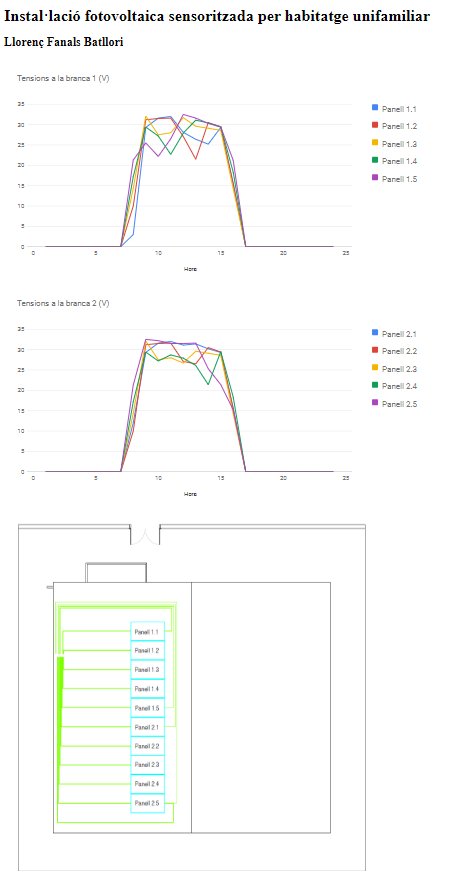
\includegraphics[scale=1.0]{images/c4.png}}
\end{center}
\caption{Pàgina web completa}
\label{fig:4}
\end{figure}





\clearpage


% Table generated by Excel2LaTeX from sheet 'Hoja1'
%\begin{table}[H]
%  \centering
%    \begin{tabularx} {\textwidth} {|X|r|} \hline
%  \multicolumn{1}{|c|}{Descripció} &  \multicolumn{1}{c|}{Quantitat}\\ \hline \hline
%
 %   Placa GLC 330 W & 10 \\ \hline
%    Inversor FRONIUS Primo 3.0-1 Light 3kW & 1 \\ \hline
%    Metres cable Ethernet RJ-45 CAT 8 & 10 \\ \hline
%    Metres cable 4 m$m^2$ PVC & 45 \\ \hline
 %   Metres cable 1,5 m$m^2$ PVC & 100 \\ \hline
 %   Punteres Enghofer E 4-10, 4 m$m^2$, 10 mm & 20 \\ \hline
 %   Punteres Enghofer E 1.5-10 1,5 m$m^2$ 10 mm & 12 \\ \hline
 %   Cinta aïllant 10 m 1,6 cm & 3 \\ \hline
 %   Caixa estanca Solera CONS 100x100x55 mm & 2 \\ \hline
  %  Canal Euroquint 25,16 mm 1,5 metres & 20 \\ \hline
%    Curva canal VECAMCO & 10 \\ \hline
%    Paquet de 50 brides 200x2,6  mm & 2 \\ \hline
%    Regleta nylon 12 pols 16 mm & 4 \\ \hline
%    Premsaestopes M12 & 10 \\ \hline
%    Cargol autoroscant M4 16 mm & 12 \\ \hline
%    Tacs Fischer 072095 nylon 6x50 mm & 50 \\ \hline
%    Díode SM74611KTTR & 10 \\ \hline
%            Hores enginyer & 1 \\ \hline
%    Hores oficial de primera & 12 \\ \hline
%    Hores oficial de segona & 12 \\ \hline
%    \end{tabularx}%
%  \label{tab:addlabel}%
% \end{table}%

%\chapter{\uppercase{Instal·lació de l'electrònica}}
% Connexionat de les plaques electròniques amb la instal·lació elèctrica.



\clearpage


% Table generated by Excel2LaTeX from sheet 'Hoja1'
%\begin{table}[H]
%  \centering
%    \begin{tabularx} {\textwidth} {|X|r|} \hline
%  \multicolumn{1}{|c|}{Descripció} &  \multicolumn{1}{c|}{Quantitat}\\ \hline \hline
%
 %   Placa GLC 330 W & 10 \\ \hline
%    Inversor FRONIUS Primo 3.0-1 Light 3kW & 1 \\ \hline
%    Metres cable Ethernet RJ-45 CAT 8 & 10 \\ \hline
%    Metres cable 4 m$m^2$ PVC & 45 \\ \hline
 %   Metres cable 1,5 m$m^2$ PVC & 100 \\ \hline
 %   Punteres Enghofer E 4-10, 4 m$m^2$, 10 mm & 20 \\ \hline
 %   Punteres Enghofer E 1.5-10 1,5 m$m^2$ 10 mm & 12 \\ \hline
 %   Cinta aïllant 10 m 1,6 cm & 3 \\ \hline
 %   Caixa estanca Solera CONS 100x100x55 mm & 2 \\ \hline
  %  Canal Euroquint 25,16 mm 1,5 metres & 20 \\ \hline
%    Curva canal VECAMCO & 10 \\ \hline
%    Paquet de 50 brides 200x2,6  mm & 2 \\ \hline
%    Regleta nylon 12 pols 16 mm & 4 \\ \hline
%    Premsaestopes M12 & 10 \\ \hline
%    Cargol autoroscant M4 16 mm & 12 \\ \hline
%    Tacs Fischer 072095 nylon 6x50 mm & 50 \\ \hline
%    Díode SM74611KTTR & 10 \\ \hline
%            Hores enginyer & 1 \\ \hline
%    Hores oficial de primera & 12 \\ \hline
%    Hores oficial de segona & 12 \\ \hline
%    \end{tabularx}%
%  \label{tab:addlabel}%
% \end{table}%


\chapter{\uppercase{Resum del pressupost}}
El pressupost inclou el pagament de la instal·lació dels panells, tota la instal·lació elèctrica, el muntatge de la placa i la programació. El pressupost és d'un total de set mil cinc-cents vint-i-dos euros amb setanta-un cèntims d'euro, sense IVA.


\clearpage
\chapter{\uppercase{Conclusió}}
Per desenvolupar el projecte s'ha consultat l'IDAE de novembre de 2019 per tal de determinar les pèrdues generades per les ombres, els angles d'orientació i inclinació, la connexió dels panells entre sí i les seves proteccions. El REBT ha servit per dimensionar correctament els cables conductors segons caigudes de tensió i criteri tèrmic. També ha estat d'utilitat per dimensionar les proteccions.\\
\newline Amb aquest projecte es detalla la instal·lació elèctrica fotovoltaica d'una casa unifamiliar connectada a la xarxa amb modalitat d'autoconsum amb compensació d'excedents. S'ha decidit la potència dels panells, passant pel dimensionament de la instal·lació i de l'inversor. Al cap de l'any, l'energia generada per les plaques fotovoltaiques és propera a la consumida.\\
\newline Per la banda de l'electrònica s'ha dissenyat el hardware que es fa servir i com les diferents parts del circuit s'adapten entre elles per donar lloc a una placa electrònica capaç de llegir les tensions de cada placa de forma correcta i publicar-les en una web.\\
\newline El client podrà visualitzar els perfils de tensió de les últimes 24 hores de cada placa. Així sabrà com han afectat les ombres i podrà detectar un possible malmetement d'algun panell. Es preveu que la realització d'aquest projecte ha de permetre al client generar energia elèctrica de forma més sostenible amb el medi ambient. \\

\vspace*{\fill}
\noindent Llorenç Fanals Batllori\\
Graduat en Enginyeria Electrònica Industrial i Automàtica\\
\\
\\
Girona, 28 de novembre de 2019.

\clearpage
\chapter{\uppercase{Relació de documents}}
El projecte està format per cinc documents, que són Memòria, Plànols, Plec de condicions, Estat d'amidaments i Pressupost.

\clearpage
\chapter{\uppercase{Bibliografia}}
CASTEJÓN, A., SANTAMARÍA, G. Instalaciones solares fotovoltaicas. Editorial Editex. 2010. \\ \\
GCL. GCL-P6/72-330 Specifications. (https://www.solaris-shop.com/content/GCL-P6-72\%20Specifications.pdf, 29 d'octubre de 2019) \\ \\
GOOGLE. Line Chart by Google Charts. (https://developers.google.com/chart/interactive/docs/
gallery/linechart?hl=es, 20 de novembre de 2019) \\ \\
KALOGIROU, S. McEvoy's Handbook of Photovoltaics. Academic Press. 2017. \\ \\
RANDOM NERD TUTORIALS. Build an ESP8266 Web Server - Code and Schematics. (https://randomnerdtutorials.com/esp8266-web-server/, 27 d'octubre de 2019) \\ \\
SOLARIS. GCL-P6/72-330 330W POLY SOLAR PANEL. (https://www.solaris-shop.com/gcl-gcl-p6-72-330-330w-poly-solar-panel/, 17 de novembre de 2019) \\ \\
TEXAS INSTRUMENTS. High-Speed CMOS Logic, 16-Channel Analog Multiplexer/Demultiplexer. (https://www.ti.com/lit/ds/symlink/cd74hc4067.pdf, 20 de novembre 2019) \\ \\
VOWSTAR. NodeMCU Development Kit. (https://github.com/nodemcu/nodemcu-devkit-v1.0/blob/master/NODEMCU\_DEVKIT\_V1.0.PDF, 23 d'octubre de 2019)



%\clearpage
\chapter{\uppercase{Glossari}}
% ordenar alfebèticament
AC: Corrent Altern. \\ \\
API: Application Programming Interface. \\ \\
DC: Corrent Continu. \\ \\
HTML: HyperText Markyp Language. \\ \\
MPPT: Maximum Power Point Tracking. \\ \\
PV: Photovoltaic. \\ \\
QGPC: Quadre General de Protecció i Comandament. \\ \\
REBT: Reglament Electrotècnic de Baixa Tensió. \\ \\
RF: Radiofreqüència. \\ \\
RTU: Remote Terminal Unit. \\ \\
SMD: Sourface Mount Device. \\ \\
SSID: Service Set Identifier. \\ \\
USB: Universal Serial Bus. \\ \\



% PVC, AC, DC, USB, QGPC, REBT, 

\clearpage


\appendix

\chapter{\uppercase{Càlculs}}
%\section{Càlculs línies elèctriques}
Per tal de calcular les seccions mínimes de les línies es té en compte la caiguda de tensió i la intensitat màxima admissible dels cables. El REBT indica a la ITC-BT-40 que els cables de connexió hauran d'estar dimensionats per una intensitat no inferior al 125\% de la intensitat màxima del generador. A més, la caiguda de tensió màxima permesa entre el generador i el punt d'interconnexió amb la xarxa és de 1,5\% respecte la tensió nominal.\\
\newline Recordar que les línies de connexió entre els panells solars, amb l'inversor i a la placa electrònica es té una senyal elèctrica de tipus continu. La línia que connecta la sortida de l'inversor amb la instal·lació interior és de senyal alterna, i es considera que amb un factor de potència unitari. El fabricant indica que el factor de potència de l'inversor escollit és sempre molt proper a la unitat.\\
\newline Per calcular la intensitat de les línies monofàsiques es fa servir l'Equació \ref{eq:il}:
\begin{equation} \label{eq:il}
I_{linia} = \frac{P}{V*\cos(\phi)}
\end{equation}
V = 230 V.\\
P: potència que consumeixen els elements connectats a la línia (W).\\
$\phi$: factor de potència.\\
\newline En monofàsic cal fer servir l'Equació \ref{eq:e}:
\begin{equation}\label{eq:e}
e(\%)=\frac{P}{V}\frac{2*l}{k*S}
\end{equation}
l: longitud ja sigui de la fase o el neutre des del comptador a l'element més llunyà (m).\\
$k = 56 m/mm^{2}\si{\ohm}$.\\
S:secció del cable (m$m^2$).\\
%
\newline El dimensionament de les línies ha de permetre que les caigudes de tensió no superin els màxims indicats prèviament. Alhora, els cables han de poder admetre les intensitats calculades, per això ens guiem amb la taula de la ITC-19 del REBT. Finalment, cal comprovar que  l'interruptor magnetotèrmic té una intensitat nominal superior a la calculada per la línia i menor a l'admissible que marca la ITC-19.\\
\newline S'ha de tenir en compte el factor de correcció per radiació directa del Sol ($F_{sol}$), tal i com es comenta a la ITC-BT-06. S'escull un factor per radiació directa del Sol de 0,9.\\
\newline També s'ha de tenir en compte el factor de correcció per agrupament de cables ($F_{grup}$) de 0,89 per parelles de cables i de 0,75 per l'agrupament de cables que va a la placa electrònica, tal com marca la ITC-BT-06 que tracta sobre instal·lacions aèries.\\
\newline Finalment, el tercer factor és el factor de correcció per temperatura ($F_{temp}$), que s'escull de 0,9, que és el factor que s'ha d'agafar segons la ITC-BT-06 per temperatures de 50 $^\circ$C.\\
%
%
%
%
\newline Per totes les línies menys per la de connexionat la placa electrònica es té en compte un factor de 1,25, tal com marca la ITC-BT-19 per generadors. La caiguda de tensió no pot ser major de l'1,5\% respecte la tensió nominal.\\
\newline Es decideix instal·lar cables de recobriment de PVC sobre paret, muntatge C6.\\
%
\newline Amb aquests factors coneguts es pot calcular la intensitat de càlcul de les diferents línies, a partir de la qual es determinen les seccions.\\
\newline La intensitat de curtcircuit augmenta amb la temperatura un 0,055\% per grau centígrad. Es calcula a 70 C$^{\circ}$ la intensitat de curtcircuit en condicions de 1.000 W/$m^2$. La que facilita el fabricant és de 9,33 A a 25 C$^{\circ}$.\\
\newline Per conèixer la intensitat màxima de curtcircuit, en el cas més desfavorable, cal seguir l'Equació \ref{eq:isc}:
\begin{equation} \label{eq:isc}
I_{sc}(T=70\  C ^{\circ})= I_{sc} (1 + \alpha (T-25 \ C^{\circ}))
\end{equation}

\noindent $I_{sc}$: intensitat de curtcircuit del panell a 25 C$^{\circ}$ (A).\\
$\alpha$: factor lineal d'increment d'intensitat de curtcircuit per efecte de la temperatura (\%).\\
T: temperatura, en aquest cas 70 C$^{\circ}$.\\
\noindent El resultat és de 9,56 A.\\
%
\newline Per calcular la tensió màxima de circuit obert s'ha fet servir l'Equació \ref{eq:isc}:
\begin{equation} \label{eq:isc}
V_{oc}(T=-10\  C ^{\circ})= V_{oc} (1 + \beta (T-25 \ C^{\circ}))
\end{equation}
\noindent  $V_{oc}$: Tensió de circuit obert a 25 C$^{\circ}$ (V).\\
$\beta$: factor lineal de decrement de tensió de circuit obert per efecte de la temperatura (\%).\\
%
\newline La tensió de circuit obert a 25 C$^{\circ}$ és de 46,2 V. El factor lineal que indica el fabricant és de -0,32\%/C$^{\circ}$, que dona un total de 51,37 V. S'han tingut en compte pel dimensionament de la placa electrònica.\\
\newline Dit això, per calcular les seccions dels cables cal destacar que el producte de la intensitat de curtcircuit calculada per la temperatura més desfavorable multiplicada per 1,25 ha de ser igual a la secció del REBT multiplicada pels factors de radiació solar, agrupament i temperatura.\\
\newline Si s'aïlla, es pot dir que la intensitat de curtcircuit calculada multiplicada per 1,25 i dividida pels factors mencionats ha de ser admesa per les seccions dels cables del REBT.\\
\newline A la Taula \ref{tab:taulax} es detalla la intensitat de cada línia i els factors que cal tenir en compte.

\begin{table}[H]
\scriptsize
  \centering
    \begin{tabu} to \textwidth  {|X[0.3, l]|X[2, l]|X[0.5, r]|X[0.6, r]|X[0.5, r]|X[0.5, r]|X[0.5, r]|} \hline
Línia &  Descripció & Intensitat (A) & Factor generador & Factor radiació solar & Factor agrupament  & Factor temperatura\\ \hline \hline
L1 & Connexionat entre els panells solars & 9,56 & 1,25 & 0,9 & 0,89 & 0,9 \\ \hline
L2 & Connexionat de la branca 1 a l'inversor & 9,56 & 1,25 & 0,9 & 0,89 & 0,9\\ \hline
L3 & Connexionat de la branca 2 a l'inversor & 9,56 & 1,25 & 0,9 & 0,89 & 0,9\\ \hline
L4 & Connexionat de l'inversor al QGPC & 14,3 & 1,25 & 1,0 & 1,00 & 1,0 \\ \hline \hline
L5 & Línies de connexionat dels panells fotovoltaics a la placa electrònica & 0,0023 & 1,00 & 0,9 & 0,75 & 0,9 \\ \hline
	
    \end{tabu}%
  \caption{Intensitat de càlcul pel dimensionament de les línies}
    \label{tab:taulax}%
 \end{table}%

\noindent Amb aquesta intensitat de càlcul podem dimensionar les línies. Es calculen les seccions per tal d'evitar tenir un percentatge de caiguda de tensió entre els generadors i el punt de connexió a la xarxa superior de 1,5\%, tal com marca la ITC-BT-40 de generadors.\\
\newline A la Taula \ref{tab:t2} es mostren dades de les diverses línies detallades.\\
\newline L'inversor sempre intenta donar els 230 V a la seva sortida, sempre que el valor de l'entrada superi els 80 V mínims que marca el fabricant. S'ha acumulat la caiguda de tensió de la línia 1 amb la línia 2 i la 3; i la més desfavorable entre la 2 i la 3 amb la 4. La ITC-BT-19 verifica que per intensitats admissibles les seccions són correctes.
%
\begin{table}[H]
\scriptsize
\begin{center}
 \begin{tabu} to 0.985\textwidth {|X[0.5, l]|X[1.5, l]|X[0.8, r]|X[0.6, r]|X[r]|X[r]|X[r]|X[r]|X[r]|X[r]|X[0.5,r]|}%{X | c c c} 
 \hline
 Línia& Descripció & Potència (W) & cos($\phi$) & Intensitat nominal (A) & Distància màxima (m) & Seccions ($mm^{2}$) & Diàmetre tub (mm) & Caiguda de tensió (\%) & Caiguda de tensió acum. (\%)\\
 \hline \hline 

L1 & Connexionat entre els panells solars & 1.650 & 1 & 9,56 & 10 & 2x4 & 20 & 0,42 & 0,42 \\ \hline
L2 & Connexionat de la branca 1 a l'inversor & 1.650  & 1 & 9,56  & 30 & 2x10 & 20 & 0,50 & 0,92 \\ \hline 
L3 & Connexionat de la branca 2 a l'inversor & 1.650  & 1 & 9,56  & 19 & 2x6 & 25 & 0,53 & 0,95 \\ \hline 
L4 & Connexionat de l'inversor al QGPC & 3.300  & 1 & 14,35 & 6 & 2x4 + 4 & 25 & 0,38 & 1,33 \\ \hline \hline
L5 & Línies de connexionat dels panells fotovoltaics a la placa electrònica & 0,529 & 1 & 0,0038& 21 & 2x1,5 & 32 & 0,000575 & 0,000575 \\ \hline 


 \end{tabu}
 \caption{Línies detallades}
 \label{tab:t2}%
\end{center}
\end{table}

 
 
%
%




%\section{Càlculs placa electrònica}
% o hauria de dir instrumentació?



\clearpage


% Table generated by Excel2LaTeX from sheet 'Hoja1'
%\begin{table}[H]
%  \centering
%    \begin{tabularx} {\textwidth} {|X|r|} \hline
%  \multicolumn{1}{|c|}{Descripció} &  \multicolumn{1}{c|}{Quantitat}\\ \hline \hline
%
 %   Placa GLC 330 W & 10 \\ \hline
%    Inversor FRONIUS Primo 3.0-1 Light 3kW & 1 \\ \hline
%    Metres cable Ethernet RJ-45 CAT 8 & 10 \\ \hline
%    Metres cable 4 m$m^2$ PVC & 45 \\ \hline
 %   Metres cable 1,5 m$m^2$ PVC & 100 \\ \hline
 %   Punteres Enghofer E 4-10, 4 m$m^2$, 10 mm & 20 \\ \hline
 %   Punteres Enghofer E 1.5-10 1,5 m$m^2$ 10 mm & 12 \\ \hline
 %   Cinta aïllant 10 m 1,6 cm & 3 \\ \hline
 %   Caixa estanca Solera CONS 100x100x55 mm & 2 \\ \hline
  %  Canal Euroquint 25,16 mm 1,5 metres & 20 \\ \hline
%    Curva canal VECAMCO & 10 \\ \hline
%    Paquet de 50 brides 200x2,6  mm & 2 \\ \hline
%    Regleta nylon 12 pols 16 mm & 4 \\ \hline
%    Premsaestopes M12 & 10 \\ \hline
%    Cargol autoroscant M4 16 mm & 12 \\ \hline
%    Tacs Fischer 072095 nylon 6x50 mm & 50 \\ \hline
%    Díode SM74611KTTR & 10 \\ \hline
%            Hores enginyer & 1 \\ \hline
%    Hores oficial de primera & 12 \\ \hline
%    Hores oficial de segona & 12 \\ \hline
%    \end{tabularx}%
%  \label{tab:addlabel}%
% \end{table}%


\end{spacing}
\begin{spacing}{1}

\chapter{\uppercase{Programa}}
\begin{lstlisting}[style=myArduino]
/*********
Llorenç Fanals Batllori
Graduat en Enginyeria Electrònica Industrial i Automàtica
20/11/2019
*********/

#include <ESP8266WiFi.h> // Es carrega la llibreria Wi-Fi

// Credencials de la xarxa Wi-Fi a què ens volem connectar
const char* ssid     = "DESKTOP-E5M4HBA 4049";
const char* password = "E^1w1736";

// Port que volem utilitzar. El 80 és el port per defecte, així que teclejant la IP a un navegador en farem prou. Si fos un altre port la IP acabaria en ":número_port".
WiFiServer server(80);


unsigned long TempsActual = millis(); // Current time
unsigned long TempsAnterior = 0; // Previous time
const long TempsConnectat = 20000; // Define timeout time in milliseconds (example: 2000ms = 2s)


#define files 24
#define columnes 5

float vector[files][columnes]; // vector de dades
float vector2[files][columnes]; // vector de dades
int i = 0; // iterador per files
int j = 0; // iterador per columnes

#define D0 16
#define D1 5
#define D2 4
#define D3 12 // 0

#define ENTRADA_ANALOGICA A0

unsigned int hores_posada_marxa = 10; // l'hora en què es fa la posada en marxa
unsigned int minuts_posada_marxa = 23; // a les 10:23 es fa la posada en marxa

unsigned int hora_actual;
unsigned int minuts_actual;
unsigned int millis_anteriors;

void inicialitza_vectors(){ // Emplena els vectors de dades fictícies. A còpia d'hores s'aniran reemplaçant per dades reals
  
  vector[0][0]=0; vector[0][1]=0; vector[0][2]=0; vector[0][3]=0; vector[0][4]=0;
  vector[1][0]=0; vector[1][1]=0; vector[1][2]=0; vector[1][3]=0; vector[1][4]=0;
  vector[2][0]=0; vector[2][1]=0; vector[2][2]=0; vector[2][3]=0; vector[2][4]=0;
  vector[3][0]=0; vector[3][1]=0; vector[3][2]=0; vector[3][3]=0; vector[3][4]=0;
  vector[4][0]=0; vector[4][1]=0; vector[4][2]=0; vector[4][3]=0; vector[4][4]=0;
  vector[5][0]=0; vector[5][1]=0; vector[5][2]=0; vector[5][3]=0; vector[5][4]=0;
  vector[6][0]=0; vector[6][1]=0; vector[6][2]=0; vector[6][3]=0; vector[6][4]=0;
  vector[7][0]=3; vector[7][1]=10; vector[7][2]=14.3; vector[7][3]=17.2; vector[7][4]=21.3;
  vector[8][0]=29.3; vector[8][1]=31.2; vector[8][2]=32.1; vector[8][3]=29.4; vector[8][4]=25.5;
  vector[9][0]=31.6; vector[9][1]=31.5; vector[9][2]=27.5; vector[9][3]=27.2; vector[9][4]=22.2;
  vector[10][0]=32.0; vector[10][1]=31.6; vector[10][2]=28; vector[10][3]=22.7; vector[10][4]=26.5;
  vector[11][0]=28.1; vector[11][1]=27.1; vector[11][2]=31.7; vector[11][3]=27.9; vector[11][4]=32.5; // central, pic
  vector[12][0]=26.4; vector[12][1]=21.5; vector[12][2]=29.6; vector[12][3]=31.1; vector[12][4]=31.6;
  vector[13][0]=25.2; vector[13][1]=30.5; vector[13][2]=29.1; vector[13][3]=30.4; vector[13][4]=30.3;
  vector[14][0]=29.3; vector[14][1]=29.4; vector[14][2]=28.6; vector[14][3]=29.5; vector[14][4]=29.4;
  vector[15][0]=15.6; vector[15][1]=15.3; vector[15][2]=14.2; vector[15][3]=18.3; vector[15][4]=21.2;
  vector[16][0]=0; vector[16][1]=0; vector[16][2]=0; vector[16][3]=0; vector[16][4]=0;
  vector[17][0]=0; vector[17][1]=0; vector[17][2]=0; vector[17][3]=0; vector[17][4]=0;
  vector[18][0]=0; vector[18][1]=0; vector[18][2]=0; vector[18][3]=0; vector[18][4]=0;
  vector[19][0]=0; vector[19][1]=0; vector[19][2]=0; vector[19][3]=0; vector[19][4]=0;
  vector[20][0]=0; vector[20][1]=0; vector[20][2]=0; vector[20][3]=0; vector[20][4]=0;
  vector[21][0]=0; vector[21][1]=0; vector[21][2]=0; vector[21][3]=0; vector[21][4]=0;
  vector[22][0]=0; vector[22][1]=0; vector[22][2]=0; vector[22][3]=0; vector[22][4]=0;
  vector[23][0]=0; vector[23][1]=0; vector[23][2]=0; vector[23][3]=0; vector[23][4]=0;

  vector2[0][0]=0; vector2[0][1]=0; vector2[0][2]=0; vector2[0][3]=0; vector2[0][4]=0;
  vector2[1][0]=0; vector2[1][1]=0; vector2[1][2]=0; vector2[1][3]=0; vector2[1][4]=0;
  vector2[2][0]=0; vector2[2][1]=0; vector2[2][2]=0; vector2[2][3]=0; vector2[2][4]=0;
  vector2[3][0]=0; vector2[3][1]=0; vector2[3][2]=0; vector2[3][3]=0; vector2[3][4]=0;
  vector2[4][0]=0; vector2[4][1]=0; vector2[4][2]=0; vector2[4][3]=0; vector2[4][4]=0;
  vector2[5][0]=0; vector2[5][1]=0; vector2[5][2]=0; vector2[5][3]=0; vector2[5][4]=0;
  vector2[6][0]=0; vector2[6][1]=0; vector2[6][2]=0; vector2[6][3]=0; vector2[6][4]=0;
  vector2[7][0]=12; vector2[7][1]=10; vector2[7][2]=14.3; vector2[7][3]=17.2; vector2[7][4]=21.3;
  vector2[8][0]=29.3; vector2[8][1]=31.2; vector2[8][2]=32.1; vector2[8][3]=29.4; vector2[8][4]=32.5;
  vector2[9][0]=31.6; vector2[9][1]=31.5; vector2[9][2]=27.5; vector2[9][3]=27.2; vector2[9][4]=32.2;
  vector2[10][0]=32.0; vector2[10][1]=31.6; vector2[10][2]=28; vector2[10][3]=28.7; vector2[10][4]=31.5;
  vector2[11][0]=31.1; vector2[11][1]=27.1; vector2[11][2]=26.7; vector2[11][3]=27.9; vector2[11][4]=31.5; // central, pic
  vector2[12][0]=31.4; vector2[12][1]=26.5; vector2[12][2]=29.6; vector2[12][3]=26.1; vector2[12][4]=31.6;
  vector2[13][0]=30.2; vector2[13][1]=30.5; vector2[13][2]=29.1; vector2[13][3]=21.4; vector2[13][4]=25.3;
  vector2[14][0]=29.3; vector2[14][1]=29.4; vector2[14][2]=28.6; vector2[14][3]=29.5; vector2[14][4]=21.4;
  vector2[15][0]=15.6; vector2[15][1]=15.3; vector2[15][2]=14.2; vector2[15][3]=18.3; vector2[15][4]=15.2;
  vector2[16][0]=0; vector2[16][1]=0; vector2[16][2]=0; vector2[16][3]=0; vector2[16][4]=0;
  vector2[17][0]=0; vector2[17][1]=0; vector2[17][2]=0; vector2[17][3]=0; vector2[17][4]=0;
  vector2[18][0]=0; vector2[18][1]=0; vector2[18][2]=0; vector2[18][3]=0; vector2[18][4]=0;
  vector2[19][0]=0; vector2[19][1]=0; vector2[19][2]=0; vector2[19][3]=0; vector2[19][4]=0;
  vector2[20][0]=0; vector2[20][1]=0; vector2[20][2]=0; vector2[20][3]=0; vector2[20][4]=0;
  vector2[21][0]=0; vector2[21][1]=0; vector2[21][2]=0; vector2[21][3]=0; vector2[21][4]=0;
  vector2[22][0]=0; vector2[22][1]=0; vector2[22][2]=0; vector2[22][3]=0; vector2[22][4]=0;
  vector2[23][0]=0; vector2[23][1]=0; vector2[23][2]=0; vector2[23][3]=0; vector2[23][4]=0;
}


void setup() {
  hora_actual = hores_posada_marxa;
  minuts_actual = minuts_posada_marxa;

  // Configurem els pins digital com a sortides per actuar sobre el multiplexor
  pinMode(D0, OUTPUT);
  pinMode(D1, OUTPUT);
  pinMode(D2, OUTPUT);
  pinMode(D3, OUTPUT);

  // Dades temporals dels vectors. Serveixen per mostrar com queden representades les gràfiques. S'aniran borrant les dades més antigues.
  inicialitza_vectors();
  
  Serial.begin(115200); // Habilitem el port sèrie a 115200 de baud rate 

  // Ens connectem al Wi-Fi amb l'adreça i la contrasenya definits
  Serial.print("Connectant a: ");
  Serial.println(ssid); // Mostrem l'adreça del Wi-Fi
  WiFi.begin(ssid, password); // Iniciem la comunicació
  
  while (WiFi.status() != WL_CONNECTED) {
    delay(500);
    Serial.print("."); // Cada 0,5 s que passin sense connectar-se mostra un punt
  }
  
  // S'ha connectat
  Serial.println("");
  Serial.println("WiFi connectat");
  Serial.println("Adreça IP: ");
  Serial.println(WiFi.localIP());
  server.begin();
  
}


void loop(){
  WiFiClient client = server.available();   // Escolta si hi ha clients

  if (client) {                             // Si es connecta un nou client,
    Serial.println("Nou client.");          
    String LiniaActual = "";                // una cadena memoritza la informació enviada pel client
    TempsActual = millis();
    TempsAnterior = TempsActual;
    while (client.connected() && TempsActual - TempsAnterior <= TempsConnectat) { // Si estem connectats i no han passat els milisegons que indica TempsConnectat,
      TempsActual = millis();         
      if (client.available()) {             // Si el client ens passa informació,
        char c = client.read();             // llegim un caràcters ascii (un byte)
        Serial.write(c);                    // i el mostrem per pantalla
        if (c == '\n') {                    // Si rebem un canvi de línia com a caràcter,
          // és el final de la petició HTTP
          if (LiniaActual.length() == 0) {
            // Ara responem donant un OK i indicant el content type, volem una pàgina html. Finalment una línia en blanc, és el protocol
            client.println("HTTP/1.1 200 OK");
            client.println("Content-type:text/html");
            client.println("Tancant connexió");
            client.println();
      
            // Al navegador volem veure una web normal i corrent que es programa amb etiquetes HTML, alguna classe CSS i serveis JavaScript
            
            client.println("<!DOCTYPE html><html>");
            client.println("<head><meta name=\"viewport\" content=\"width=device-width, initial-scale=1\">");
            client.println("<link rel=\"icon\" href=\"data:,\">");

            // Definim la gràfica de la primera branca
            client.println("<script type=\"text/javascript\" src=\"https://www.gstatic.com/charts/loader.js\"></script>\n    <script type=\"text/javascript\">\n      google.charts.load('current', {'packages':['line']});\n      google.charts.setOnLoadCallback(drawChart);\n\n    function drawChart() {\n\n      var data = new google.visualization.DataTable();\n      data.addColumn('number', 'Hora');\n      data.addColumn('number', 'Panell 1.1');\n      data.addColumn('number', 'Panell 1.2');\n      data.addColumn('number', 'Panell 1.3');\n      data.addColumn('number', 'Panell 1.4');\n      data.addColumn('number', 'Panell 1.5');\n\n");
            client.println("data.addRows([\n");
            for (i=0; i<files; i++){
                client.println("[");
                client.println(String(i+1)); 
                client.println(",");
                client.println(String(vector[i][0]));
                for (j=1; j<columnes; j++){
                  client.println(","); client.println(String(vector[i][j]));
                }  
                client.println("]"); client.println(","); client.println("\n");
            }
            client.println("]);\n\n\n      var options = {\n        chart: {\n          title: 'Tensions a la branca 1 (V)',\n          // subtitle: 'in millions of dollars (USD)'\n        },\n     //   width: 900,\n     //   height: 500\n      };\n\n      var chart = new google.charts.Line(document.getElementById('linechart_material'
            ));\n\n      chart.draw(data, google.charts.Line.convertOptions(options));\n    }\n    </script>\n");

            // Definim la gràfica de la segona branca
            client.println("    <script type=\"text/javascript\" src=\"https://www.gstatic.com/charts/loader.js\"></script>\n    <script type=\"text/javascript\">\n    google.charts.load('current', {'packages':['line']});\n    google.charts.setOnLoadCallback(drawChart);\n    \n\n    function drawChart() {\n\n    var data = new google.visualization.DataTable();\n    data.addColumn('number', 'Hora');\n    data.addColumn('number', 'Panell 2.1');\n      data.addColumn('number', 'Panell 2.2');\n      data.addColumn('number', 'Panell 2.3');\n      data.addColumn('number', 'Panell 2.4');\n      data.addColumn('number', 'Panell 2.5');\n\n");
            client.println("data.addRows([\n");
            for (i=0; i<files; i++){
                client.println("[");
                client.println(String(i+1)); 
                client.println(",");
                client.println(String(vector2[i][0]));
                for (j=1; j<columnes; j++){
                  client.println(","); client.println(String(vector2[i][j]));
                }  
                client.println("]"); client.println(","); client.println("\n");
            }
            client.println(" ]); \n\n\n\n    var options = {\n        chart: {\n        title: 'Tensions a la branca 2 (V)',\n       // is3D: true\n        // subtitle: 'in millions of dollars (USD)'\n        },\n     //   width: 700,\n     //   height: 400\n    };\n\n    var chart = new google.charts.Line(document.getElementById('linechart_material2'
            ));\n\n    chart.draw(data, google.charts.Line.convertOptions(options));\n    }\n    </script>");

           
            // Definim els títols de la pàgina, el que en HTML es coneix com a headings. Alguns caràcters en català no són ben representats, cal corregir-ho
            client.println("<body><h1 align=\"left\">Instal&middotlaci&oacute fotovoltaica sensoritzada per habitatge unifamiliar</h1>"); // &middot =  , &oacute = ó
            client.println("<h2 align=\"left\">Lloren&ccedil Fanals Batllori</h2>"); // &ccedil = ç

            client.println("<div id=\"linechart_material\" style=\"width: 800px; height: 400px; padding: 25px\"></div>  \n"); // Inserim les gràfiques del primer grup de plaques
            client.println("<div id=\"linechart_material2\" style=\"width: 800px; height: 400px; padding: 25px\"></div> "); // Inserim les gràfiques del segon grup de plaques
          
            client.println("<img src=\"https://drive.google.com/uc?export=view&id=15-EkLWMhYaR
            sv-dtbyrlKOrbD7dY71B2\"\n   align=\"left\"      style=\"width: 700px; height: 700px;  padding: 25px\" alt=\"Croquis de les plaques a la teulada\">"); // Inserim imatge del nom de cada panell
 
            client.println("</body></html>"); // Pàgina finalitzada
            
            client.println(); // Línia en blanc per finalitzar la comunicació
            
            break; // Sortim del while()
          } 
          
          else { // si tens una nova línia, neteja LiniaActual
            LiniaActual = "";
          }
          
        } 
       
        else if (c != '\r') {  // Si tens algun caràcter afegiex-lo al final de LiniaActual
          LiniaActual += c;   
        }
        
      }
    }

    // Tanquem la connexió, esperant un nou client o que el client existent refresqui la pàgina
    client.stop();
    Serial.println("Client desconnectat.");
    Serial.println("");
  }

    // Mirem si cal actualitzar els minuts i les hores i si cal fer una lectura de tensions
    comprova_temps();

  //
//  Serial.println(analogRead(ENTRADA_ANALOGICA));
//  Serial.println(millis());
}




// Encapcem amb funcions

void comprova_temps(){
    if ((millis() - millis_anteriors) >= 60000){ // ha passat un minut
        minuts_actual++;
        millis_anteriors = millis(); // memoritzem el moment en què això ha passat
        if (minuts_actual >= 60){ // si portem 60 minuts, diem que en portem 0 i incrementem l'hora
            minuts_actual = 0;
            hora_actual++;
            lectura_tensions(); // cridem la funció que llegeix les tensions
        }
        if (hora_actual >= 24){ // si l'hora és 24, la passem a 0
            hora_actual = 0;  
        }
    }
}

void lectura_tensions(){
    float tensio_superior = 0;
    float tensio_inferior = 0;
    float guany_bit_tensio = 0.0476288*3.3; // relació entre volts i bits llegits
    int memoria_ms = 0;
    int ms_delay = 20;
    
    digitalWrite(D3, LOW); digitalWrite(D2, LOW); digitalWrite(D1, LOW); digitalWrite(D0, LOW);
    memoria_ms = millis();
    while ((millis() - memoria_ms) < ms_delay){}
    vector[hora_actual][0] = analogRead(ENTRADA_ANALOGICA) * guany_bit_tensio;

    digitalWrite(D3, LOW); digitalWrite(D2, LOW); digitalWrite(D1, LOW); digitalWrite(D0, HIGH);
    memoria_ms = millis();
    while ((millis() - memoria_ms) < ms_delay){}
    vector[hora_actual][1] = analogRead(ENTRADA_ANALOGICA) * guany_bit_tensio;

    digitalWrite(D3, LOW); digitalWrite(D2, LOW); digitalWrite(D1, HIGH); digitalWrite(D0, LOW);
    memoria_ms = millis();
    while ((millis() - memoria_ms) < ms_delay){}
    vector[hora_actual][2] = analogRead(ENTRADA_ANALOGICA) * guany_bit_tensio;

    digitalWrite(D3, LOW); digitalWrite(D2, LOW); digitalWrite(D1, HIGH); digitalWrite(D0, HIGH);
    memoria_ms = millis();
    while ((millis() - memoria_ms) < ms_delay){}
    vector[hora_actual][3] = analogRead(ENTRADA_ANALOGICA) * guany_bit_tensio;

    digitalWrite(D3, LOW); digitalWrite(D2, HIGH); digitalWrite(D1, LOW); digitalWrite(D0, LOW);
    memoria_ms = millis();
    while ((millis() - memoria_ms) < ms_delay){}
    vector[hora_actual][4] = analogRead(ENTRADA_ANALOGICA) * guany_bit_tensio;

// Ara la mateixa idea però pel vector 2

    digitalWrite(D3, LOW); digitalWrite(D2, HIGH); digitalWrite(D1, LOW); digitalWrite(D0, HIGH);
    memoria_ms = millis();
    while ((millis() - memoria_ms) < ms_delay){}
    vector2[hora_actual][0] = analogRead(ENTRADA_ANALOGICA) * guany_bit_tensio;

    digitalWrite(D3, LOW); digitalWrite(D2, HIGH); digitalWrite(D1, HIGH); digitalWrite(D0, LOW);
    memoria_ms = millis();
    while ((millis() - memoria_ms) < ms_delay){}
    vector2[hora_actual][1] = analogRead(ENTRADA_ANALOGICA) * guany_bit_tensio;

    digitalWrite(D3, LOW); digitalWrite(D2, HIGH); digitalWrite(D1, HIGH); digitalWrite(D0, HIGH);
    memoria_ms = millis();
    while ((millis() - memoria_ms) < ms_delay){}
    vector2[hora_actual][2] = analogRead(ENTRADA_ANALOGICA) * guany_bit_tensio;

    digitalWrite(D3, HIGH); digitalWrite(D2, LOW); digitalWrite(D1, LOW); digitalWrite(D0, LOW);
    memoria_ms = millis();
    while ((millis() - memoria_ms) < ms_delay){}
    vector2[hora_actual][3] = analogRead(ENTRADA_ANALOGICA) * guany_bit_tensio;

    digitalWrite(D3, HIGH); digitalWrite(D2, LOW); digitalWrite(D1, LOW); digitalWrite(D0, HIGH);
    memoria_ms = millis();
    while ((millis() - memoria_ms) < ms_delay){}
    vector2[hora_actual][4] = analogRead(ENTRADA_ANALOGICA) * guany_bit_tensio;
  
}

\end{lstlisting}




\clearpage


% Table generated by Excel2LaTeX from sheet 'Hoja1'
%\begin{table}[H]
%  \centering
%    \begin{tabularx} {\textwidth} {|X|r|} \hline
%  \multicolumn{1}{|c|}{Descripció} &  \multicolumn{1}{c|}{Quantitat}\\ \hline \hline
%
 %   Placa GLC 330 W & 10 \\ \hline
%    Inversor FRONIUS Primo 3.0-1 Light 3kW & 1 \\ \hline
%    Metres cable Ethernet RJ-45 CAT 8 & 10 \\ \hline
%    Metres cable 4 m$m^2$ PVC & 45 \\ \hline
 %   Metres cable 1,5 m$m^2$ PVC & 100 \\ \hline
 %   Punteres Enghofer E 4-10, 4 m$m^2$, 10 mm & 20 \\ \hline
 %   Punteres Enghofer E 1.5-10 1,5 m$m^2$ 10 mm & 12 \\ \hline
 %   Cinta aïllant 10 m 1,6 cm & 3 \\ \hline
 %   Caixa estanca Solera CONS 100x100x55 mm & 2 \\ \hline
  %  Canal Euroquint 25,16 mm 1,5 metres & 20 \\ \hline
%    Curva canal VECAMCO & 10 \\ \hline
%    Paquet de 50 brides 200x2,6  mm & 2 \\ \hline
%    Regleta nylon 12 pols 16 mm & 4 \\ \hline
%    Premsaestopes M12 & 10 \\ \hline
%    Cargol autoroscant M4 16 mm & 12 \\ \hline
%    Tacs Fischer 072095 nylon 6x50 mm & 50 \\ \hline
%    Díode SM74611KTTR & 10 \\ \hline
%            Hores enginyer & 1 \\ \hline
%    Hores oficial de primera & 12 \\ \hline
%    Hores oficial de segona & 12 \\ \hline
%    \end{tabularx}%
%  \label{tab:addlabel}%
% \end{table}%


\begin{appendices}
%\chapter{Títol de l'annex}

%\chapter{\uppercase{Càlculs}}
Pel càlcul de les seccions dels conductors cal tenir en compte els factors de simultaneïtat d'alguns elements i els factors que marca el REBT: 1,25 pel motor elèctric de més potència de la línia, tal com es detalla a la ITC-47; i 1,8 per les lluminàries amb descàrrega, tal com s'indica a la ITC-44. A l'obrador hi ha molts motors elèctric però cap llum amb descàrrega.\\
\newline
En algunes línies es considera que el factor de potència és unitari. A la realitat mai valdrà exactament 1, però sí que es preveu que tingui un valor molt semblant. Les màquines que s'han escollit tenen un factor de potència proper a l'unitari però diferent de 1.\\
\newline Per calcular la intensitat de les línies monofàsiques es fa servir la següent fórmula:
\begin{equation}
I_{linia} = \frac{P}{V*\cos(\phi)}
\end{equation}
V = 230 V\\
P és la potència que consumeixen els elements connectats a la línia\\
$\phi$ és el factor de potència\\
\newline En trifàsic, l'equació que s'utilitza és:
\begin{equation}
I_{linia} = \frac{P}{\sqrt3*V_{linia}*\cos(\phi)}
\end{equation}
$V_{linia}$ = 400 V\\
\newline És important calcular la caiguda de tensió a les línies per tal de veure si estan dimensionades correctament. La caiguda de tensió en línies d'enllumenat no pot ser superior al 3\% i en línies de força no pot ser superior al 5\% de la tensió de subministrament. La caiguda de tensió màxima a la derivació individual és de 1,5\%.\\
\newline En monofàsic:
\begin{equation}
e(\%)=\frac{P}{V}\frac{2*l}{k*S}
\end{equation}
l és la longitud ja sigui de la fase o el neutre des del comptador a l'element més llunyà\\
$k = 56 \frac{m}{mm^{2}\si{\ohm}}$\\
S és la secció del cable en m$m^2$\\
\newline
En trifàsic, l'equació que s'utilitza és:
\begin{equation}
e(\%)=\frac{P}{V}\frac{l}{k*S}
\end{equation}
\\
El dimensionament de les línies ha de permetre que les caigudes de tensió no superin els màxims indicats prèviament. Alhora, els cables han de poder admetre les intensitats calculades, per això ens guiem amb la taula de la ITC-19 del REBT. Finalment, cal comprovar que  l'interruptor magnetotèrmic té una intensitat nominal superior a la calculada per la línia i menor a l'admissible que marca la ITC-19.\\
\newline La instal·lació és trifàsica, per tant, hi ha 3 conductors de fase i un conductor de neutre. El conductor de terra transcorre per totes les línies i té una secció igual als conductors de les línies, tal com s'indica al plànol. El neutre, que arriba per l'escomesa, també és de la mateixa secció que els conductors de fase. Les màquines trifàsiques necessiten el neutre pels seus equips electrònics.\\
\newline
Per comprovar que el valor de secció de la derivació individual és correcte quan la línia va amb una terna de cables unipolars per tub cal tenir en compte un factor d'intensitat de 0,8.
\begin{equation}
I_{DI} < 0.8 * I_{max. admissible}
\end{equation}

\noindent A continuació es mostren les diferents línies de forma detallada. La secció s'ha comprovat tenint en compte les fórmules explicades i les seccions mínimes per intensitat segons marca el REBT. S'han verificat les línies pel cas més desfavorable. Les seccions dels tubs compleixen amb la ITC-21.\\
\newline Les tensions nominals són 230 V per les línies monofàsiques i 400 V per les trifàsiques. Tots els cables de les línies són de coure de 450/750 V d'aïllament. La derivació individual és de coure amb 0,6/1 kV d'aïllament. L'aïllament de la instal·lació és de 1.000 k$\si{\ohm}$.

\begin{table}[H]
\scriptsize
\begin{center}
 \begin{tabu} to \textwidth {|X[0.5, l]|X[2, l]|X[r]|X[0.6, r]|X[r]|X[r]|X[r]|X[r]|X[r]|X[r]|X[0.5,r]|}%{X | c c c} 
 \hline
 Línia& Descripció & Potència (W) & cos($\phi$) & Intensitat (A) & Distància màxima (m) & Seccions fase, neutre, terra ($mm^{2}$) & Diàmetre tub (mm) & Caiguda de tensió (\%) & Caiguda de tensió acum. (\%)\\
 \hline \hline 
DI & Derivació individual& 87.000 \ \ \ \ & 0,96 & 131,32 & 8 &3x35 + 35 + 16& 160 & 0,23 & 0,23 \\ \hline
L1 & Enllumenat habitacions i cambra& 1.370,5 & 1 & 5,96 & 55 &2,5 + 2,5 + 2,5& 20 & 2,04 & 2,27 \\ \hline
L2 & Enllumenat cuina & 1.476 \ \ \ \  & 1 & 6,42 & 47 &2,5 + 2,5 + 2,5& 20 & 1,87 & 2,10 \\ \hline 
L3 & Força oficina, menjador, màquines de buit & 7.775 \ \ \ \  & 1 & 33,80 & 51 &10 + 10 + 10& 25 & 2,68 & 2,91 \\ \hline 
L4 & Força cuina & 7.235 \ \ \ \  & 1 & 31,46 & 33 & 6 + 6 + 6& 25 & 2,67 & 2,90 \\ \hline
L5 & Rentaplats cuina & 36.000 \ \ \ \ & 0,95 & 54,92 & 54 &3x16 + 16 + 16& 32 & 1,44 & 1,67 \\ \hline 
L6 & Extractors i cambres de fred & 19.000 \ \ \ \ & 0,9 & 30,60 & 36 &3x10 + 10 + 10& 32 & 0,86 & 1,09 \\ \hline
L7 & Abatidor sala de preparació & 16.975 \ \ \ \ & 0,95 & 25,90 & 44 &3x10 + 10 + 10& 32 & 0,84 & 1,07 \\ \hline

 \end{tabu}
 \caption{Línies detallades}
\end{center}
\end{table}



%\chapter{\uppercase{Característiques}}
L'aïllament dels cables elèctrics de les línies és EPR de 450/750 V d'aïllament. Els cables transcorren en safata perforada pel passadís i dins de tubs corrugats en muntatge superficial (B2) a la resta de zones. El diàmetre d'aquests tubs s'indica en l'anterior annex. Els càlculs s'han efectuat considerant que tota la llargada dels cables va amb el muntatge B2, que és més restrictiu que la safata.\\
\newline Es fan servir els colors gris, marró i negre per les fases, el blau pel neutre i el conductor groc i verd pel terra.\\
\newline Hi ha instal·lades caixes de derivació al llarg de la instal·lació i l'enllumenat dels vestidors, l'oficina i el menjador es controla amb interruptors de paret. Els cables dels l'enllumenats que no estan en contacte amb la paret es passen pel fals sostre.\\
\newline Les màquines trifàsiques es connecten a la xarxa mitjançant una base CETAC.\\
\newline Els extractors de la cuina de l'obrador van controlats amb variadors de freqüència. La seva línia va amb un diferencial de 100 mA de classe B degut als alts corrents de fuga que poden donar-se. Aigües amunt de tots els agrupaments hi ha instal·lat un diferencial de 300 mA de sensibilitat per protegir tota la instal·lació i alhora tenir selectivitat amb el diferencials que té aigües avall.\\
\newline El maxímetre del conjunt de protecció i mesura garanteix el subministrament elèctric tot i sobrepassar la potència contractada. Si en un moment puntual es connectés alguna màquina més i pel marge donat no saltés cap interruptor magnetotèrmic però s'estigués superant la potència contractada, hi seguiria havent subministrament elèctric i l'empresa subministradora aplicaria un recàrrec a la factura.\\
\newline 
S'agrupen les línies tenint en compte si el subministrament és trifàsic o monofàsic. S'intenta, en la mesura del possible, que tots els grups tinguin potències similars. És per això que el diferencial que agrupa les 4 línies monofàsiques és de 4 pols: els 3 conductors de fase i el neutre passaran per aquest diferencial i s'alimentaran les diferents línies monofàsiques amb diferents fases. Així es pot aconseguir una instal·lació trifàsica bastant ben equilibrada.\\
\newline Els llums d'emergència són de tipus no permanent i es considera que tenen una potència de 3 W. Al disposar de bateria i només encendre's quan hi ha una emergència, no s'han tingut en compte per la previsió de càrregues.\\
\newline Per millorar el factor de potència de la derivació individual, o sigui, de tota la instal·lació, hi ha instal·lada una bateria de condensadors de 20 kVAr la qual dona una factor de potència de 0,998.




\end{appendices}


\end{spacing}
%\cite{einstein} % per fer una cita
%\printbibliography[title=Bibliografia] %ARA BÉ

\end{document}